Die in dieser Arbeit vorgestellten Methoden wurden auf chemische Fragestellungen angewendet, um die experimentellen Befunde zu unterstützen oder besser deuten zu können.
Der erste Abschnitt dieses Kapitels widmet sich der Untersuchung von Ringströmen in großen toroidalen Kohlenstoff-Nanoröhren mit bis zu 1000 Atomen, wofür die von einem äußeren Magnetfeld hervorgerufene Störung der Elektronendichte (\textit{magnetic response}) benötigt wird. Durch die in dieser Arbeit implementierten Methoden zur Verbesserung der Effizienz wurde die Berechnung der entsprechenden Dichtematrix in einem akzeptablen Zeitrahmen auch für Systeme dieser Größe ermöglicht. Im zweiten Abschnitt dieses Kapitels wird die Anwendung der quantenchemischen Methoden auf eine Reihe anorganischer Verbindungen beschrieben.  

\section{Ringströme in großen toroidalen Kohlenstoff-Nanoröhren}
1991 beschrieb Iijima\supercite{iijima1991helical} die Herstellung eines neuen Strukturtyps des Kohlenstoffs bestehend aus aufgerollten Graphenschichten, die Kohlenstoff-Nanoröhren (englisch \acp{cnt}). Im geometrischen Sinne können ideale \acp{cnt} durch Aufrollen perfekter Graphenschichten konstruiert werden und bestehen demzufolge aus verknüpften, sechsgliedrigen Kohlenstoffringen. \acp{cnt} lassen sich in chirale und achirale Strukturen unterteilen, wobei letztere entweder dem \textit{armchair}- oder \textit{zigzag}-Typ angehören. Der Chiralitätsvektor $\vec{\text{C}}_\text{h}$ wird dabei durch die beiden Parameter $(n,m)$ beschrieben und zeigt die Richtung an, in welcher die Graphenschicht aufgerollt wird. Seine Länge definiert demnach den Umfang und $\frac{\vert\vec{\text{C}}_\text{h}\vert}{2\pi}$ den Radius der resultierenden Nanoröhre. \acp{cnt} mit einer finiten Länge lassen sich durch einen weiteren Vektor $\vec{\text{T}}$, definiert durch die beiden zusätzlichen Parameter $(p,q)$, eindeutig beschreiben. Dieser zeigt in Richtung der Röhrenachse und gibt deren Länge an. Das grundlegende Konstruktionsschema ist in Abbildung \ref{abb:chiralvector} gezeigt. Aufgerollt ergibt die darin eingezeichnete graue Fläche die chirale Kohlenstoff-Nanoröhre mit den Parametern $(n=3,m=1),(p=3,q=\textrm{-}4)$.
\begin{figure}[ht!]
	\centering
	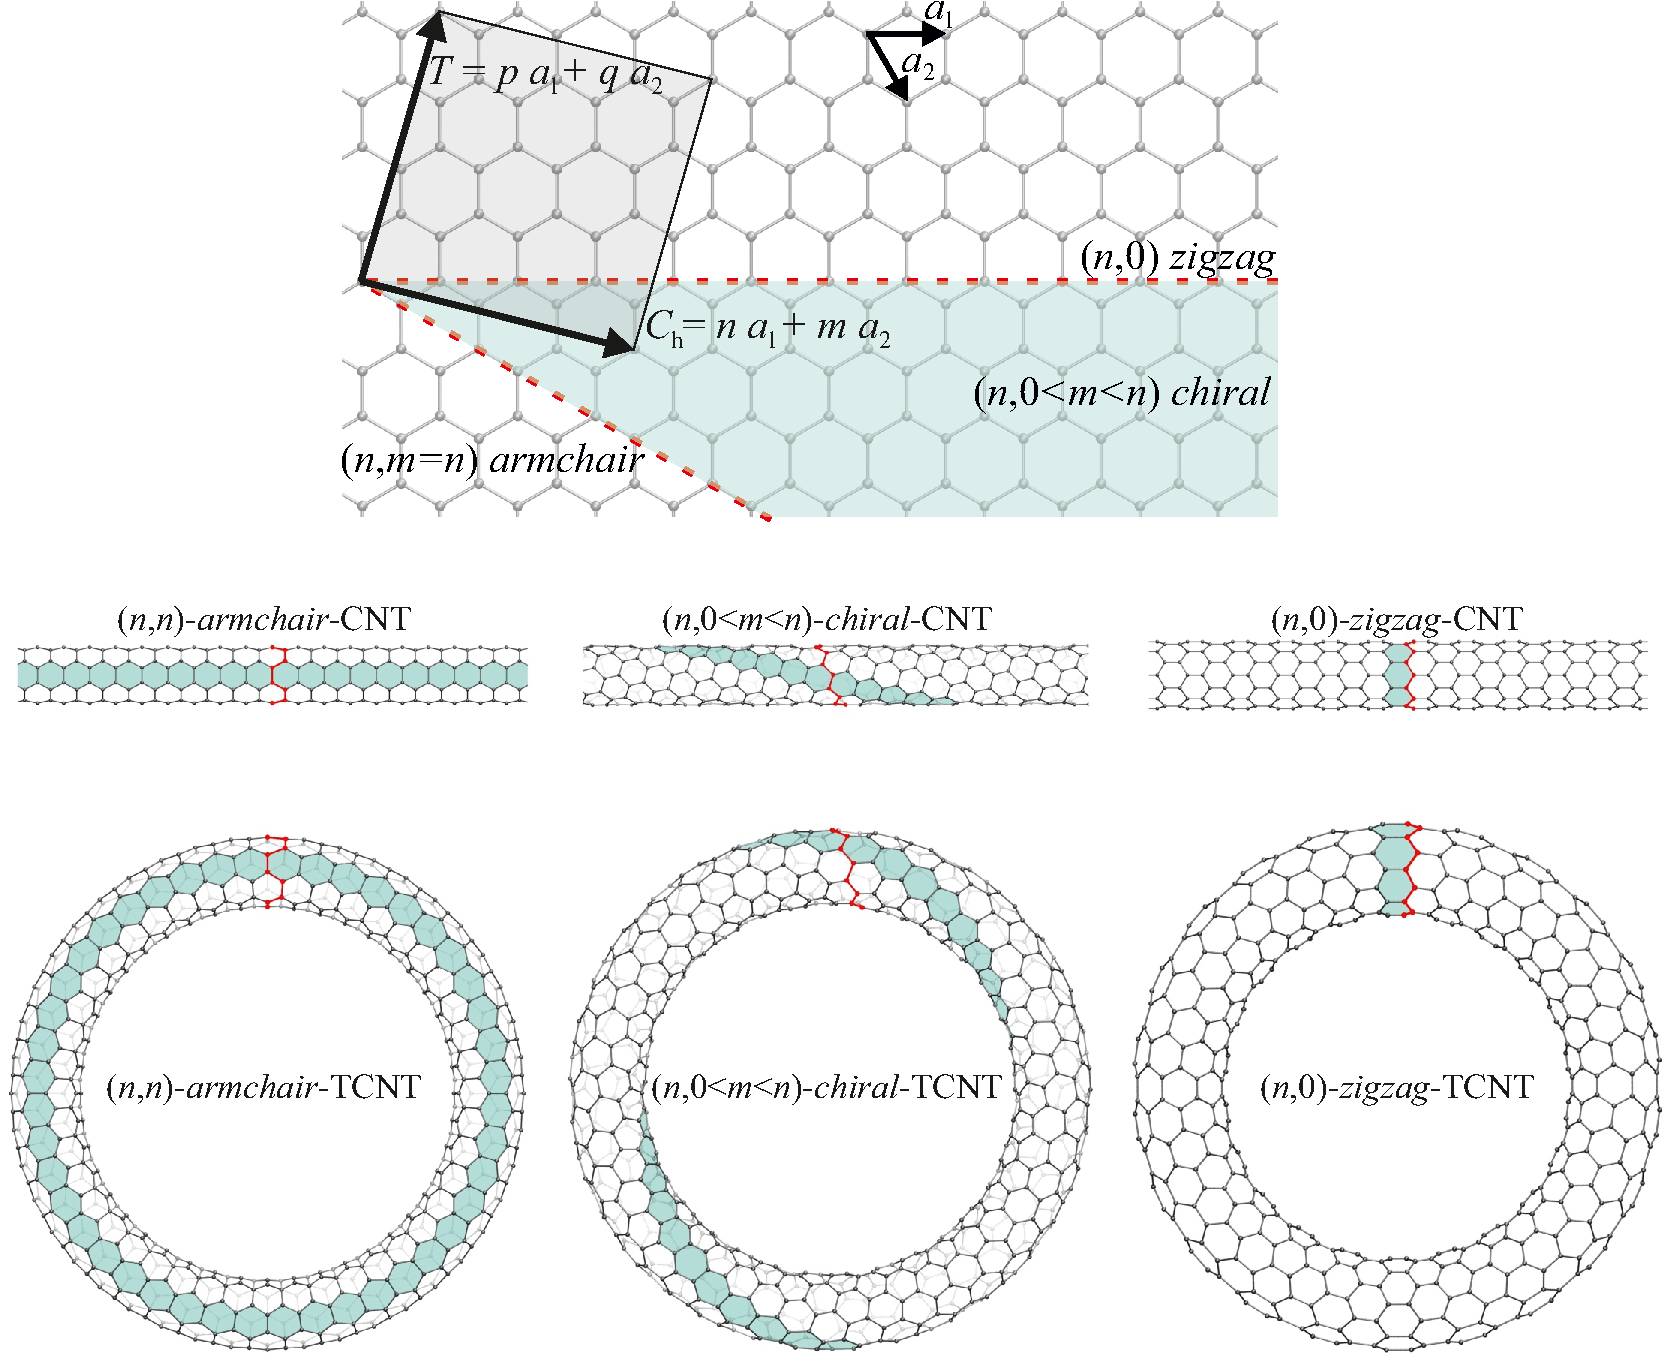
\includegraphics[width=1.0\textwidth]{vector}
	\captionsetup{figurewithin = chapter}
	\captionsetup{font=small, labelfont=bf}\caption[Allgemeines Konstruktionsschema von (toroidalen \textit{polyhex}-)Kohlenstoff-Nanoröhren]{Allgemeines Konstruktionsschema für Kohlenstoff-Nanoröhren \textsf{(a)}. $a_1$ und $a_2$ sind die Basisvektoren der Elementarzelle von Graphen. Der Chiralitätsvektor $\vec{\text{C}}_\text{h}$ liegt in dem türkis eingefärbten Bereich und die gestrichelten roten Linien geben die achiralen Grenzfälle (\textit{armchair} und \textit{zigzag}) an. Der Vektor $\vec{\text{T}}$ beschreibt die Länge von finiten Röhren und $n,m,p,q$ sind ganze Zahlen. Die grau eingefärbte Fläche definiert damit eine $(n=3,m=1),(p=3,q=\textrm{-}4)$-\ac{cnt}. Struktur von \acp{cnt} \textsf{(b)} und zu Ringen gebogene \textit{polyhex}-\acp{tcnt} \textsf{(c)} mit unterschiedlichen Chiralitätsvektoren.}
\label{abb:chiralvector}
\end{figure}
\vfill
\FloatBarrier
\newpage

Bereits kurz nach Entdeckung der geraden Kohlenstoff-Nanoröhren rückten auch gebogene Strukturen immer mehr in den Fokus der Forschung. Experimentell beobachtete \acp{cnt} beinhalten beispielsweise auch fünf- und siebengliedrige Kohlenstoffringe.\supercite{ichihashi1992pentagons} Diese Defekte führen zu positiven bzw. negativen Krümmungen, wodurch verbogene und verdrillte Strukturen entstehen. Ein besonderer Strukturtyp darunter sind die ringförmigen oder toroidalen Kohlenstoff-Nanoröhren (englisch \acfp{tcnt}), erstmals Ende der 90er-Jahre von Liu\supercite{liu1997c} beobachtet. Seitdem wurden mehrere Methoden zur Herstellung solcher \acp{tcnt} vorgestellt, beispielsweise laserinduziertes Wachstum,\supercite{liu1997c} Ultraschallbehandlungen,\supercite{martel1999rings,martel1999ring} organische Reaktionen,\supercite{sano2001ring,geng2008synthesis} thermische Zersetzung von Kohlenwasserstoffgasen\supercite{ahlskog1999ring} und \ac{cvd}\supercite{song2006large,zhou2006ring}. Diese \acp{tcnt} haben üblicherweise einen Torusdurchmesser von einigen hundert Nanometer, einen Röhrendurchmesser von etwa \unit[5--20]{nm} und können aus einwandigen \acp{cnt} (englisch \acp{swnt}),\supercite{martel1999rings,martel1999ring,sano2001ring,geng2008synthesis,komatsu2006ultrasonic,guo2007spontaneously} zweiwandigen,\supercite{colomer2003rings} dreiwandigen\supercite{yu2006rings} oder mehrwandigen\supercite{ahlskog1999ring} \acp{cnt} bestehen. Weitere Strukturtypen sind auch in einem kürzlich erschienen Übersichtsartikel\supercite{liu2014curved} zusammengefasst.

Durch ihre ringförmige Geometrie ist es denkbar, dass \acp{tcnt} andere mechanische, magnetische oder elektronische Eigenschaften als gerade \acp{cnt} aufweisen und damit potenziell in anderen Bereichen genutzt werden können.\supercite{liu2014curved} Auf theoretischer Ebene wurden bereits unterschiedliche Einsatzgebiete für \acp{tcnt} untersucht, beispielsweise zur Verwendung als Wasserstoffspeicher\supercite{castillo2010hydrogen,cruz2010hydrogen}. Aufgrund ihrer reversiblen, elastischen Eigenschaften sind \acp{tcnt} aber auch potenzielle Kandidaten für ultrasensitive Kraftsensoren und sie könnten als mechanische Federn in Nanogeräten verwendet werden.\supercite{zheng2010elastic,chen2011controlling} Ihre Eigenschaften machen einen Einsatz als elektromagnetische Hochfrequenzoszillatoren denkbar, wobei die \ac{tcnt} auf eine Nanoröhre gesteckt wird, entlang derer sie oszilliert. \supercite{hilder2007oscillating,ansari2017oscillation} Diese Systeme weisen eine extrem niedrige Reibungskraft\supercite{cumings2000low} auf und können Oszillationsfrequenzen von über 100 Gigahertz erreichen.\supercite{liu2014curved} Mögliche Anwendungsbeispiele wären die Verwendung als extrem schnelle optische Filter für faseroptische Systeme oder als Nanoantennen, welche für elektromagnetische Hochfrequenzsignale empfindlich sind.\supercite{hilder2007oscillating} Daher ist die weitere Untersuchung ihrer Eigenschaften sowohl auf experimenteller aber auch auf theoretischer Ebene von großem Interesse.

Es gibt unterschiedliche Strukturtypen von \acp{tcnt}, welche zum Teil bereits vor ihrer Herstellung auf theoretischer Ebene vorgeschlagen wurden. In diesem Abschnitt der Arbeit werden für einige Vertreter der einzelnen Strukturtypen magnetische Ringströme berechnet, um Abhängigkeiten der Stromstärken von Bauweise und Größe der Ringe ausfindig zu machen. Im Folgenden werden zunächst die verschiedenen Strukturtypen spezifiziert und im Anschluss daran die Ergebnisse vorgestellt.   
Die Strukturtypen lassen sich einteilen in perfekt toroidale Strukturen, welche nur aus sechsgliedrigen Ringen und damit aus gebogenen, perfekten \acp{cnt} bestehen (\textit{polyhex}-\acp{tcnt}), und zum anderen in Strukturen, welche fünf- und siebengliedrige Kohlenstoffringe enthalten. Die pentagonalen und heptagonalen Einheiten nehmen einen Großteil der Spannung aus dem System, wodurch deutlich kleinere Strukturen denkbar sind. Dunlab\supercite{dunlap1992connecting} schlug 1992 die Verknüpfung von $(n,n)$- und $(2n,0)$-\acp{cnt} vor, was zur Einführung von fünf- und siebengliedrigen Kohlenstoffringen und damit zur Bildung eines Torus mit sechszähliger Rotationssymmetrie führt. Zur Überprüfung einer möglichen Existenz dieser hypothetischen Strukturen wurden zahlreiche theoretische Studien über ihre thermodynamische Stabilität durchgeführt. Diese Studien zeigen, dass \acp{tcnt} beispielsweise stabiler als das C$_{60}$-Fulleren\supercite{dunlap1992connecting,itoh1993toroidal,ihara1993toroidal,itoh1993toroidal2} sein können, und \ac{md}-Simulationen\supercite{itoh1993toroidal,hod2003carbon,tacsci2005stability,chen2011thermal} sagen eine Beständigkeit der Strukturen bis ca. \unit[2000]{K} voraus. Im Bezug auf die Rotationssymmetrie der \acp{tcnt} haben sich $D_{\text{6h}}$-symmetrische Strukturen als besonders vorteilhaft herausgestellt\supercite{liu2011structure,ihara1995helically}, da die darin auftretenden Winkel den natürlichen Winkeln im Graphen am nächsten kommen und die geringste Verzerrung entsteht. Ein unteres theoretisches Limit für den Torusdurchmesser thermodynamisch stabiler \textit{polyhex}-\acp{tcnt} wurde bei etwa \unit[200]{nm} gefunden.\supercite{meunier1998atomic}\\

Je nach Ausrichtung des Chiralitätsvektors sind \acp{cnt} entweder metallisch oder nichtmetallisch, was anhand berechneter Bandstrukturen und -lücken gezeigt werden konnte.\supercite{mintmire1992fullerene,hamada1992new,saito1992electronic,saito1998physical} Diese theoretischen Vorhersagen konnten wenig später mithilfe der Rastertunnelspektroskopie auch experimentell bestätigt werden.\supercite{wilder1998electronic} Für \textit{polyhex}-\acp{tcnt}, welche durch Biegen von $(n,m)$-\acp{cnt} entstehen, kann die elektronische Struktur ebenfalls bezüglich der Vektoren $\vec{\text{C}}_\text{h}$ $(n,m)$ und $\vec{\text{T}}$ $(p,q)$ bestimmt werden.\supercite{ceulemans2000electronic} In Abhängigkeit des berechneten Abstandes zwischen dem höchsten besetzen \ac{mo} und dem niedrigsten unbesetzten \ac{mo} (HOMO-LUMO-Gap) lassen sie sich als metallisch, halbleitend oder isolierend einteilen. Mit $n-m=3i$ und $p-q=3j$ (wobei $i$ und $j$ ganze Zahlen sein müssen) sind die \acp{tcnt} metallisch; mit $n-m=3i$ und $p-q\neq3j$ sind sie Halbleiter; mit $n-m\neq3i$ und $p-q=3j$ sind sie Isolatoren; \acp{tcnt} mit $n-m\neq3i$ und $p-q\neq3j$ existieren nicht.\supercite{zhang2005electronic} Für \acp{tcnt} mit fünf- und siebengliedrigen Kohlenstoffringen werden durch die Ladungslokalisierung an diesen Defektstellen üblicherweise signifikante HOMO-LUMO-Gaps erhalten.\supercite{meunier1998atomic,oh2000structures,yazgan2004electronic,wu2011density} Neben den elektronischen Eigenschaften sind, aufgrund ihrer einzigartigen ringförmigen Geometrie, auch die magnetischen Eigenschaften von \acp{tcnt} von großem Interesse. Wird ein toroidales Molekül einem äußeren Magnetfeld entlang der Symmetrieachse ausgesetzt, werden zwei unterschiedliche Flussrichtungen des Stromes erwartet.\supercite{sundholm2016calculations} Die eine verläuft latitudinal um das zentrale Loch des Torus, die andere longitudinal und verbindet damit die Innen- und Außenseite. Letztere induziert ein ringförmiges Magnetfeld entlang einer Linie im Zentrum der Nanoröhre. Dieses Magnetfeld kann als magnetisch induziertes Anapolmoment interpretiert werden.\supercite{berger2012prediction,ceulemans1998molecular,pelloni2011magnetic} Ein Anapolmoment, welches 1957 von Zel'dovich\supercite{zel1958electromagnetic} entdeckt wurde, ist ein sogenanntes \textit{axio-polar toroidal magnetic moment}\supercite{ascher1966some}, wobei ein \textit{axio-polarer}-Vektor sein Vorzeichen unter Raum und Zeitumkehr wechselt.\supercite{schmid2001ferrotoroidics} Haddon fand in dem von Dunlap vorgeschlagenen C$_{576}$ eine besonders große und anisotropische diamagnetische Ringstromsuszeptibilität.\supercite{haddon1997electronic} Weiterhin wurden später extrem große paramagnetische Momente von Liu \textit{et al.}\supercite{liu2002colossal} in metallischen \acp{tcnt} vorhergesagt. Grundsätzlich hängen die magnetischen Eigenschaften von \acp{tcnt} von strukturellen Parametern wie dem Ringdurchmesser, der Krümmung, der Chiralität und auch von der Anordnung der fünf- und siebengliedrigen Kohlenstoffringe im Torus ab.\supercite{tsai2004magnetization,liu2007magnetic,liu2008magnetic}\\

Wie weiter oben erwähnt wurde, sind die elektronischen und magnetischen Eigenschaften von \acp{tcnt} von besonderem Interesse. Ein fundamentales Verständnis ihrer Eigenschaften hilft, neue Anwendungsmöglichkeiten für diese Strukturen zu erschließen. Beispielsweise lassen sich mit berechneten Ringströmen Aussagen über die Aromatizität eines Systems bzw. über die Delokalisierung der Elektronen darin treffen. Die in dieser Arbeit implementierten Methoden zur Reduzierung der Rechenzeit machen eine effiziente Berechnung der magnetischen Response möglich. Damit besteht nun die Möglichkeit, Ringströme für \acp{tcnt} mit über 1000 Kohlenstoffatomen auf \ac{dft}-Niveau zu berechnen.

\subsection{Konstruktion unterschiedlicher \acs{tcnt}-Strukturtypen}
Im Folgenden werden die Ringströme für eine Reihe unterschiedlicher \acp{tcnt} untersucht, wobei sich die vorliegende Arbeit auf achirale \ac{tcnt}-(\textit{armchair}- und \textit{zigzag}-)Strukturtypen beschränkt. Es werden sowohl \textit{polyhex}-\acp{tcnt} berücksichtigt, aber auch \acp{tcnt} mit fünf- und siebengliedrigen Kohlenstoffringen. Letztere stellen bei den hier betrachteten Systemen die energetisch günstigeren Strukturen dar, da aufgrund der fünf- und siebengliedrigen Kohlenstoffringe Spannung aus dem System genommen wird. Zur Konstruktion dieser Strukturen haben Chuang \textit{et al.}\supercite{chuang2009generalized,chuang2009dual,beuerle2011optical} ein generalisiertes Schema vorgestellt, dessen Prinzip in Abbildung \ref{abb:tcntkonstruktion} dargestellt ist. Hierbei wird der ideale Torus zunächst auf ein ringförmiges polygonales Prisma reduziert, wobei in dieser Arbeit lediglich Strukturen mit einer sechszähligen Rotationsachse berücksichtigt werden. Grundsätzlich sind auch andere Zähligkeiten denkbar, diese sind jedoch energetisch ungünstiger. Das polygonale Prisma lässt sich weiter in einzelne Segmente zerlegen, welche zu einer zweidimensionalen Ebene aufgefaltet werden können. Diese lassen sich schließlich auf ein Graphengitter projizieren. Die Rekombination sechs solcher Segmente, sowie das Zurückfalten liefert schließlich sechszählige \acp{tcnt}. 
\FloatBarrier
\begin{figure}[ht!]
	\centering
	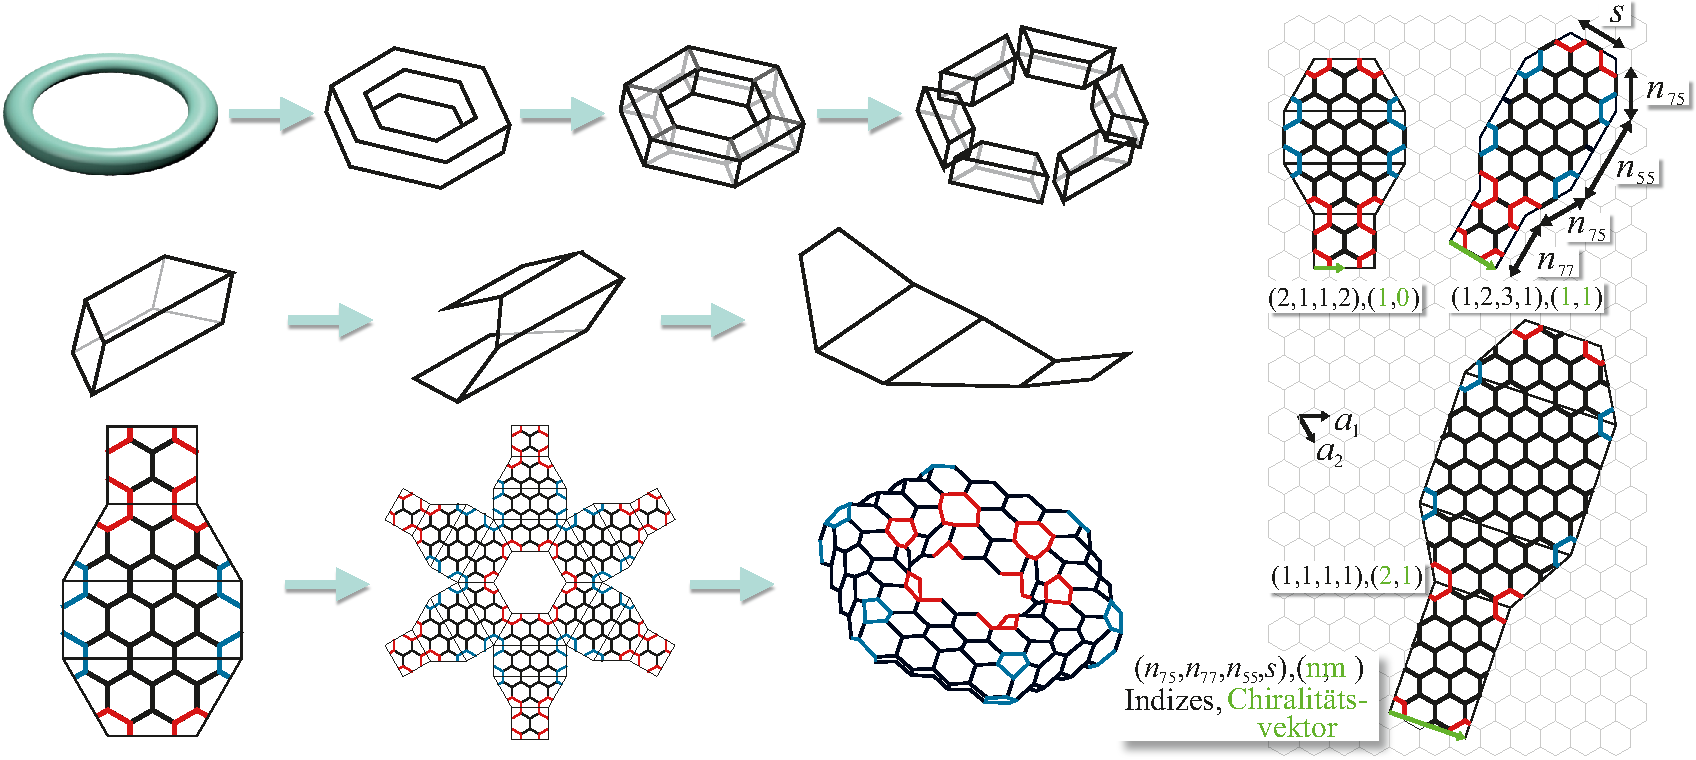
\includegraphics[width=1.0\textwidth]{konstruktion}
	\captionsetup{figurewithin = chapter}
	\captionsetup{font=small, labelfont=bf}\caption[Konstruktionsschema von toroidalen Kohlenstoff-Nanoröhren mit fünf- und siebengliedrigen Ringen]{Konstruktionsschema von toroidalen Kohlenstoff-Nanoröhren mit fünf- und siebengliedrigen Ringen. Reproduziert mit Erlaubnis von Referenz \cite{beuerle2011optical}. Copyright 2011 John Wiley and Sons.}
\label{abb:tcntkonstruktion}
\end{figure}
\FloatBarrier
Eine eindeutige Definition dieser \acp{tcnt} erfolgt durch die Angabe eines Chiralitätsvektors $(n,m)$ und 4 weiterer Parameter $(n_{75},n_{77},n_{55},s)$ (Abbildung \ref{abb:tcntkonstruktion}, rechte Seite). Im Einzelnen geben die Parameter $n_{75}$, $n_{77}$ und $n_{55}$ den Abstand zwischen den Heptagonen und Pentagonen, Heptagonen und Heptagonen sowie Pentagonen und Pentagonen an. $n_{75}$ beschreibt damit die Breite der zugrunde liegenden \ac{cnt}, $n_{77}$ die Höhe der inneren Wand des polygonalen Prismas und $n_{55}$ die Höhe der äußeren Wand. Der Parameter $s$ gibt die Länge der einzelnen Segmente an. Im Gegensatz zu den \acp{cnt} zeigt der Chiralitätsvektor in diesem Schema in die Richtung der Röhrenachse und nicht senkrecht dazu. Die fünf- und siebengliedrigen Ringe liegen bei diesem Konstruktionsschema unter- und oberhalb des Äquators der entsprechenden \ac{tcnt}. Im weiteren Verlauf werden diese Strukturen als \glqq Chuang-Strukturtyp\grqq{} bezeichnet. Die untersuchten Strukturen besitzen die Parameter $(2,1,1,s=1,\dots,9),(1,0)$ (\textit{armchair}) und $(1,2,2,s=1,\dots,5),(1,1)$ (\textit{zigzag}) und ihnen liegen $(4,4)$ \textit{armchair}- und $(7,0)$ \textit{zigzag}-\acp{cnt} zugrunde.\\

Die von Dunlap vorgeschlagene Verknüpfung von $(n,n)$-\textit{armchair}- und $(2n,0)$-\textit{zigzag}-\acp{cnt} führt zu einer alternativen \ac{tcnt}-Struktur. Das grundsätzliche Vorgehen ist in Abbildung \ref{abb:dunlap-konstruktion} gezeigt. Hier wird die $(n,n)$-\ac{cnt} in einem Winkel von etwa 30$^\circ$ geschnitten und mit einer entsprechenden $(2n,0)$-\ac{cnt} verknüpft, wodurch ebenfalls fünf- und siebengliedrige Kohlenstoffringe eingeführt werden. Im Unterschied zum \glqq Chuang-Strukturtyp\grqq{} liegen diese jedoch auf dem Äquator. Durch die Kombination von jeweils sechs \textit{armchair}- und \textit{zigzag}-\ac{cnt}-Einheiten, wie sie auf der rechten Seite in Abbildung \ref{abb:dunlap-konstruktion} dargestellt sind, resultiert eine \textit{D}$_{6\text{h}}$-symmetrische \ac{tcnt}. Das gemeinsame Vorhandensein von \textit{armchair}- und \textit{zigzag}-\acp{cnt} in diesem \glqq Dunlap-Strukturtyp\grqq{} lässt andere elektronische und magnetische Eigenschaften vermuten. Es werden zwei unterschiedliche Serien betrachtet: $2,\dots,7(4,4),1(8,0)$ mit zunehmender Länge der \textit{armchair}-\ac{cnt} und der kürzest möglichen Länge der \textit{zigzag}-\ac{cnt} (\glqq Dunlap-\textit{armchair}-\textit{zigzag} 1\grqq{}) und die Strukturen $2(4,4),2(8,0)$; $3(4,4),2(8,0)$; $2(4,4),3(8,0)$; $3(4,4),3(8,0)$ bei denen die Länge der \textit{zigzag}-\ac{cnt} ebenfalls zunimmt (\glqq Dunlap-\textit{armchair}-\textit{zigzag} 2\grqq{}).
\begin{figure}[ht!]
	\centering
	\includegraphics[width=1.0\textwidth]{dunlap-konstruktion}
	\captionsetup{figurewithin = chapter}
	\captionsetup{font=small, labelfont=bf}\caption[Verknüpfung von $(n,n)$-\textit{armchair}- und $(2n,0)$-\textit{zigzag}-\acp{cnt}]{Verknüpfung von \textit{armchair}- und \textit{zigzag}-Kohlenstoff-Nanoröhren (\acp{cnt}) nach Dunlap\supercite{dunlap1992connecting}. Die $(n,n)$-\ac{cnt} wird dabei in einem Winkel von etwa 30$^\circ$ geschnitten und mit einer entsprechenden $(2n,0)$-\ac{cnt} verknüpft (oben links). Die daraus resultierenden fünf- und siebengliedrigen Kohlenstoffringe sind in blau und rot eingezeichnet. Auf der rechten Seite sind unterschiedlich lange $(n,n)$- und $(2n,0)$-\ac{cnt}-Segmente dargestellt. Durch Kombination von jeweils sechs dieser Segmente werden \textit{D}$_{6\text{h}}$-symmetrische \acp{tcnt} erhalten.}
\label{abb:dunlap-konstruktion}
\end{figure}
\FloatBarrier

Für die \textit{polyhex}-\acp{tcnt} wurden $(4,4)$-\textit{armchair}- und $(7,0)$-\textit{zigzag}-Strukturen mit entsprechender Atomanzahl generiert. Eine Übersicht aller untersuchten Strukturen ist in der Tabelle \ref{tab:tcnt} gegeben und Abbildung \ref{abb:tcnttypen} zeigt für jeden darin vorkommenden Strukturtyp exemplarisch eine \ac{tcnt} mit optimierten Strukturparametern. Die Optimierung der Strukturparameter aller Verbindungen erfolgte unter Symmetrieausnutzung mit dem TPSS-Funktional\supercite{tao2003climbing}, der Basis def2-SVP\supercite{weigend2005balanced} sowie der entsprechenden Auxiliarbasis\supercite{weigend2006accurate}. Zusätzlich wurde Grimmes Dispersionskorrektur D3\supercite{grimme2010consistent,grimme2011effect} verwendet. Das \ac{marij}-Verfahren wurde sowohl bei der Optimierung\supercite{sierka2003fast} als auch bei der Berechnung der magnetischen Response\supercite{reiter2017calculation} ausgenutzt. Letztere wurde, sofern nicht explizit erwähnt, ebenfalls mit dem TPSS-Funktional und der Basis def2-SVP berechnet. Die eigentliche Berechnung der Ringströme erfolgte mit \ac{gimic}\supercite{juselius2004calculation,taubert2011calculation,fliegl2011gauge,sundholm2016calculations}.

\begin{table}[htbp!]
  \centering
\captionsetup{tablewithin = chapter}
\captionsetup{font=small, labelfont=bf}
\captionabove[Eigenschaften von untersuchten \acp{tcnt}]{Anzahl der Kohlenstoffatome ($N_\text{C}$), Strukturparameter, Symmetrie, HOMO-LUMO-Gap und Gesamtringstrom in unterschiedlichen toroidalen Kohlenstoff-Nanoröhren.}
\resizebox{\textwidth}{!}{%
    \begin{tabular}{lccccS[table-format = 3.1]}
    \hline \hline
    Strukturtyp & $N_\text{C}$ & Struktur- & Symmetrie & HOMO-LUMO-Gap & \text{Ringstrom} \\
          &       & Parameter      &       & eV    & \text{\;\;\;\;nA/T} \\
    \hline
    \textit{polyhex}-\textit{armchair}& 480   & (4,4),($-$30,30) & \textit{C}$_{30\text{v}}$  & 0.20  & 84.4 \\
    \textit{polyhex}-\textit{armchair}& 576   & (4,4),($-$36,36) & \textit{C}$_{36\text{v}}$  & 0.18  & 112.8 \\
    \textit{polyhex}-\textit{armchair}& 672   & (4,4),($-$42,42) & \textit{C}$_{42\text{v}}$  & 0.14  & 143.4 \\
    \textit{polyhex}-\textit{armchair}& 768   & (4,4),($-$48,48) & \textit{C}$_{48\text{v}}$  & 0.13  & 171.3 \\
    \textit{polyhex}-\textit{armchair}& 864   & (4,4),($-$54,54) & \textit{C}$_{54\text{v}}$  & 0.11  & 200.7 \\
    \textit{polyhex}-\textit{armchair}& 960   & (4,4),($-$60,60) & \textit{C}$_{60\text{v}}$  & 0.10  & 235.7 \\
          &       &       &       &       &  \\
    \textit{polyhex}-\textit{zigzag} & 588   & (7,0),($-$21,42) & \textit{D}$_{21\text{h}}$  & 0.16  & 9.5 \\
    \textit{polyhex}-\textit{zigzag} & 756   & (7,0),($-$27,54) & \textit{D}$_{27\text{h}}$  & 0.31  & 1.7 \\
    \textit{polyhex}-\textit{zigzag} & 924   & (7,0),($-$33,66) & \textit{D}$_{33\text{h}}$  & 0.17  & 1.1 \\
          &       &       &       &       &  \\
    Chuang-\textit{armchair}& 192   & (2,1,1,1),(1,0) & \textit{D}$_{6\text{h}}$   & 1.33  & $\num{-3.5}$ \\
    Chuang-\textit{armchair}& 288   & (2,1,1,2),(1,0) & \textit{D}$_{6\text{h}}$   & 0.32  & $\num{-0.6}$ \\
    Chuang-\textit{armchair}& 384   & (2,1,1,3),(1,0) & \textit{D}$_{6\text{h}}$   & 0.29  & $\num{-2.4}$ \\
    Chuang-\textit{armchair}& 480   & (2,1,1,4),(1,0) & \textit{D}$_{6\text{h}}$   & 0.52  & $\num{-2.5}$ \\
    Chuang-\textit{armchair}& 576   & (2,1,1,5),(1,0) & \textit{D}$_{6\text{h}}$   & 0.04  & 57.7 \\
    Chuang-\textit{armchair}& 672   & (2,1,1,6),(1,0) & \textit{D}$_{6\text{h}}$   & 0.40  & $\num{-2.2}$ \\
    Chuang-\textit{armchair}& 768   & (2,1,1,7),(1,0) & \textit{D}$_{6\text{h}}$   & 0.23  & $\num{-3.8}$ \\
    Chuang-\textit{armchair}& 864   & (2,1,1,8),(1,0) & \textit{D}$_{6\text{h}}$   & 0.09  & $\num{-1.9}$ \\
    Chuang-\textit{armchair}& 960   & (2,1,1,9),(1,0) & \textit{D}$_{6\text{h}}$   & 0.31  & $\num{-2.7}$ \\
          &       &       &       &       &  \\
    Chuang-\textit{zigzag} & 252   & (1,2,2,1),(1,1) & \textit{D}$_{6\text{h}}$   & 0.26  & $\num{-8.4}$ \\
    Chuang-\textit{zigzag} & 420   & (1,2,2,2),(1,1) & \textit{D}$_{6\text{h}}$   & 0.07  & $\num{-94.0}$ \\
    Chuang-\textit{zigzag} & 588   & (1,2,2,3),(1,1) & \textit{D}$_{6\text{h}}$   & 0.25  & $\num{-12.9}$ \\
    Chuang-\textit{zigzag} & 756   & (1,2,2,4),(1,1) & \textit{D}$_{6\text{h}}$   & 0.36  & $\num{-3.5}$ \\
    Chuang-\textit{zigzag} & 924   & (1,2,2,5),(1,1) & \textit{D}$_{6\text{h}}$   & 0.33  & $\num{-1.5}$ \\
          &       &       &       &       &  \\
    Dunlap-\textit{armchair}-\textit{zigzag} 1& 480   & 2(4,4),1(8,0) & \textit{D}$_{6\text{h}}$   & 0.16  & 73.7 \\
    Dunlap-\textit{armchair}-\textit{zigzag} 1& 576   & 3(4,4),1(8,0) & \textit{D}$_{6\text{h}}$   & 0.18  & 117.8 \\
    Dunlap-\textit{armchair}-\textit{zigzag} 1& 672   & 4(4,4),1(8,0) & \textit{D}$_{6\text{h}}$   & 0.08  & $\num{-94.6}$ \\
    Dunlap-\textit{armchair}-\textit{zigzag} 1& 768   & 5(4,4),1(8,0) & \textit{D}$_{6\text{h}}$   & 0.19  & 149.0 \\
    Dunlap-\textit{armchair}-\textit{zigzag} 1& 864   & 6(4,4),1(8,0) & \textit{D}$_{6\text{h}}$   & 0.08  & 172.3 \\
    Dunlap-\textit{armchair}-\textit{zigzag} 1& 960   & 7(4,4),1(8,0) & \textit{D}$_{6\text{h}}$   & 0.10  & 177.6 \\
          &       &       &       &       &  \\
    Dunlap-\textit{armchair}-\textit{zigzag} 2& 672   & 2(4,4),2(8,0) & \textit{D}$_{6\text{h}}$   & 0.09  & 94.6 \\
    Dunlap-\textit{armchair}-\textit{zigzag} 2& 768   & 3(4,4),2(8,0) & \textit{D}$_{6\text{h}}$   & 0.12  & 119.2 \\
    Dunlap-\textit{armchair}-\textit{zigzag} 2& 864   & 2(4,4),3(8,0) & \textit{D}$_{6\text{h}}$   & 0.03  & 101.1 \\
    Dunlap-\textit{armchair}-\textit{zigzag} 2& 960   & 3(4,4),3(8,0) & \textit{D}$_{6\text{h}}$   & 0.07  & $\num{-4.1}$ \\
    \end{tabular}}%
  \label{tab:tcnt}%
\end{table}%
\vfill
\FloatBarrier
\newpage

\begin{figure}[ht!]
	\centering
	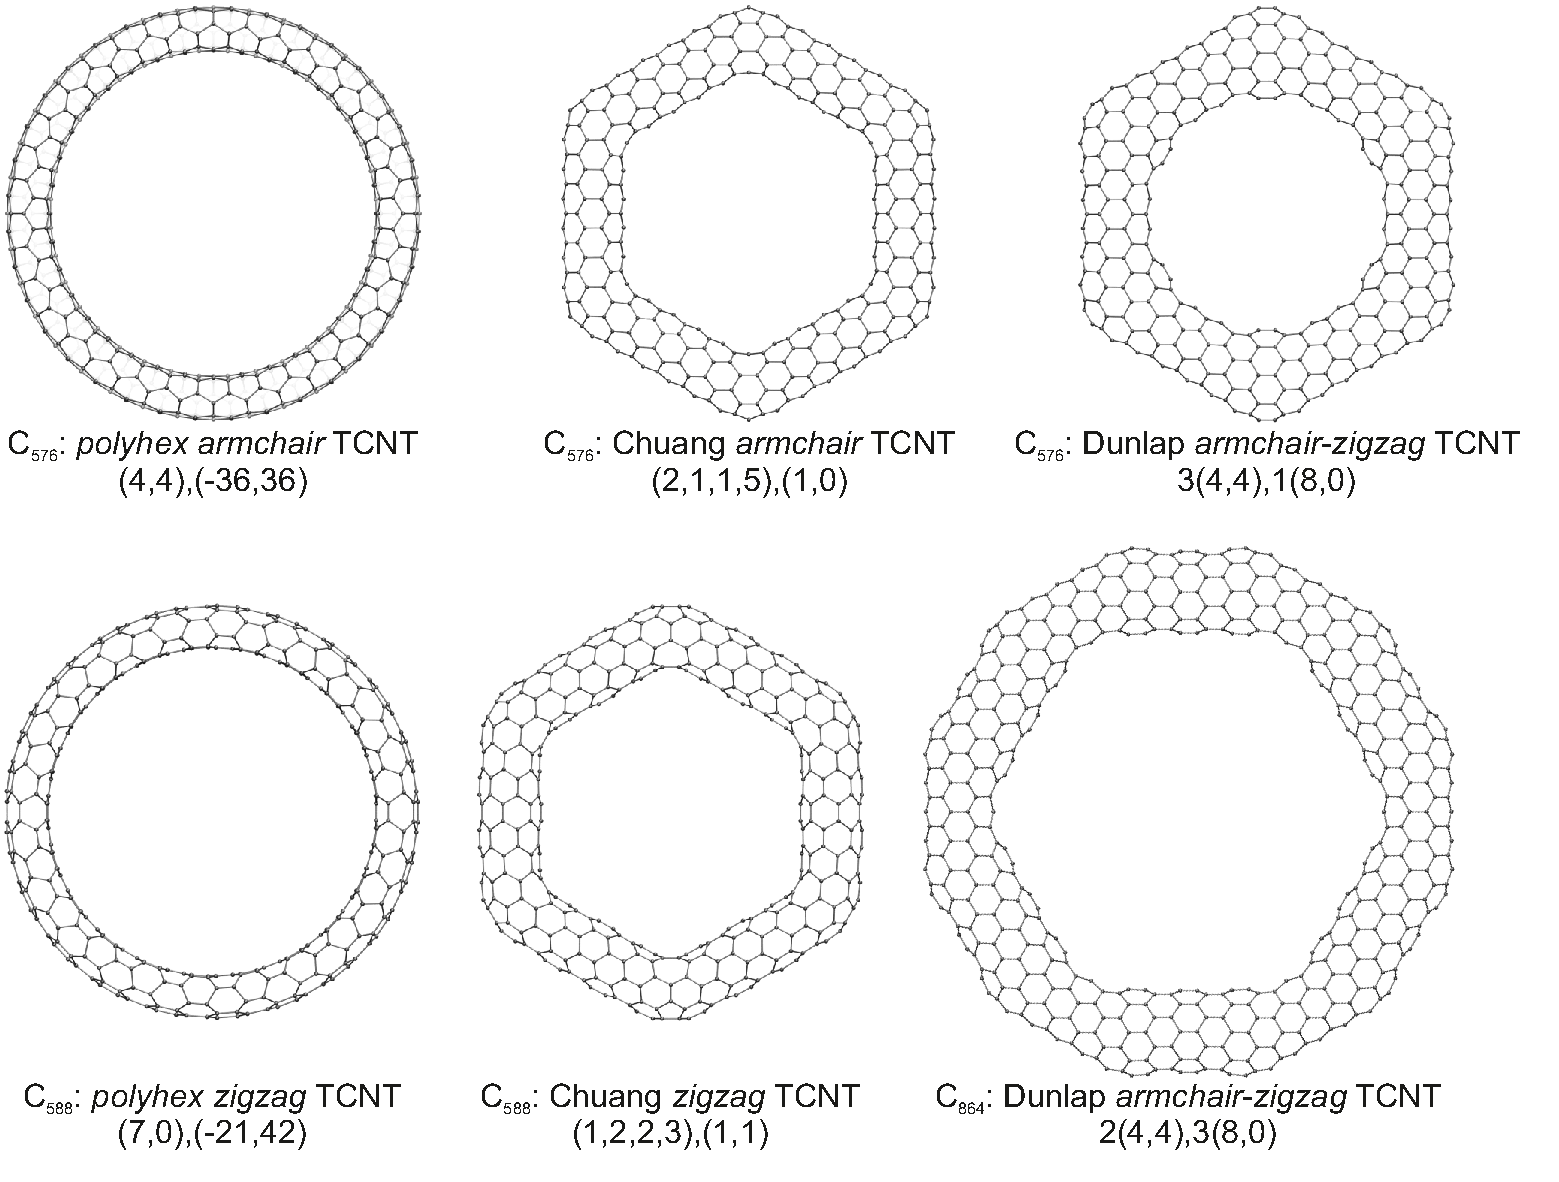
\includegraphics[width=1.0\textwidth]{tcnttypen}
	\captionsetup{figurewithin = chapter}
	\captionsetup{font=small, labelfont=bf}\caption[Strukturtypen von toroidalen Kohlenstoff-Nanoröhren]{Unterschiedliche Strukturtypen von toroidalen Kohlenstoff-Nanoröhren (\acp{tcnt}) mit def2-SVP/TPSS-optimierten Strukturparametern.}
\label{abb:tcnttypen}
\end{figure}

\subsection{Stabilität}
In Abbildung \ref{abb:tcntbindungsenergie} ist für jede der berechneten Strukturen die Bindungsenergie pro Kohlenstoffatom aufgetragen. Es zeigt sich, dass bei den hier betrachteten Ringgrößen die \textit{polyhex}-\acp{tcnt} energetisch gegenüber den anderen Strukturtypen deutlich benachteiligt sind. Zudem kommt es bei der Optimierung der Strukturparameter für diese \acp{tcnt} zu einer Verformung des Nanoröhrenquerschnitts. Aufgrund des vergleichsweise kleinen Torusdurchmessers werden auf der Innenseite zu kurze und auf der Außenseite zu lange Kohlenstoffabstände erhalten. Durch die Verformung zu einem elliptischen Röhrenquerschnitt wird die Spannung im Ring reduziert. Aus Abbildung \ref{abb:tcntbindungsenergie} ist aber ebenfalls ersichtlich, dass die Benachteiligung der \textit{polyhex}-\acp{tcnt} mit zunehmender Größe schnell abnimmt und für große Ringe vermutlich verschwindet. Somit können die betrachteten Systeme als Modellverbindungen für die großen, thermodynamisch stabilen Analoga angesehen und ihre elektronischen und magnetischen Eigenschaften auf diese extrapoliert werden.

\begin{figure}[ht!]
	\centering
	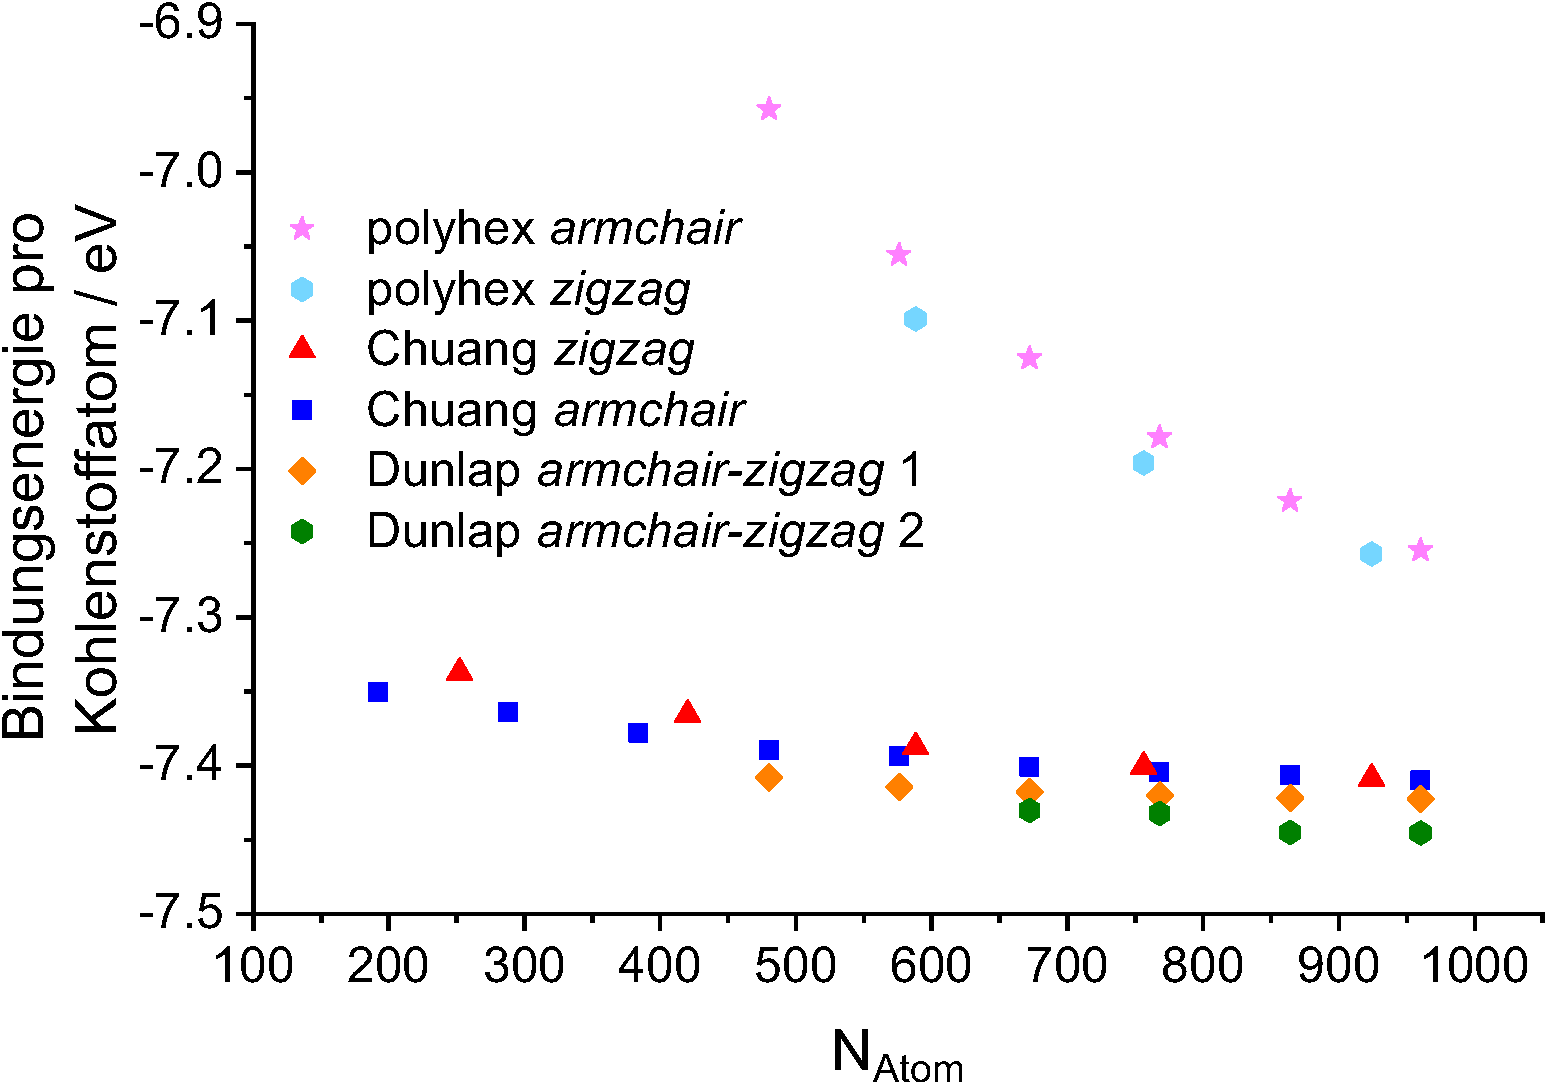
\includegraphics[width=0.68\textwidth]{tcntbindungsenergie}
	\captionsetup{figurewithin = chapter}
	\captionsetup{font=small, labelfont=bf}\caption[Bindungsenergie toroidaler Kohlenstoff-Nanoröhren]{Bindungsenergie pro Kohlenstoffatom in unterschiedlichen Strukturtypen toroidaler Kohlenstoff-Nanoröhren.}
\label{abb:tcntbindungsenergie}
\end{figure}

\subsection{Ringströme}

Die berechneten Ringströme für alle untersuchten Systeme sind zusammen mit den HOMO-LUMO-Gaps in Tabelle \ref{tab:tcnt} aufgelistet. Zusätzlich ist der Zusammenhang des Gesamtringstroms mit der Systemgröße $N_\textrm{C}$ in Abbildung \ref{abb:tcntcurvssize} und mit dem HOMO-LUMO-Gap in Abbildung \ref{abb:tcntcurvsgap} aufgetragen. Wie der Tabelle zu entnehmen ist, besitzen alle \textit{polyhex}-\textit{armchair}-\acp{tcnt} einen großen diatropischen Gesamtringstrom und können damit als aromatisch klassifiziert werden. Dieser Gesamtringstrom setzt sich aus den gegenläufigen diatropischen und paratropischen Beiträgen zusammen und steigt weitgehend linear mit der Systemgröße von \unit[84.4]{nA/T} für C$_{480}$ auf \unit[235.7]{nA/T} für C$_{960}$ an (siehe auch Abbildung \ref{abb:tcntcurvssize}). Im Gegensatz dazu sind die diatropischen und paratropischen Beiträge in den \textit{polyhex}-\textit{zigzag}-\acp{tcnt} in etwa von derselben Größe und der Gesamtringstrom verschwindet nahezu vollkommen. Dieser Befund passt gut zur Einteilung in metallische (mit Gesamtringstrom) und isolierende (ohne Gesamtringstrom) \acp{tcnt} nach Referenz \cite{zhang2005electronic}. Für die anderen Strukturtypen (Chuang und Dunlap) sind keine solch einfachen Regeln zur Einteilung bekannt. Interessanterweise besitzen die betrachteten \glqq Chuang-\textit{armchair}-\acp{tcnt}\grqq{}, welche aus metallischen \acp{cnt} aufgebaut sind, mit Ausnahme von C$_{576}$ ebenfalls keinen Gesamtringstrom. Im C$_{576}$ ist dieser mit \unit[57.7]{nA/T} auch nur etwa halb so groß wie in der entsprechenden \textit{polyhex}-\ac{tcnt} mit derselben Atomanzahl (\unit[112.8]{nA/T}). Ein ähnliches Bild ergibt sich für die entsprechenden \glqq Chuang \textit{zigzag}-\acp{tcnt}\grqq{}. Hier wird ebenfalls nur eine Verbindung mit großem Ringstrom erhalten. Diese besitzt im Vergleich zu den anderen Strukturen jedoch einen paratropischen Gesamtringstrom und ist damit als antiaromatisch einzuordnen. Die Serie \glqq Dunlap-\textit{armchair}-\textit{zigzag} 1\grqq{} zeigt ein ähnliches Verhalten wie die \textit{polyhex}-\textit{armchair}-Verbindungen derselben Größe. Alle Verbindungen dieses Typs besitzen ebenfalls einen großen Gesamtringstrom. Im Allgemeinen fällt dieser jedoch etwas kleiner aus als in den \textit{polyhex}-Strukturen. Weiterhin steigt dieser nicht linear mit der Systemgröße an, denn die Zunahme des Gesamtringstroms wird mit steigender Atomanzahl geringer. Unerwarteterweise fällt die Verbindung C$_{672}$ mit einem paratropischen Gesamtringstrom von \unit[$-$94.6]{nA/T} aus der Reihe, alle anderen Verbindungen dieses Strukturtyps besitzen diatropische Gesamtringströme. An dieser Stelle kann jedoch festgehalten werden, dass das kurze nichtmetallische \textit{zigzag}-\ac{cnt}-Segment den Gesamtringstrom in diesen Verbindungen nicht aufhebt. In der zweiten Serie \glqq Dunlap-\textit{armchair}-\textit{zigzag} 2\grqq{} nimmt die Länge dieses Segments zu, was zu etwas niedrigeren Gesamtringströmen im Vergleich zur ersten Serie führt. Für C$_{960}$ verschwindet dieser vollkommen. \\

\begin{figure}[ht!]
	\centering
	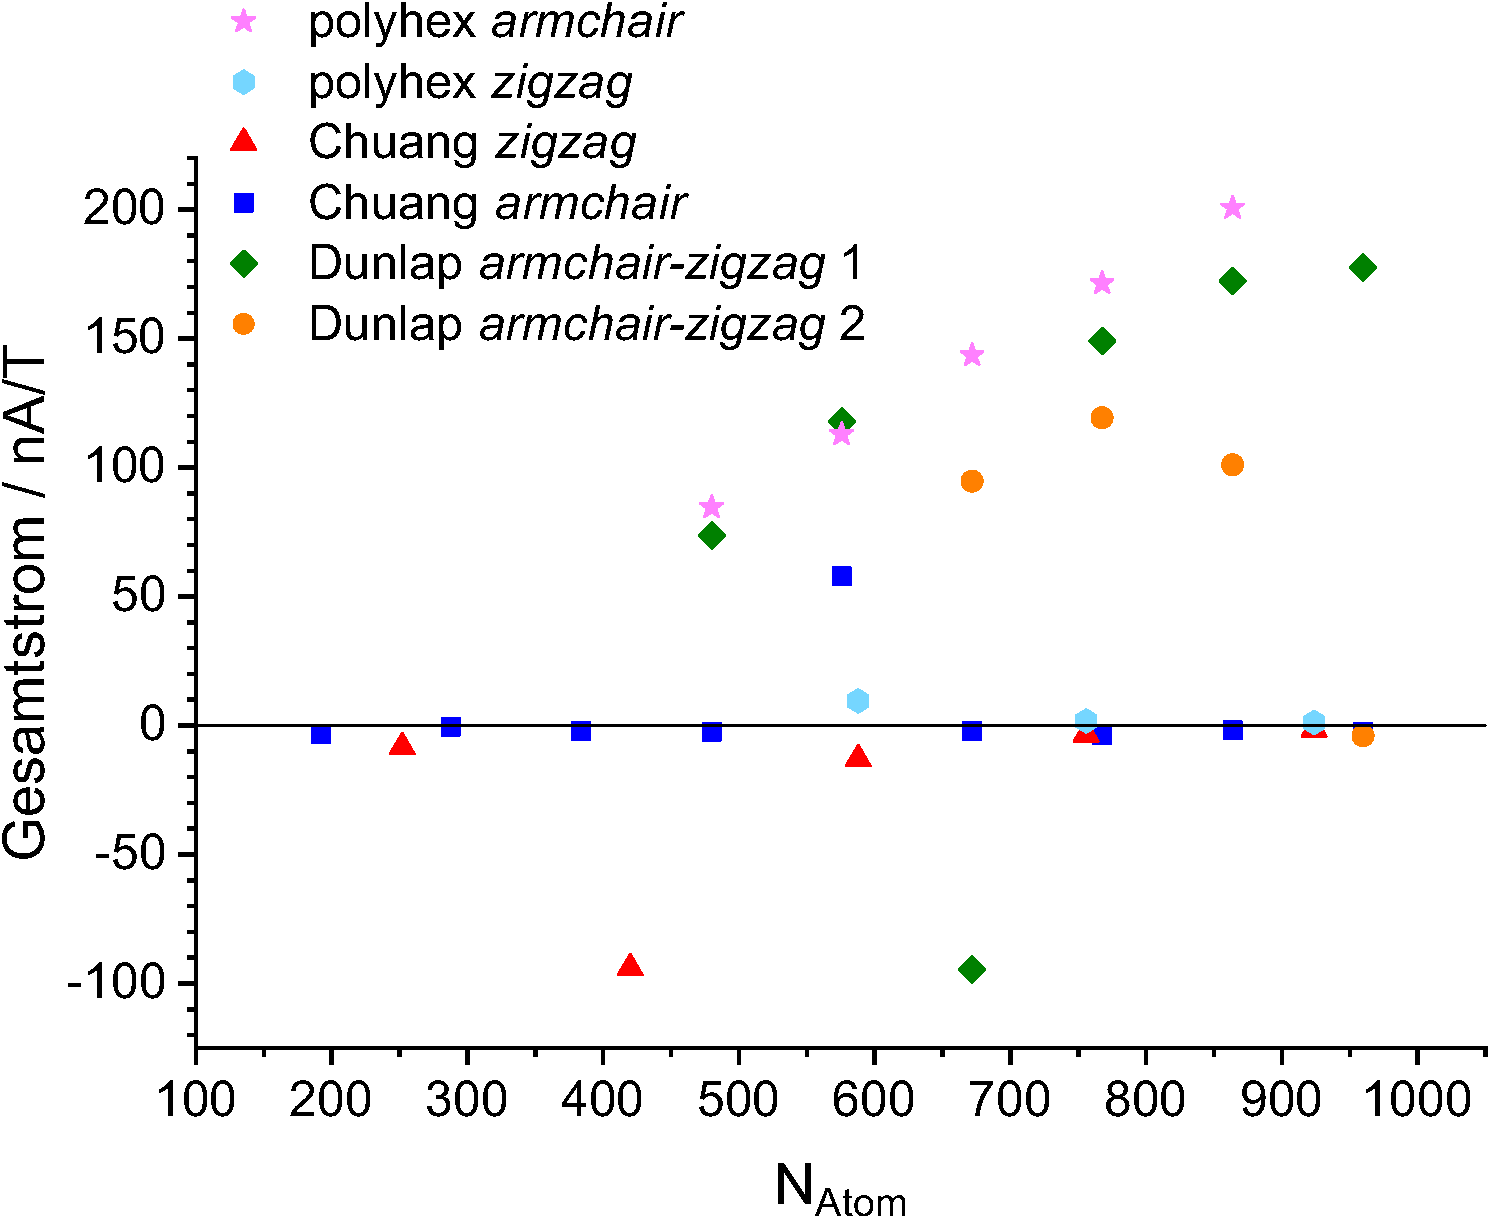
\includegraphics[width=0.68\textwidth]{tcntcurvssize}
	\captionsetup{figurewithin = chapter}
	\captionsetup{font=small, labelfont=bf}\caption[Zusammenhang zwischen Gesamtringstrom und Systemgröße]{Zusammenhang zwischen Gesamtringstrom und Systemgröße.}
\label{abb:tcntcurvssize}
\end{figure}
\vfill
\FloatBarrier
\newpage

\begin{figure}[ht!]
	\centering
	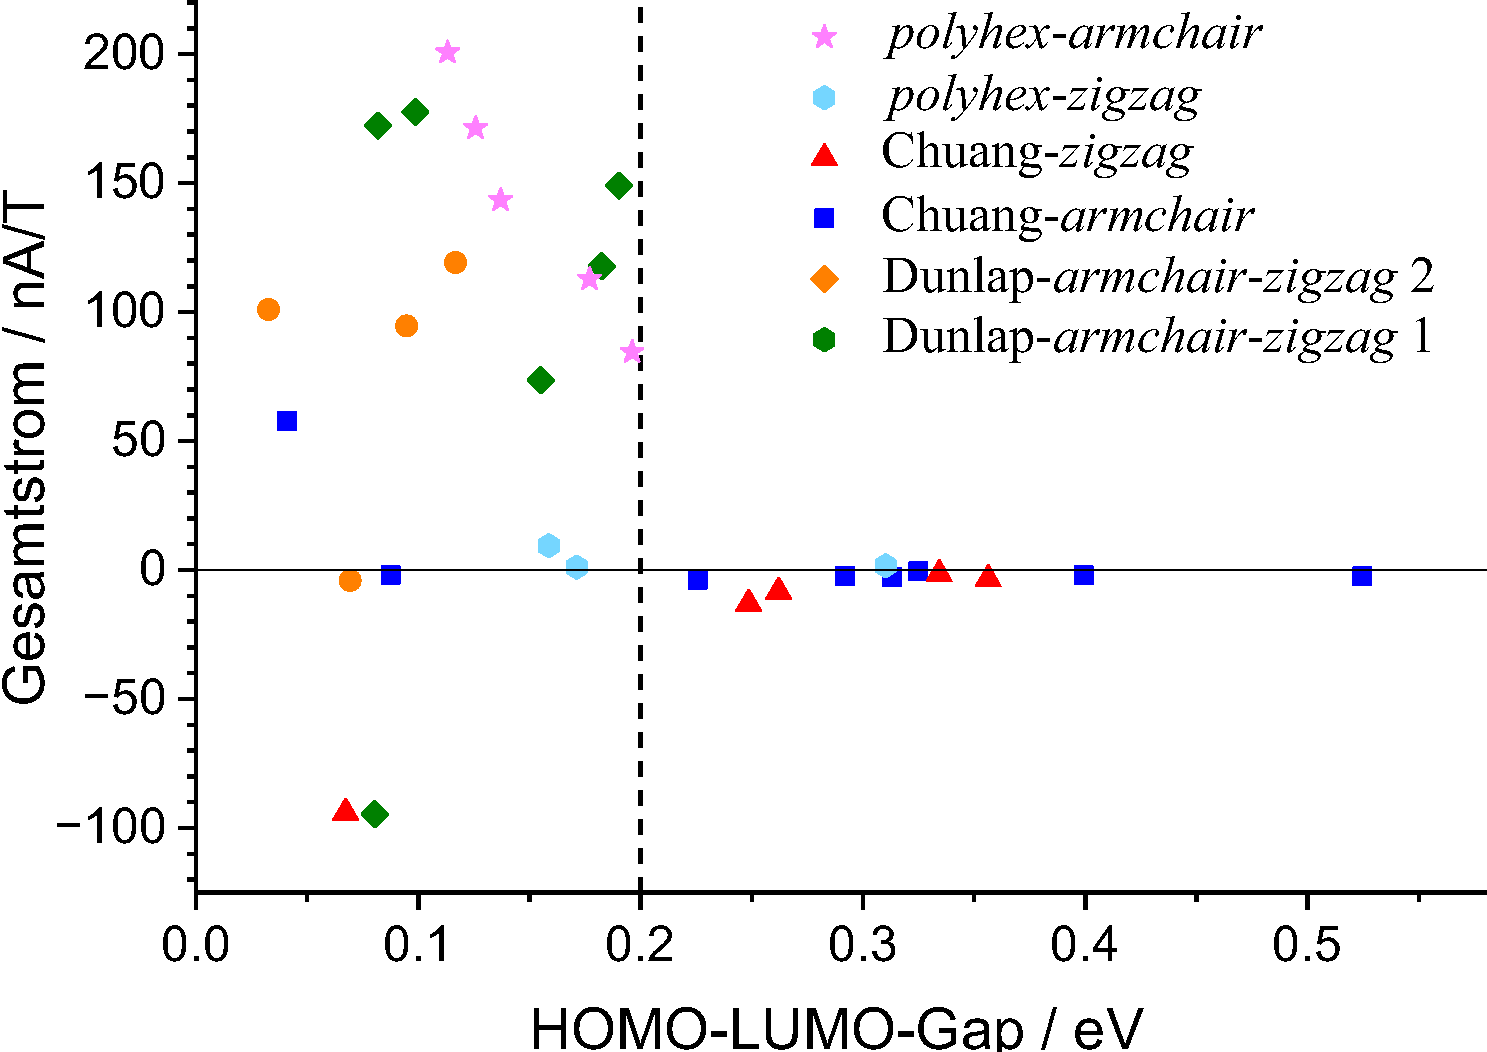
\includegraphics[width=0.68\textwidth]{tcntcurvsgap}
	\captionsetup{figurewithin = chapter}
	\captionsetup{font=small, labelfont=bf}\caption[Zusammenhang zwischen Gesamtringstrom und HOMO-LUMO-Gap]{Zusammenhang zwischen Gesamtringstrom und HOMO-LUMO-Gap. Alle in der vorliegenden Arbeit untersuchten Verbindungen, welche einen Gesamtringstrom aufweisen, besitzen eine HOMO-LUMO-Gap von $\leq$ \unit[0.2]{eV}.}
\label{abb:tcntcurvsgap}
\end{figure}
\FloatBarrier

Die bisherigen Rechnungen wurden ausschließlich mit dem TPSS-Funktional durchgeführt. Im Folgenden wird die Abhängigkeit der Ergebnisse vom verwendeten Funktional exemplarisch für die Serie \glqq Dunlap-\textit{armchair}-\textit{zigzag} 1\grqq{} untersucht, wobei die mit dem TPSS-Funktional optimierten Strukturparameter verwendet wurden. Eine graphische Darstellung der Ergebnisse ist in Abbildung \ref{abb:tcntfunktional} gezeigt. 

\begin{figure}[ht!]
	\centering
	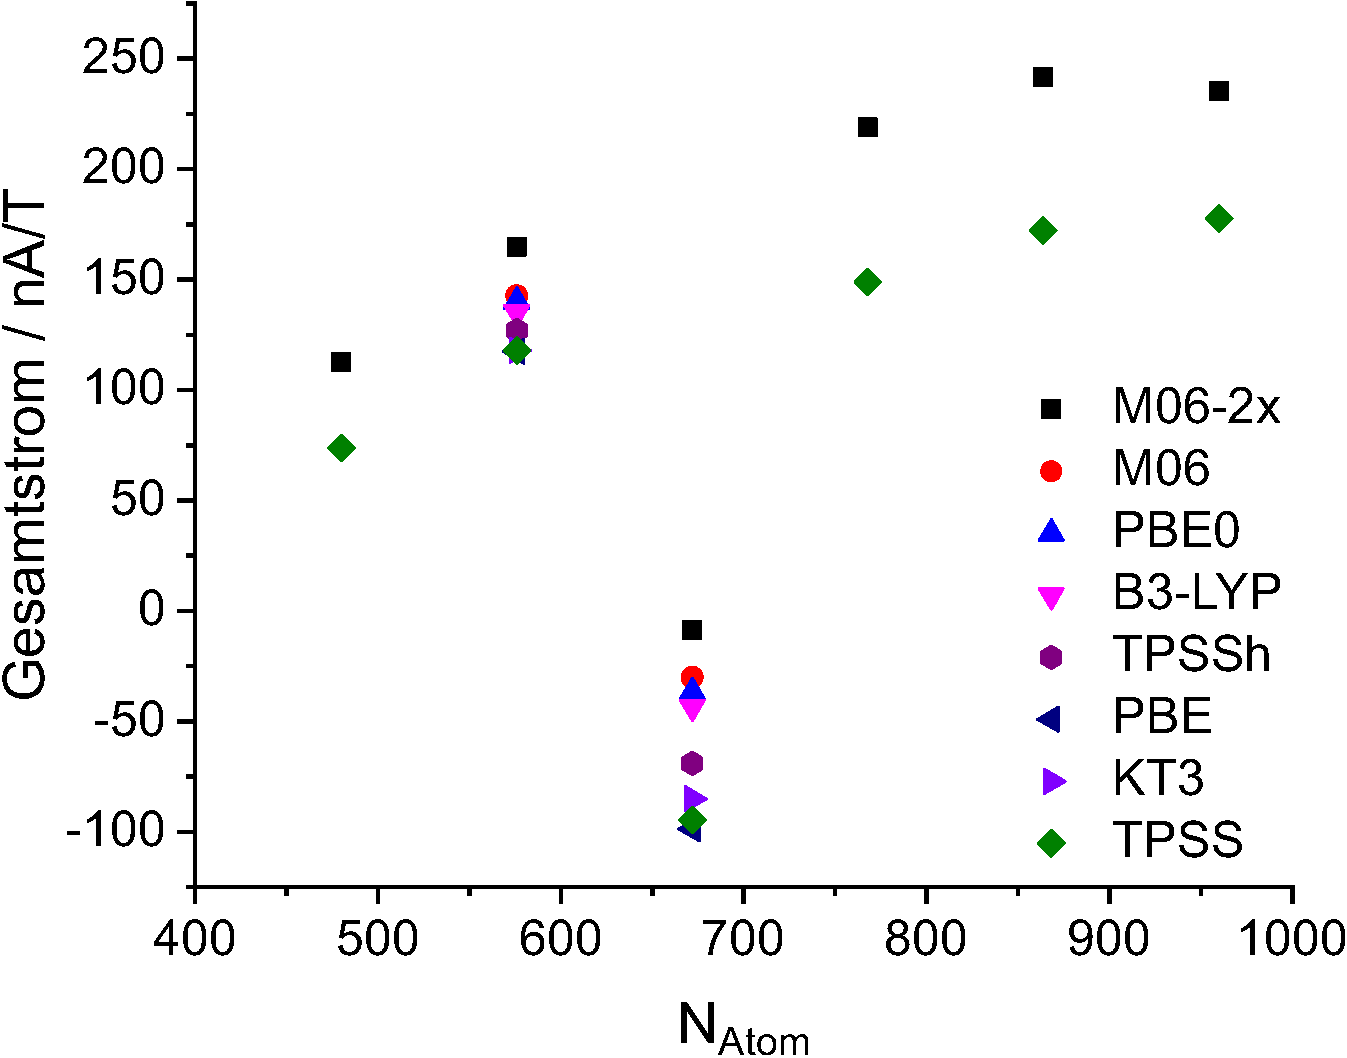
\includegraphics[width=0.68\textwidth]{tcntfunktional}
	\captionsetup{figurewithin = chapter}
	\captionsetup{font=small, labelfont=bf}\caption[Funktionaleinflüsse auf Ringströme]{Einflüsse unterschiedlicher Dichtefunktionale (mit variierendem Hartree-Fock-
Austausch) auf den Gesamtringstrom in der Serie \glqq Dunlap-\textit{armchair}-\textit{zigzag} 1\grqq{}.}
\label{abb:tcntfunktional}
\end{figure}
\FloatBarrier

Der Gesamtringstrom aller Verbindungen wurde dafür erneut mit dem M06-2x-Funktional\supercite{zhao2008m06} berechnet, welches 54 \% Hartree-Fock-Austausch beinhaltet. Für die beiden \acp{tcnt} C$_{576}$ und C$_{672}$ dieser Serie erfolgte zusätzlich die Berechnung mit den Funktionalen KT3\supercite{keal2004semiempirical}, PBE\supercite{perdew1996generalized}, TPSSh\supercite{staroverov2003comparative}, B3-LYP\supercite{becke1993density,lee1988development,stephens1994ab}, PBE0\supercite{adamo1999toward} und M06\supercite{zhao2008m06}. Der Vergleich zwischen TPSS und M06-2x zeigt, dass es mit dem Hybridfunktional zu einem allgemeinen Anstieg des Gesamtringstroms kommt. Der Trend innerhalb der Serie bleibt dabei jedoch erhalten. Aus den Berechnungen der anderen Funktionale kann ein nahezu linearer Anstieg des Gesamtringstroms mit zunehmenden Hartree-Fock-Austausch beobachtet werden.

\bigskip
In den beiden Abbildungen \ref{abb:homolumoarmchair} und \ref{abb:homolumozigzag} sind die HOMOs und LUMOs für ausgewählte Verbindungen der einzelnen Strukturtypen gezeigt. Diese sind in allen Fällen weitgehend über den gesamten Torus delokalisiert, was jedoch bereits alleine aus Symmetriegründen so sein muss. Bei den fünf- und siebengliedrige Kohlenstoffringe beinhaltenden \acp{tcnt} ist häufig eine leichte Lokalisierung an den pentagonalen und heptagonalen Einheiten zu erkennen. Die Delokalisierung der Orbitale ist jedoch kein ausreichendes Kriterium für das Auftreten eines großen Gesamtringstroms. Wichtiger ist die geometrische und damit einhergehende elektronische Struktur der \acp{tcnt}. Die Auftragung des Gesamtringstroms gegen das berechnete HOMO-LUMO-Gap in Abbildung \ref{abb:tcntcurvsgap} zeigt, dass letzteres für alle Verbindungen mit großem Gesamtringstrom kleiner als \unit[0.2]{eV} ist. Dies ist demnach eine notwendige, aber nicht hinreichende Bedingung für das Auftreten eines Ringstromes, da ebenfalls Strukturen mit kleinem Gap aber ohne Gesamtringstrom auftreten. Insbesondere in den \textit{polyhex}-\textit{armchair}- und \glqq Dunlap-\textit{armchair}-\textit{zigzag} 1\grqq{} Strukturtypen treten große Ringströme auf. Beiden ist gemeinsam, dass sie (im Wesentlichen) aus metallischen \acp{cnt} aufgebaut sind. Dies trifft auch auf den \glqq Chuang-\textit{armchair}\grqq{} Strukturtyp zu, jedoch verschwindet der Gesamtringstrom hier in den meisten Fällen oder ist deutlich kleiner. Daraus kann die Schlussfolgerung gezogen werden, dass die Lage und Orientierung der Pentagone und Heptagone innerhalb der \acp{tcnt} ebenfalls einen Einfluss auf den Gesamtringstrom hat. Liegen diese innerhalb des Äquators, treten größere Gesamtringströme auf als wenn sie unter- und oberhalb des Äquators liegen. Weiterhin kann festgehalten werden, dass es insbesondere in den \textit{polyhex}-\textit{armchair}-\acp{tcnt} zu einem weitgehend linearen Anstieg des Gesamtringstroms mit zunehmender Systemgröße kommt. Dies legt die Vermutung nahe, dass diese Ringströme ebenfalls in deutlich größeren und damit thermodynamisch stabilen \textit{polyhex}-\acp{tcnt} auftreten.

\begin{figure}[ht!]
	\centering
	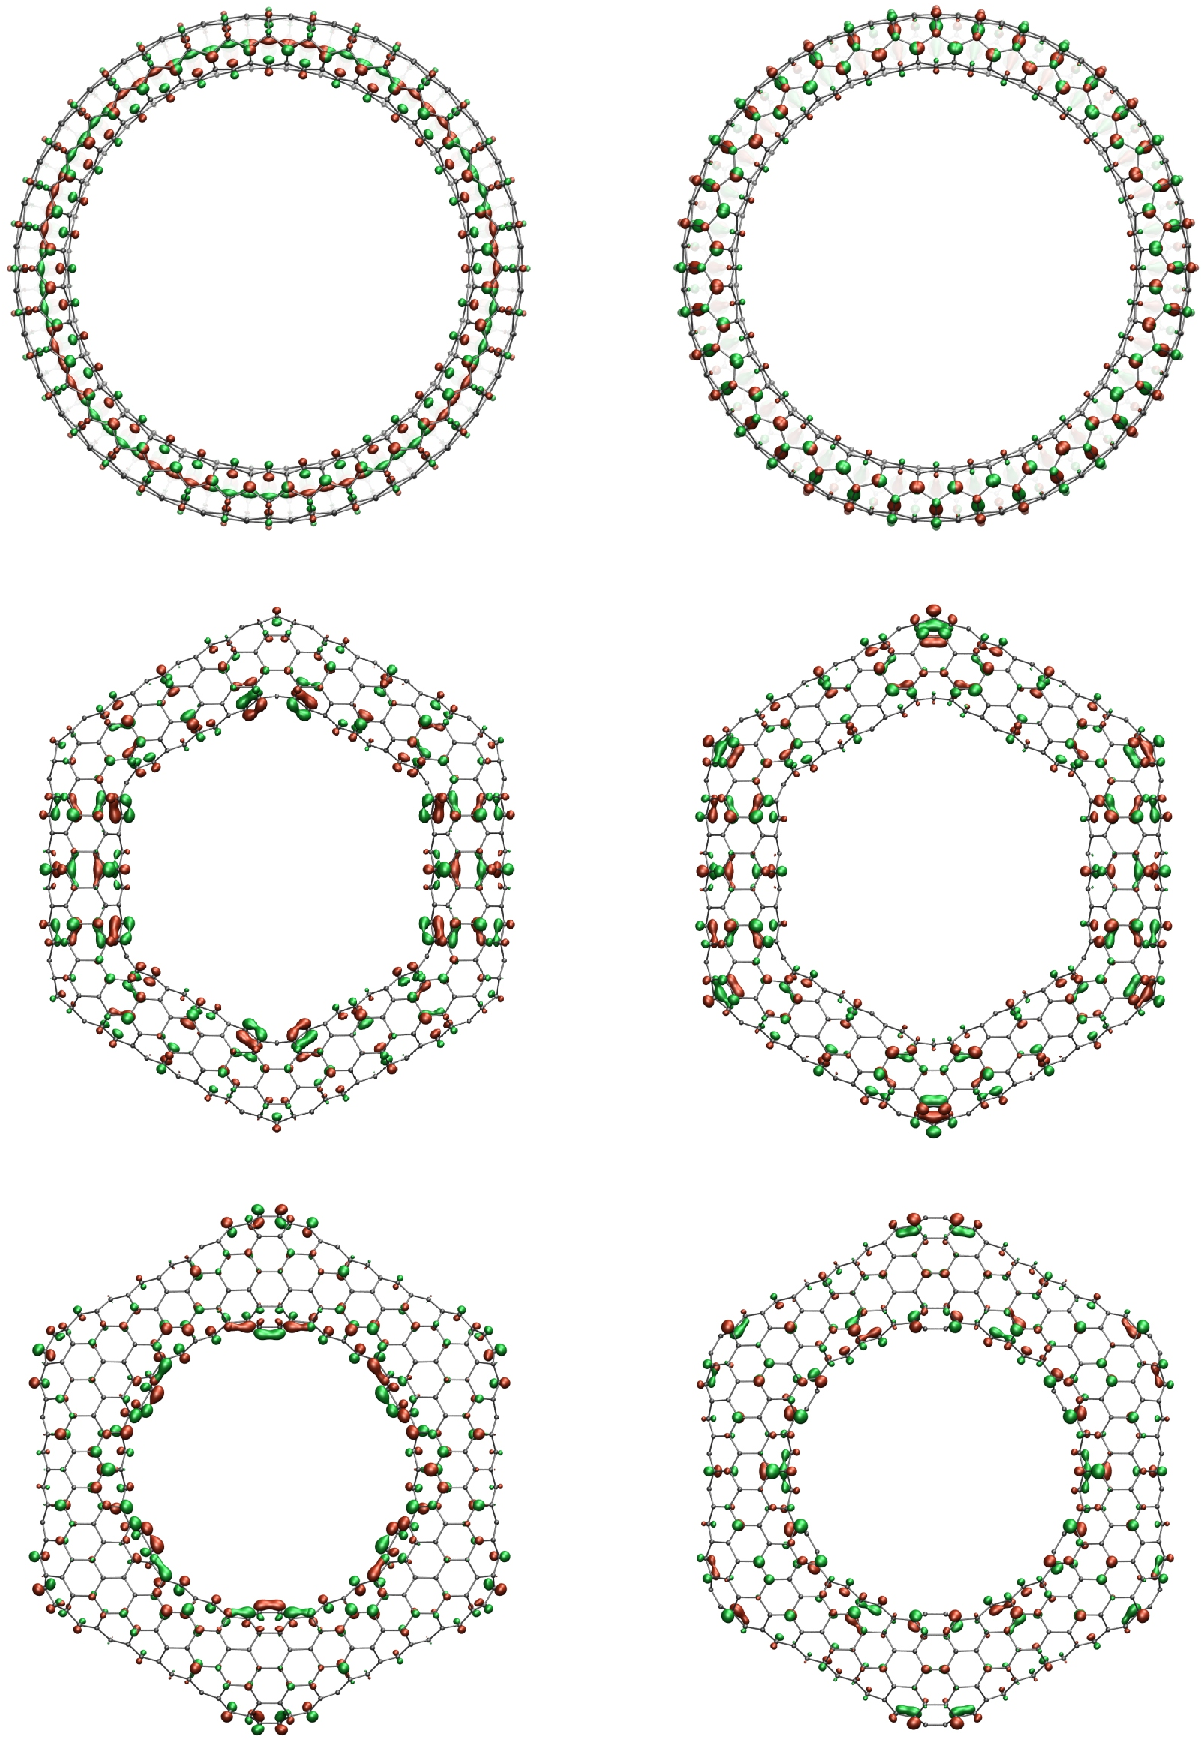
\includegraphics[width=0.92\textwidth]{homolumoarmchair}
	\captionsetup{figurewithin = chapter}
	\captionsetup{font=small, labelfont=bf}\caption[HOMO und LUMO von toroidalen Kohlenstoff-Nanoröhren 1]{HOMOs (links) und LUMOs (rechts) von toroidalen Kohlenstoff-Nanoröhren (\acp{tcnt}). C$_{576}$: \textit{polyhex}-\textit{armchair}-\ac{tcnt} (4,4),($-$36,36) (oben), C$_{576}$: Chuang-\textit{armchair}-\ac{tcnt} (2,1,1,5),(1,0) (Mitte) und C$_{576}$: Dunlap-\textit{armchair-zigzag}-\ac{tcnt} 3(4,4),1(8,0) (unten). Die Konturen von HOMO und LUMO wurden bei \unit[0.018]{a.u.} (grün) und \unit[$-$0.018]{a.u.} (rot) gezeichnet.}
\label{abb:homolumoarmchair}
\end{figure}

\begin{figure}[ht!]
	\centering
	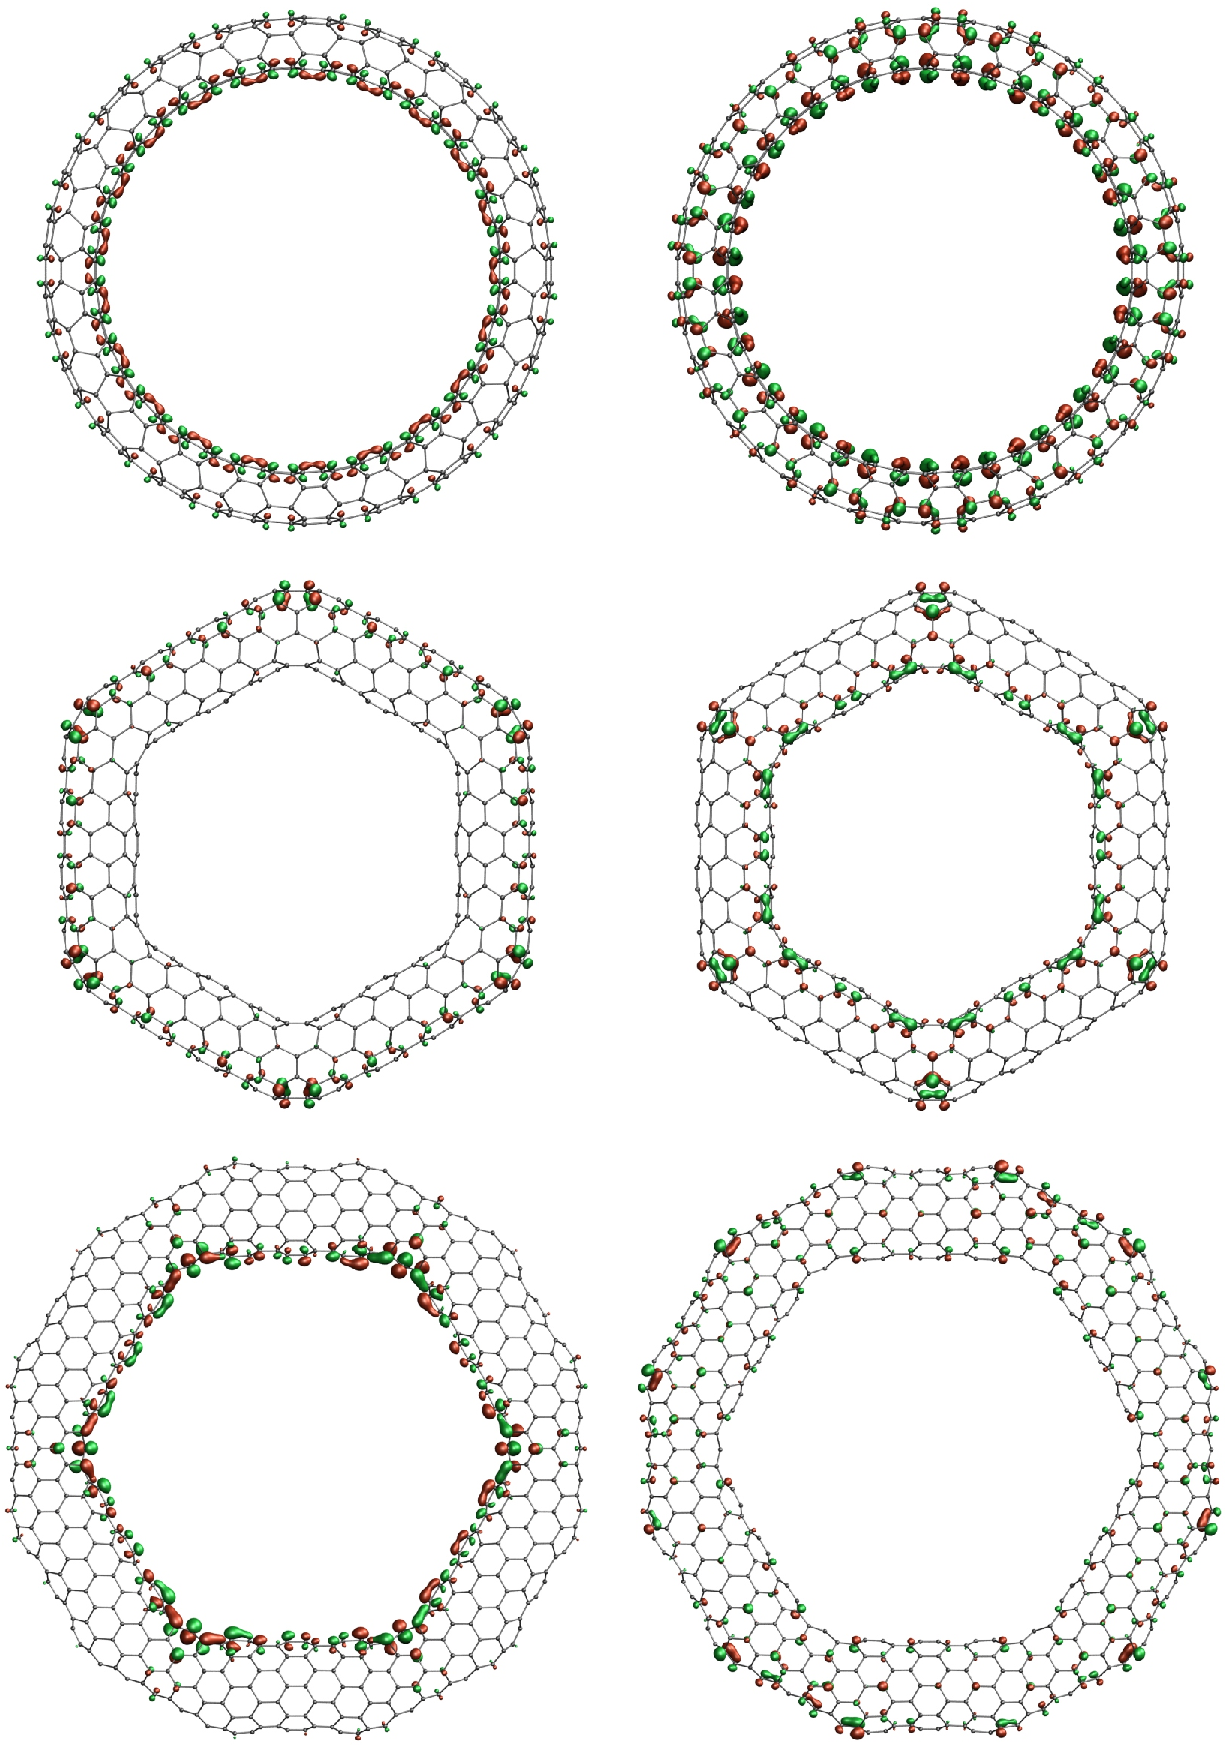
\includegraphics[width=0.92\textwidth]{homolumozigzag}
	\captionsetup{figurewithin = chapter}
	\captionsetup{font=small, labelfont=bf}\caption[HOMO und LUMO von toroidalen Kohlenstoff-Nanoröhren 2]{HOMOs (links) und LUMOs (rechts) von toroidalen Kohlenstoff-Nanoröhren (\acp{tcnt}). C$_{588}$: \textit{polyhex}-\textit{zigzag}-\ac{tcnt} (7,0),($-$21,42) (oben), C$_{588}$: Chuang-\textit{zigzag}-\ac{tcnt} (1,2,2,3),(1,1) (Mitte) und C$_{864}$: Dunlap-\textit{armchair-zigzag}-\ac{tcnt} 2(4,4),3(8,0) (unten). Die Konturen von HOMO und LUMO wurden bei \unit[0.018]{a.u.} (grün) und \unit[$-$0.018]{a.u.} (rot) gezeichnet.}
\label{abb:homolumozigzag}
\end{figure}

\FloatBarrier
\subsection{Zusammenfassung}
Zusammenfassend zeigen die Untersuchungen unterschiedlicher \ac{tcnt}-Strukturtypen, dass große Ringströme in diesen Systemen auftreten können. Das Auftreten hängt jedoch stark von den strukturellen Parametern und der damit einhergehenden elektronischen Struktur der jeweiligen Verbindung ab. Tendenziell wird insbesondere in \textit{polyhex}-\acp{tcnt} ein großer Ringstrom erhalten, was für eine starke Delokalisierung der Elektronen darin spricht. Dies steht in guter Übereinstimmung mit dem metallischen Charakter dieser Strukturen. Eine Untersuchung des Einflusses der Ringgröße auf den Strom konnte dabei zeigen, dass letztgenannter mit zunehmender Systemgröße der \ac{tcnt} steigt. Auch \acp{tcnt} mit fünf- und siebengliedrigen Ringen können große Ringströme aufweisen. Diese fallen in der Regel jedoch etwas kleiner als bei den entsprechenden \textit{polyhex}-Strukturen aus, und sind stark abhängig von der Lage und Orientierung der pentagonalen und heptagonalen Einheiten. Notwendig für das Auftreten von Ringströmen ist zudem ein möglichst kleines HOMO-LUMO-Gap, welches alleine jedoch noch keine hinreichende Bedingung darstellt.

\section{Anwendungen in der anorganischen Chemie}
\FloatBarrier
\subsection{\texorpdfstring{$[$Hg$_8$Te$_8$(Te$_2$)$_4$]$^{8-}$}{[Hg\_8Te\_8(Te\_2)\_4]8-}: Ein anorganisches Porphyrin?}\label{anorgporh}
Die Implementierung des \ac{cosmo}\supercite{klamt1993cosmo} und der \acp{ecp} in das \texttt{mpshift}-Modul liefert die notwendigen Voraussetzungen, um einen tieferen Einblick in magnetische Eigenschaften anionischer Verbindungen, welche schwere Elemente beinhalten, zu erhalten. Ein Beispiel dafür ist das in der Arbeitsgruppe von Stephanie Dehnen synthetisierte $[$Hg$_8$Te$_8$(Te$_2$)$_4$]$^{8-}$\supercite{dehnenhg4te8}, welches auf der linken Seite in Abbildung \ref{abb:hg8te16undb8s16} gezeigt ist. Die Seitenansicht zeigt das Molekül mit TPSSh\supercite{tao2003climbing}/def2-TZVP\supercite{weigend2005balanced} optimierten Strukturparametern. Zusätzlich wurden die entsprechenden Auxiliarbasisfunktionen\supercite{weigend2006accurate} und \acp{ecp}\supercite{peterson2003systematically} verwendet. Die Kompensation der Ladung erfolgte durch das \ac{cosmo}. In der Abbildung ist zu erkennen, dass das Anion nicht vollständig planar ist und damit auch leicht von der idealen $D_{4\textrm{h}}$ symmetrischen Struktur abweicht. 
\begin{figure}[ht!]
	\centering
	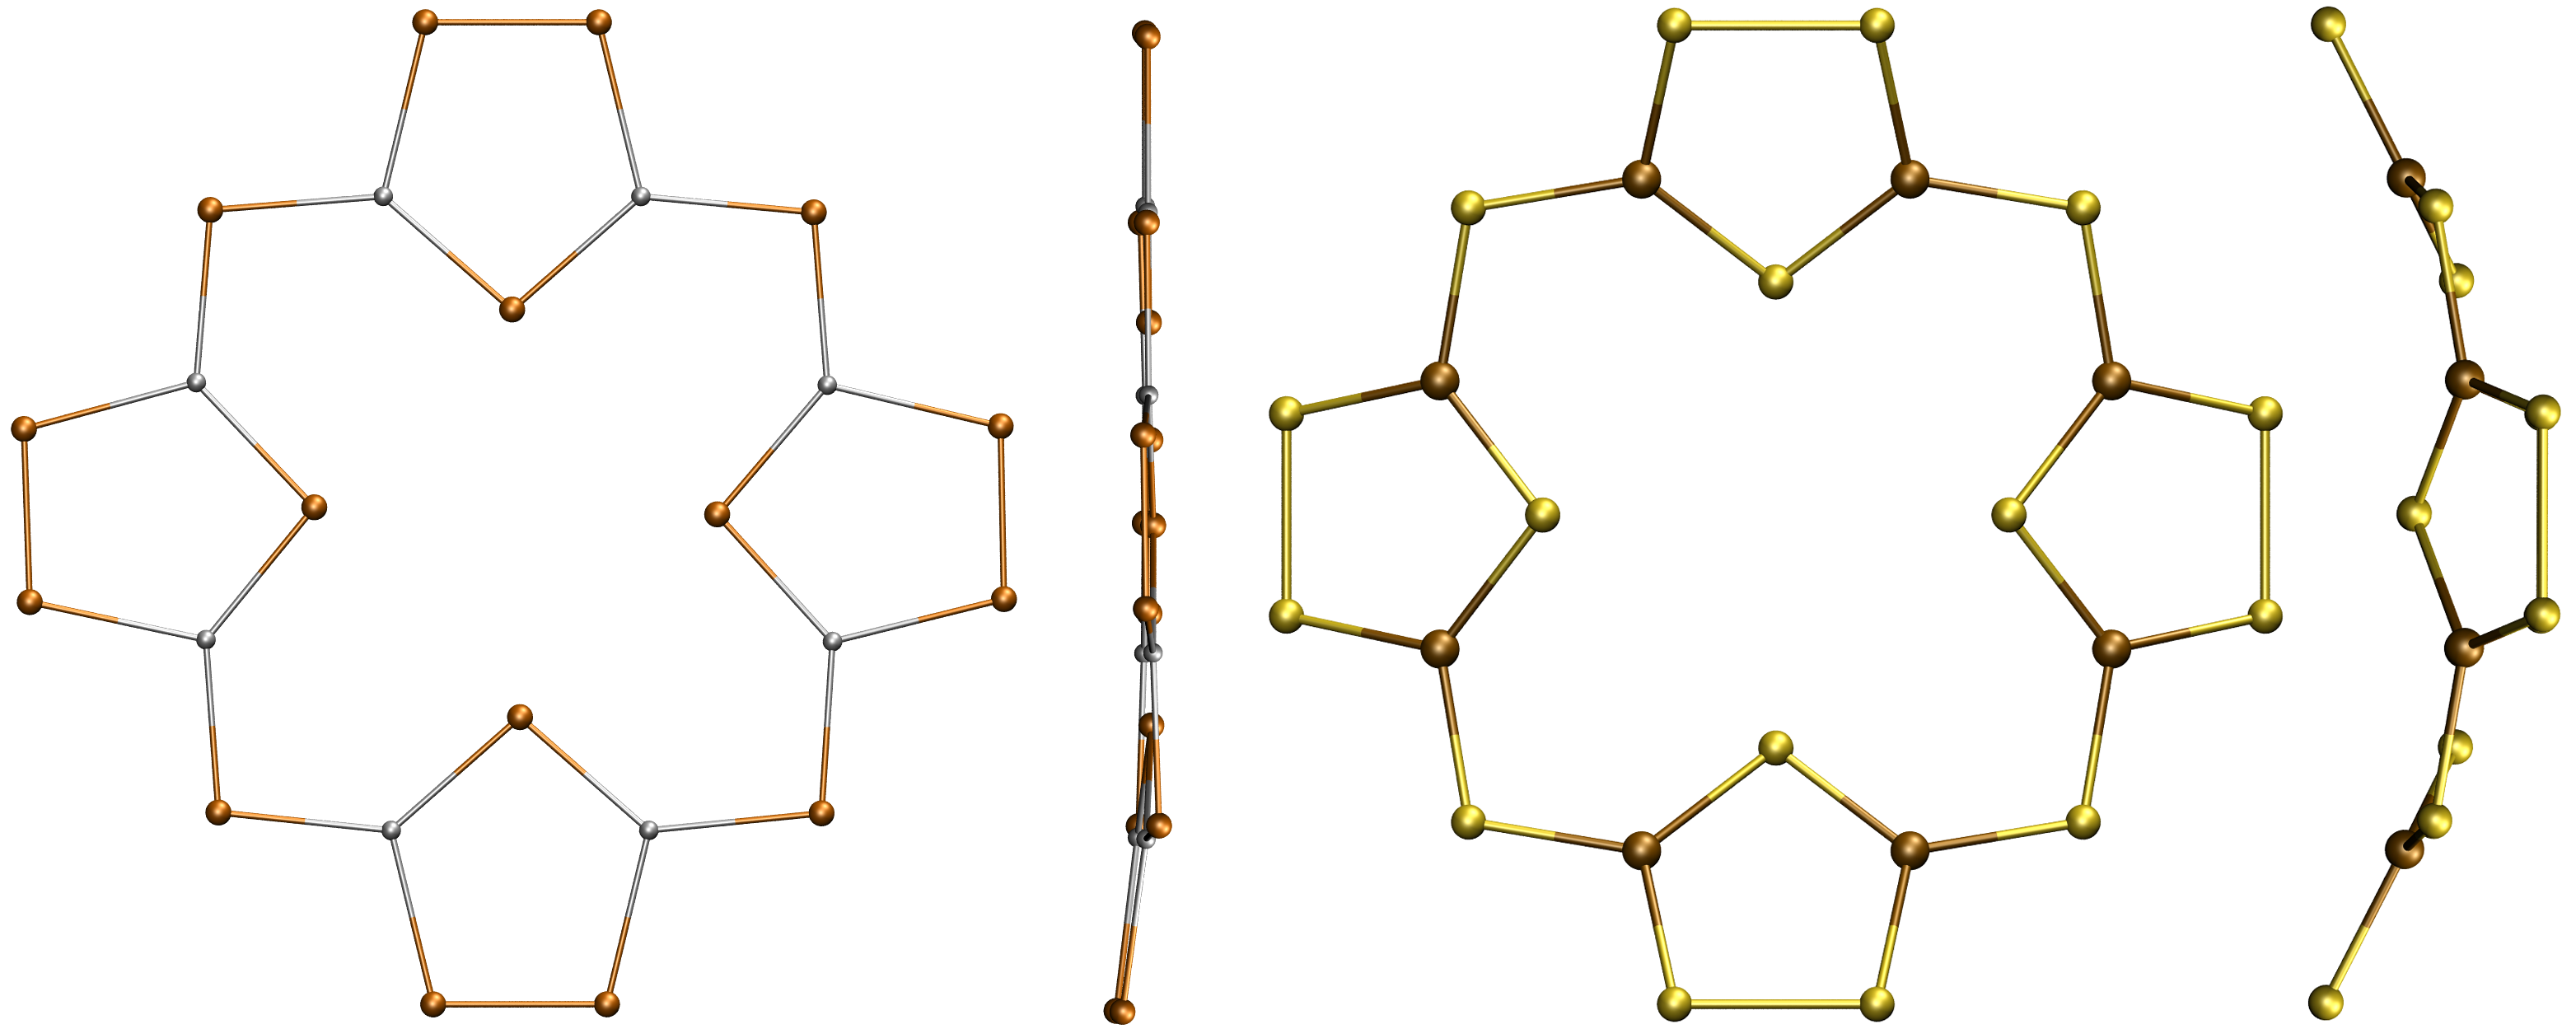
\includegraphics[width=1.0\textwidth]{hg8te16undb8s16}
	\captionsetup{figurewithin = chapter}
	\captionsetup{font=small, labelfont=bf}\caption[{Abbildung von $[$Hg$_8$Te$_8$(Te$_2$)$_4$]$^{8-}$ und B$_8$S$_8$(S$_2$)$_4$}]{Draufsicht und Seitenansicht von $[$Hg$_8$Te$_8$(Te$_2$)$_4$]$^{8-}$ (links) und B$_8$S$_8$(S$_2$)$_4$ (rechts) (Quecksilber=silber, Tellur=orangebraun, Bor=braun und Schwefel=gelb).}
\label{abb:hg8te16undb8s16}
\end{figure}
%\begin{figure}[ht!]
%	\centering
%	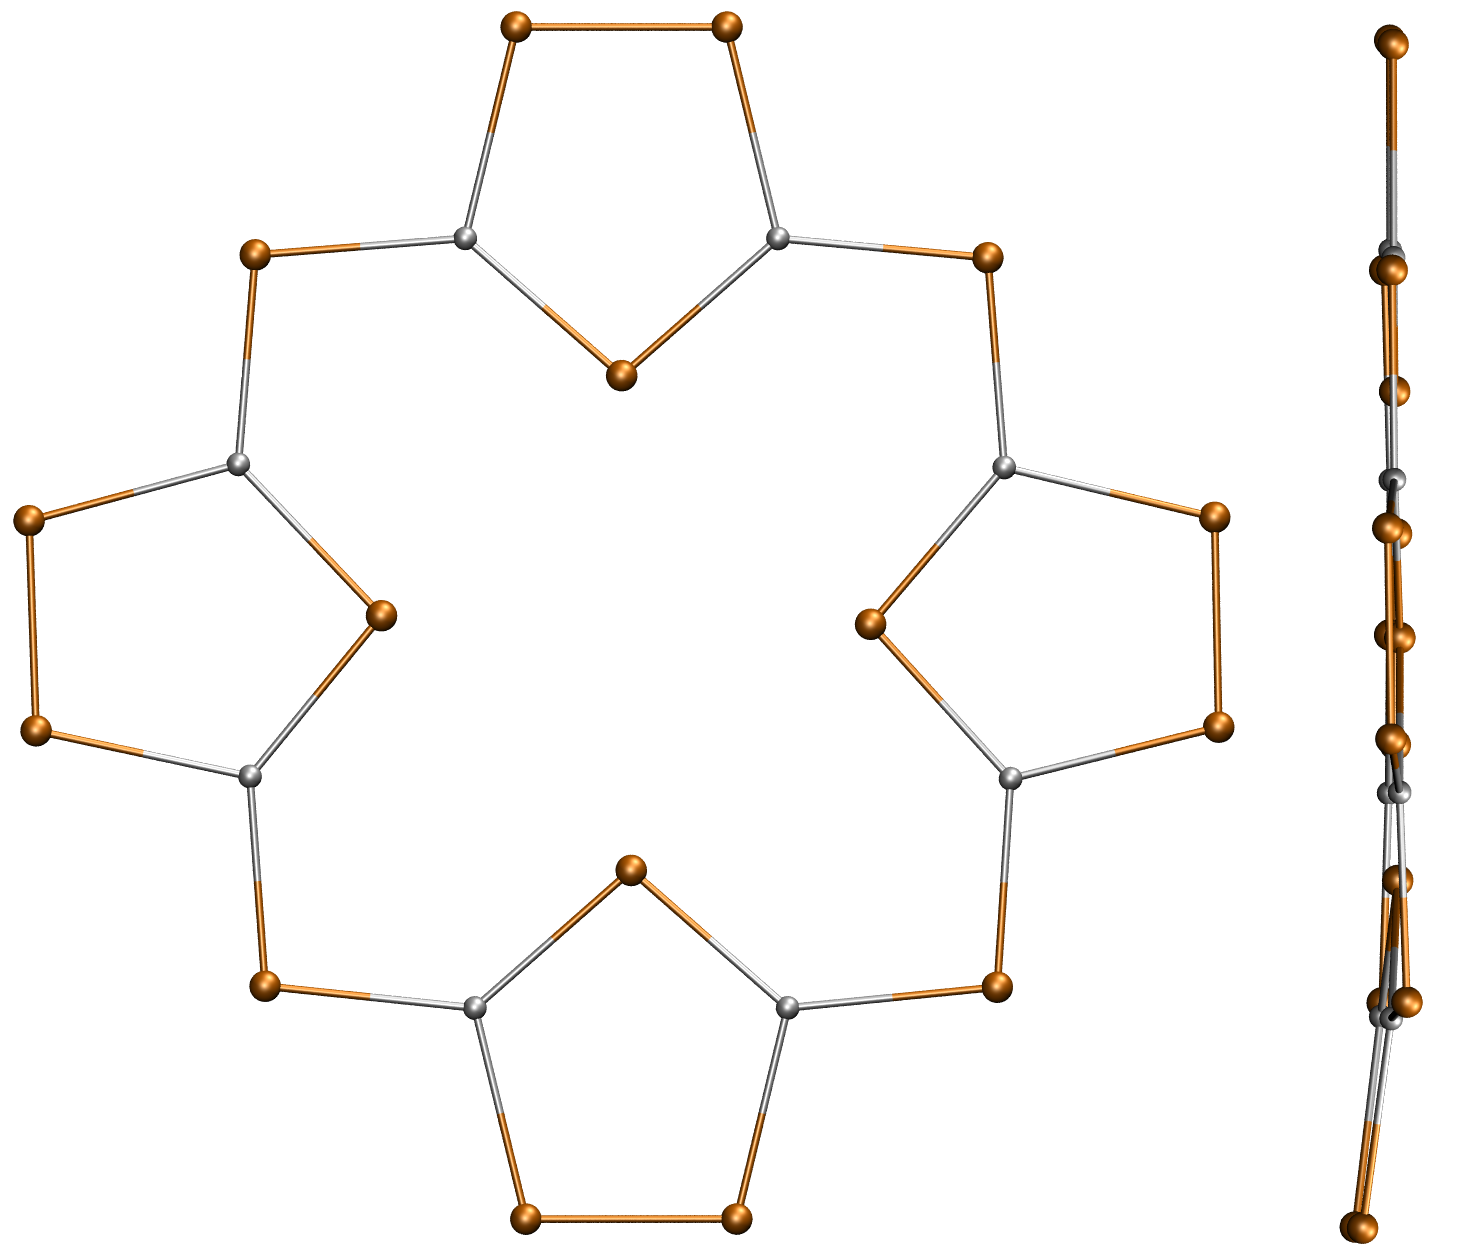
\includegraphics[width=0.6\textwidth]{hg8te16}
%	\captionsetup{figurewithin = chapter}
%	\captionsetup{font=small, labelfont=bf}\caption[{Abbildung von $[$Hg$_8$Te$_{16}]^{8-}$}]{{Abbildung von $[$Hg$_8$Te$_{16}]^{8-}$}(Quecksilber=silber, Tellur=orangebraun). Draufsicht links und Seitenansicht rechts.}
%\label{abb:hg8te16}
%\end{figure}

Zusätzlich wurde ebenfalls das bereits bekannte B$_8$S$_8$(S$_2$)$_4$\supercite{krebs1980b8s16} (Abbildung \ref{abb:hg8te16undb8s16} rechts) untersucht. Hier ist die Abweichung des Moleküls mit optimierten Strukturparametern von der planaren Struktur erheblich größer, wie die Seitenansicht deutlich zeigt. Die $D_{4\textrm{h}}$ symmetrische Struktur weist eine schwache imaginäre Mode von etwa \unit[$-$10]{cm$^{-1}$} auf, welche genau der Gerüstschwingung entspricht, die das Durchschwingen des Moleküls beschreibt. Ebenfalls bekannt ist das schwerere Homolog B$_8$Se$_8$(Se$_2$)$_4$.
%\begin{figure}[ht!]
%	\centering
%	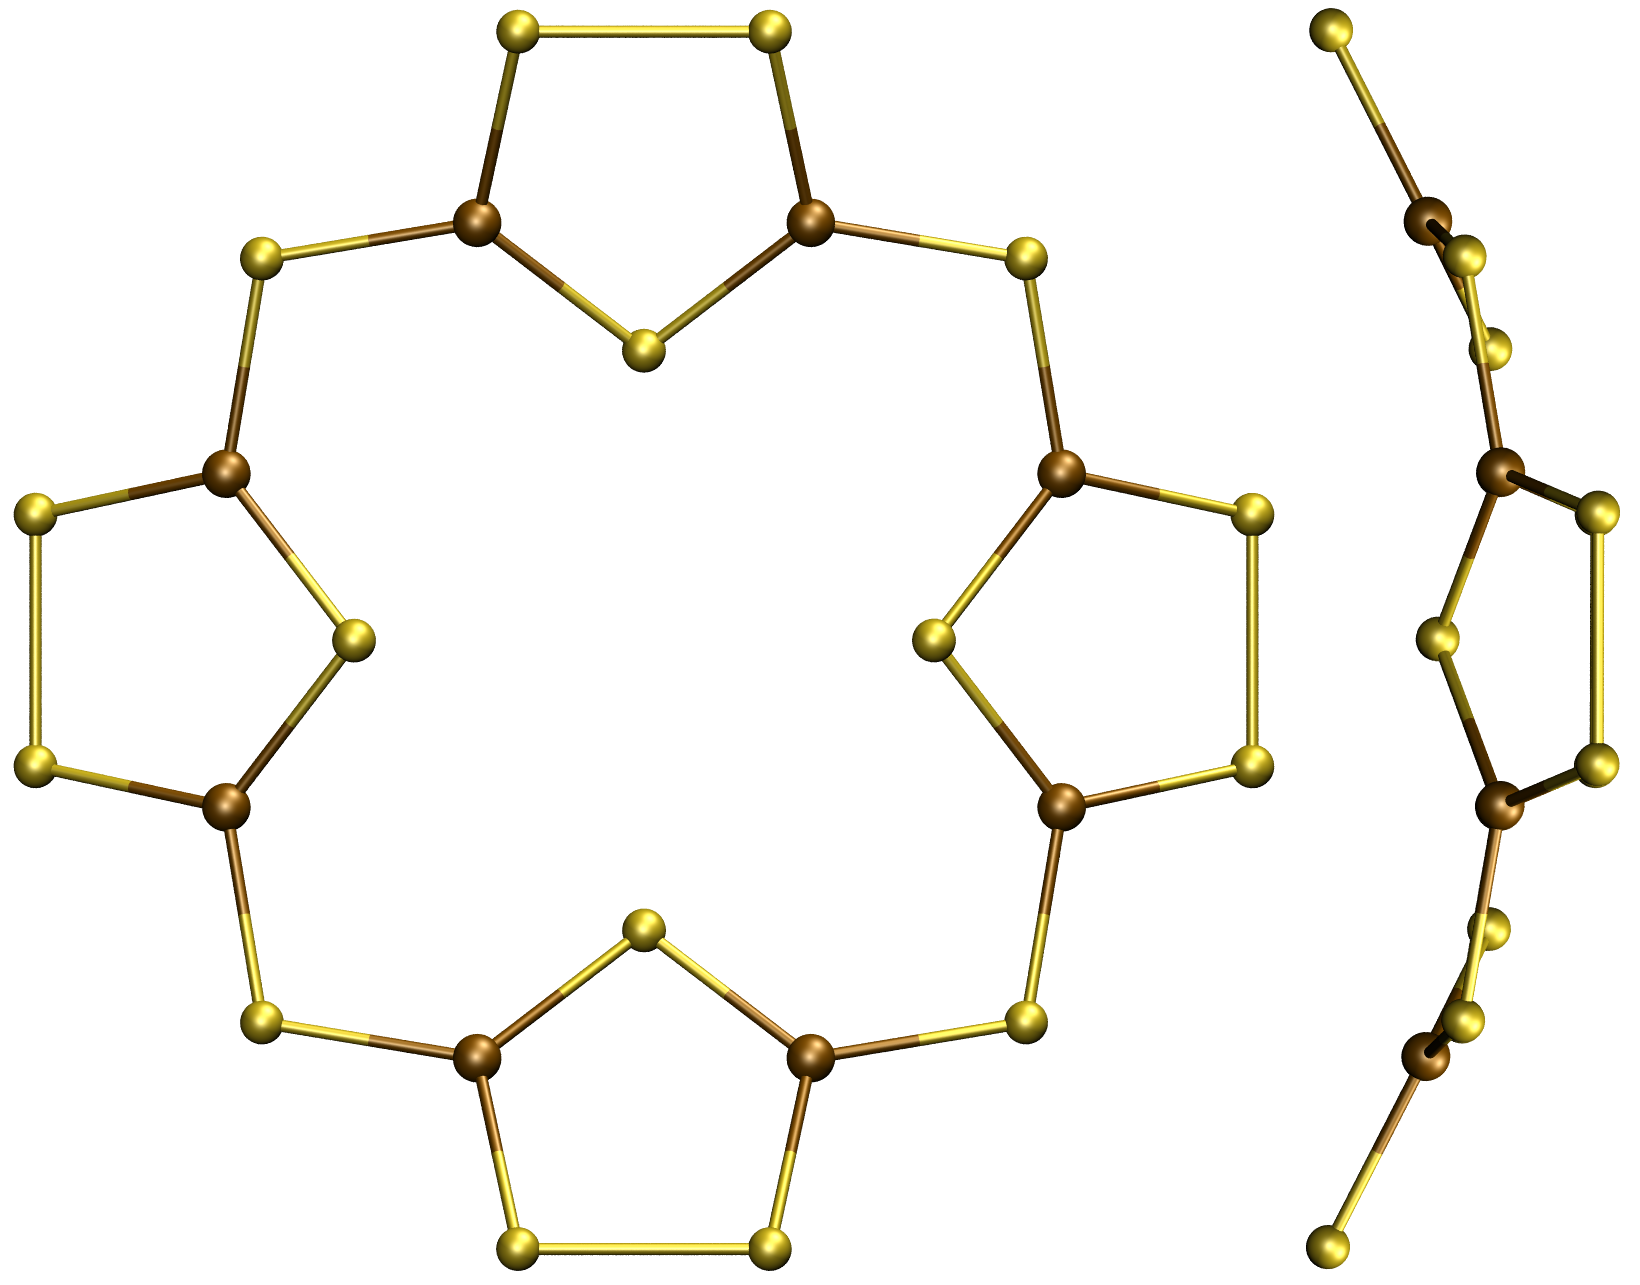
\includegraphics[width=0.6\textwidth]{b8s16}
%	\captionsetup{figurewithin = chapter}
%	\captionsetup{font=small, labelfont=bf}\caption[Abbildung von B$_8$S$_{16}$]{Abbildung von B$_8$S$_{16}$(Bohr=braun, Schwefel=gelb). Draufsicht links und Seitenansicht rechts.}
%\label{abb:b8s16}
%\end{figure}

Aufgrund ihrer strukturellen Ähnlichkeit mit dem organischen Porphyrin liegt es nahe, den aromatischen Charakter der Verbindungen zu untersuchen. Als Maß für die Aromatizität der Verbindung kann auch hier die Stärke des Gesamtringstroms herangezogen werden. Je diatropischer der Gesamtringstrom ist, desto aromatischer ist die Verbindung. In den oben erwähnten Beispielen kann weiterhin zwischen einem lokalen Ringstrom in den vier Fünfringen und einem globalen Ringstrom um das gesamte Molekül unterschieden werden. Hierfür erfolgt die numerische Integration des Stromes durch eine Ebene, welch senkrecht zu ausgewählten Bindungen platziert wird. Auf diese weise lässt sich der Pfad des Ringstromes verfolgen. Bei den Berechnungen stellte sich heraus, dass alle drei Verbindungen, $[$Hg$_8$Te$_8$(Te$_2$)$_4$]$^{8-}$, B$_8$S$_8$(S$_2$)$_4$ und B$_8$Se$_{16}$, einen schwachen lokalen Ringstrom in den pyrrolartigen fünfgliedrigen Ringen aufweisen. Diese betragen \unit[5.8]{nA/T} in $[$Hg$_8$Te$_8$(Te$_2$)$_4$]$^{8-}$, \unit[3.25]{nA/T} in B$_8$S$_8$(S$_2$)$_4$ und \unit[3.28]{nA/T} in B$_8$Se$_8$(Se$_2$)$_4$. Im Vergleich dazu beträgt der Ringstrom in einem Benzolmolekül etwa \unit[12]{nA/T}\supercite{fliegl2012aromatic}. Die globalen Ringströme in den drei Verbindungen sind mit \unit[0.24]{nA/T}, \unit[0.81]{nA/T} und \unit[0.79]{nA/T} verschwindend gering. Im Vergleich dazu liegt der globale Ringstrom des organischen Porphyrins bei etwa \unit[27]{nA/T}. Dieser spaltet sich in den fünfgliedrigen Ringen in einen äußeren und inneren Pfad auf, welche jeweils einen Ringstrom von etwa \unit[13]{nA/T} aufweisen. Der lokale Ringstrom in den fünfgliedrigen Ringen ist schwächer als \unit[1]{nA/T}.\supercite{fliegl2012aromatic} In sogenannten \aclu*{lic-}\mbox{(\acs{lic}-)}\acused{lic}Plots lassen sich die Ringströme in einer gewählten Ebene visualisieren. Eine solche Darstellung des Ringstroms ist für das organische Porphyrin und die drei Verbindungen $[$Hg$_8$Te$_8$(Te$_2$)$_4$]$^{8-}$, B$_8$S$_8$(S$_2$)$_4$ und B$_8$Se$_8$(Se$_2$)$_4$ in der Abbildung \ref{abb:lic} zu sehen. Beim Porphyrin ist eindeutig der globale Ringstrom zu erkennen, welcher sich in den fünfgliedrigen Ringen in zwei Pfade aufspaltet. Im Vergleich dazu weisen die anderen Verbindungen lediglich schwache lokale Ströme in den fünfgliedrigen Ringen auf.
Diese Befunde lassen sich dadurch erklären, dass im Porphyrin eine völlig andere elektronische Situation vorliegt. Die Aromatizität und die damit verbundenen Ringströme basieren auf einem delokalisierten $\pi$-System. Beispielsweise lassen sich im $[$Hg$_8$Te$_8$(Te$_2$)$_4$]$^{8-}$ alle \acp{mo} durch Anwenden einer Lokalisierungsprozedur\supercite{boys1960sf} zu Zweizentren-Zweielektronen-Bindungen und freien Elektronenpaaren lokalisieren. Dabei werden $\sigma$-artige Einfachbindungen zwischen den benachbarten Atomen und zwei freie Elektronenpaare pro Telluratom erhalten. 

 

\begin{figure}[ht!]
	\centering
	\includegraphics[width=1.0\textwidth]{1bohr}
	\captionsetup{figurewithin = chapter}
	\captionsetup{font=small, labelfont=bf}\caption[{Porphyrin, $[$Hg$_8$Te$_8$(Te$_2$)$_4$]$^{8-}$, B$_8$S$_8$(S$_2$)$_4$ und B$_8$Se$_8$(Se$_2$)$_4$: \aclu{lic-}Plots der Ringströme}]{\aclu{lic-}Plots der Ringströme in Porphyrin \textsf{(a)}, $[$Hg$_8$Te$_8$(Te$_2$)$_4$]$^{8-}$ \textsf{(b)}, B$_8$S$_8$(S$_2$)$_4$ \textsf{(c)} und B$_8$Se$_8$(Se$_2$)$_4$ \textsf{(d)} \unit[1]{$a_0$} oberhalb der Molekülebene, dargestellt zwischen \unit[0]{a.\,u.} (blau) und \unit[0.07]{a.\,u.}}
\label{abb:lic}
\end{figure}

\FloatBarrier
Das fehlende $\pi$-System im $[$Hg$_8$Te$_8$(Te$_2$)$_4$]$^{8-}$ sorgt für eine gewisse strukturelle Flexibilität des Makrozyklus. Dadurch können unterschiedliche Koordinationspolyeder und Koordinationszahlen realisiert werden. Die Strukturparameter wurden exemplarisch für die Komplexierung der Metallkationen Zn$^{2+}$, Cu$^+$, Ce$^{4+}$ und Ti$^{4+}$ optimiert und die erhaltenen Strukturen sind in Abbildung \ref{abb:komplexierung} gezeigt. Für Zn$^{2+}$ und Cu$^+$ ist zu erkennen, dass es dabei im Wesentlichen zu einer Verzerrung des Makrozyklus kommt um eine tetraedrische Koordination zu ermöglichen. Im Falle der Ce$^{4+}$- und Ti$^{4+}$-Kationen führt die Komplexierung zu einer deutlich ausgeprägteren Umordnung der Atome. Damit lassen sich sowohl die bevorzugt größere Koordinationszahl des Ce$^{4+}$ als auch die Anpassung an den deutlich geringeren Ionenradius des Ti$^{4+}$ realisieren.

\begin{figure}[ht!]
	\centering
	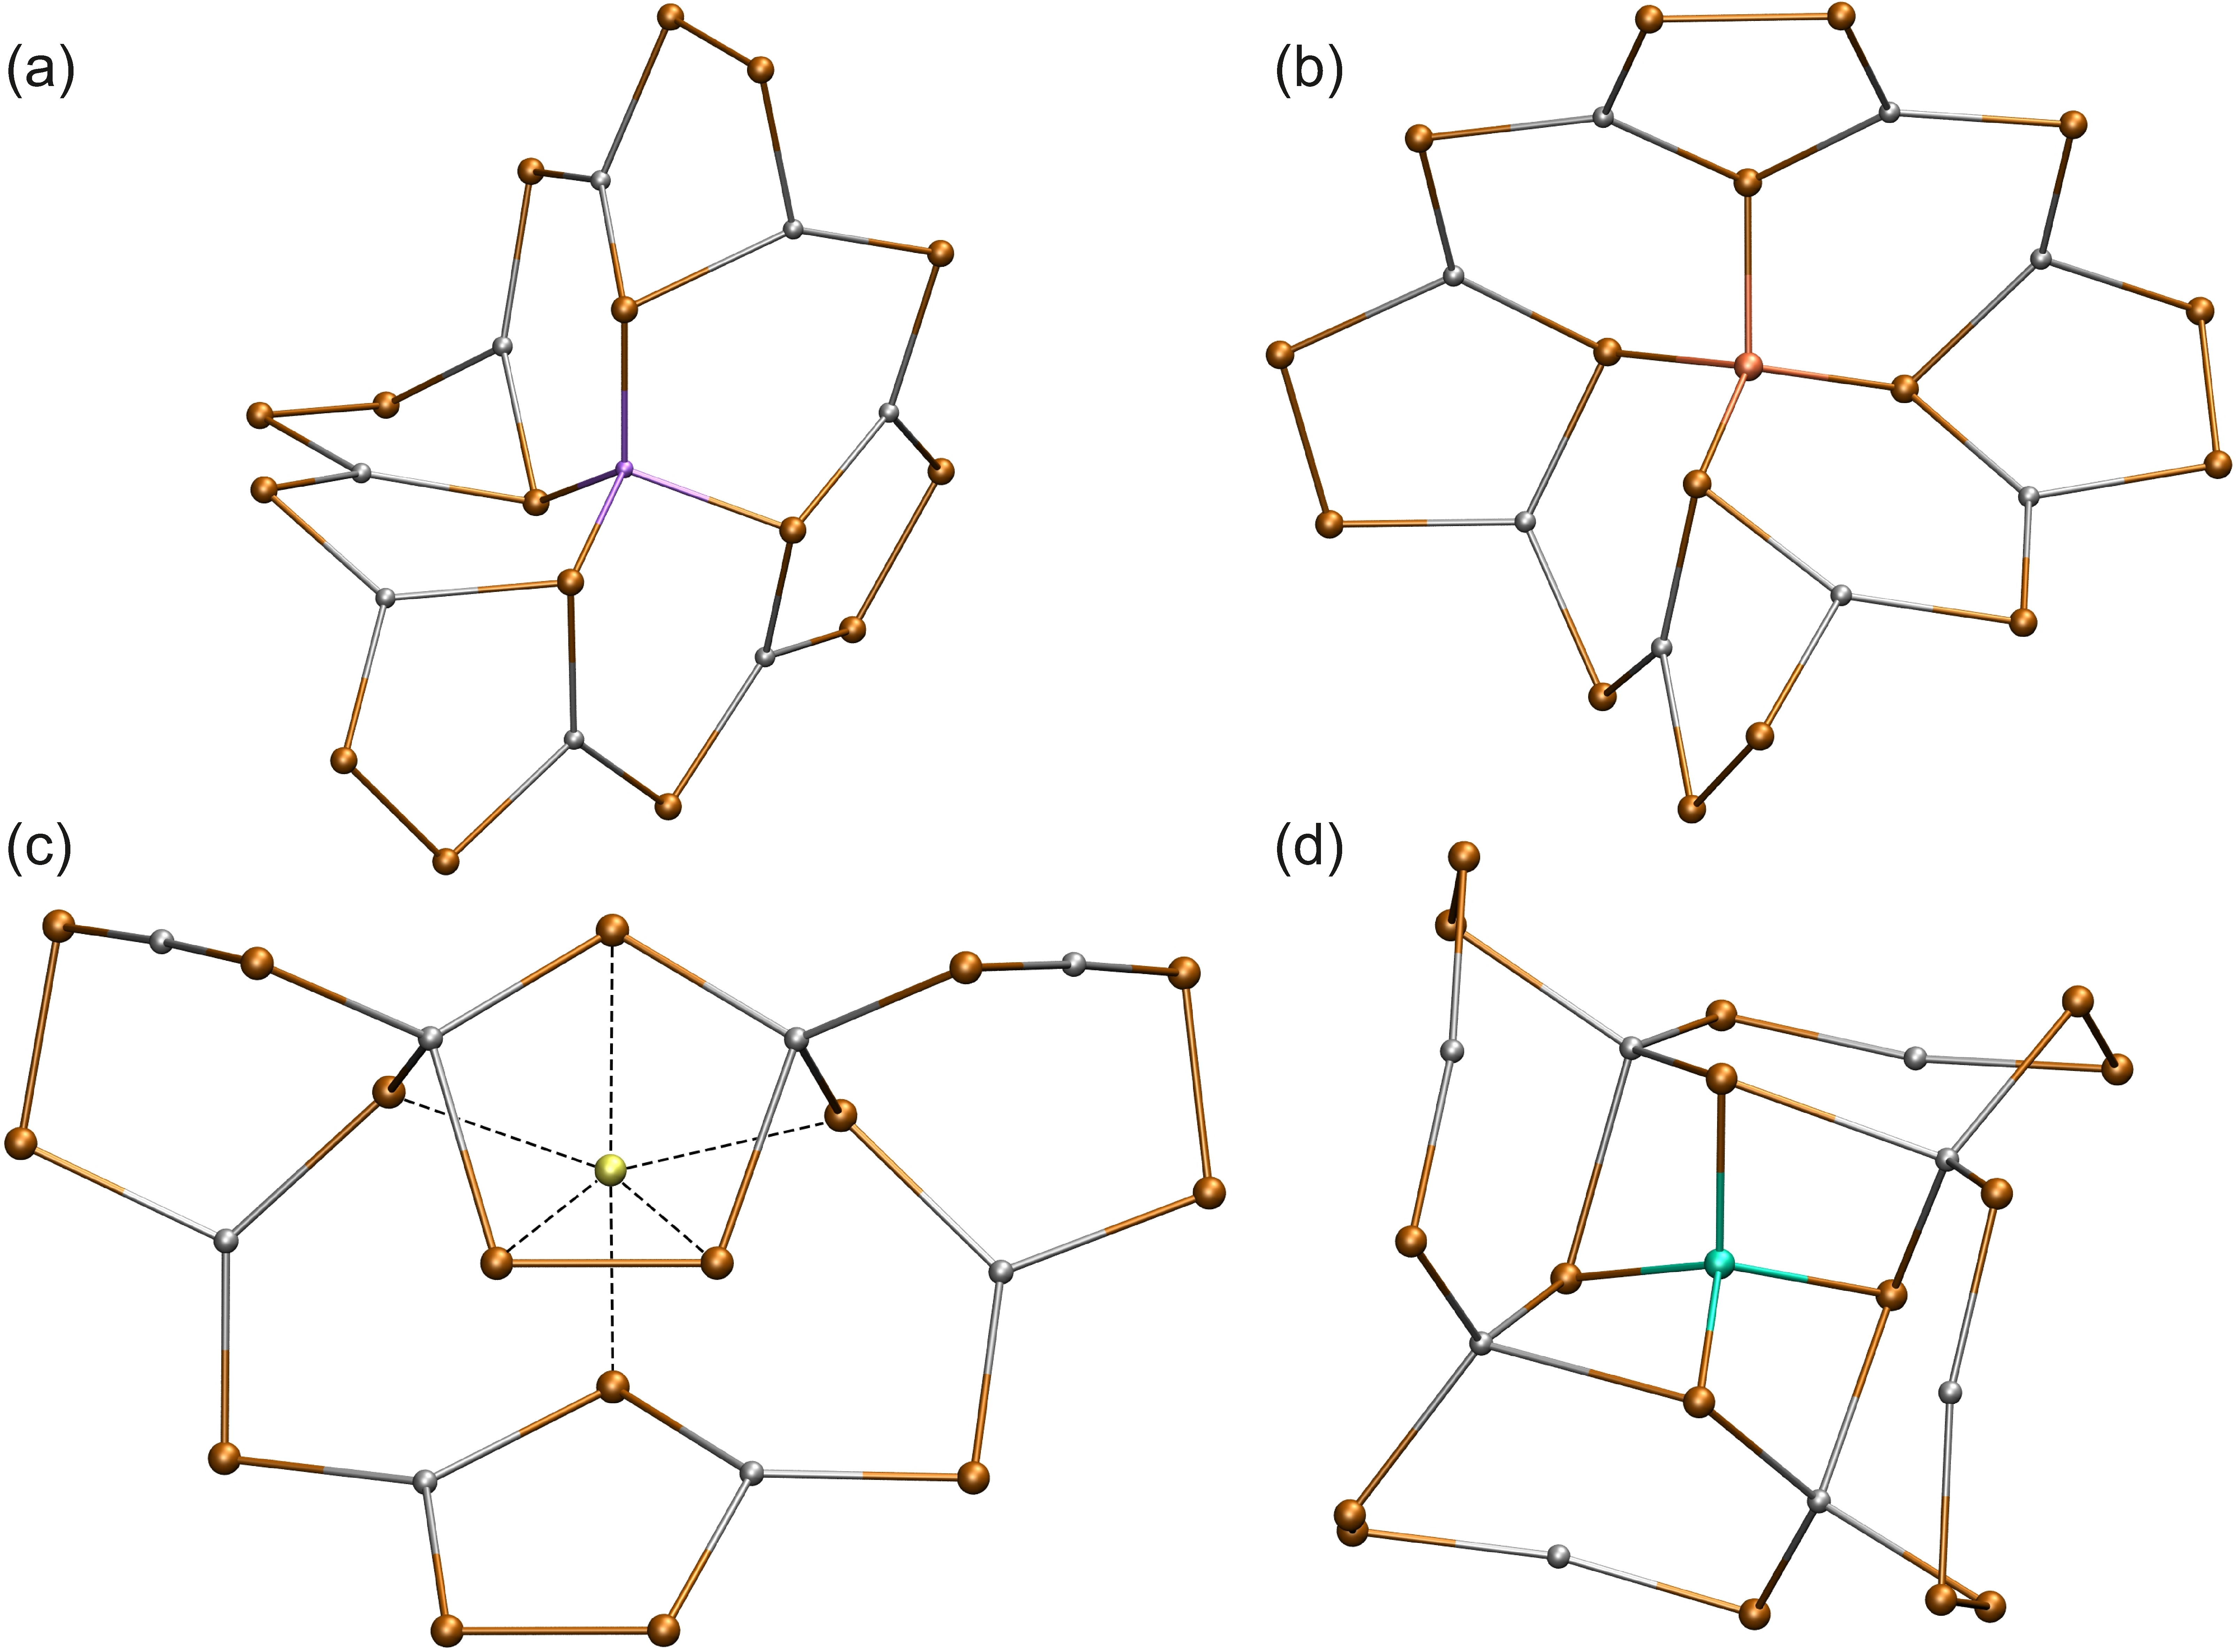
\includegraphics[width=1.0\textwidth]{komplexierung}
	\captionsetup{figurewithin = chapter}
	\captionsetup{font=small, labelfont=bf}\caption[{Abbildungen der hypothetischen Komplexe [M@Hg$_8$Te$_8$(Te$_2$)$_4]^{(8-q)-}$ (M$^{q+}$ = Zn$^{2+}$, Cu$^+$ , Ce$^{4+}$ und Ti$^{4+}$)}]{{Abbildung der hypothetischen Komplexe [M@Hg$_8$Te$_8$(Te$_2$)$_4]^{(8-q)-}$ (M$^{q+}$ = Zn$^{2+}$ \textsf{(a)}, Cu$^+$ \textsf{(b)}, Ce$^{4+}$ \textsf{(c)} und Ti$^{4+}$ \textsf{(d)})} zur Veranschaulichung der strukturellen Flexibilität von $[$Hg$_8$Te$_8$(Te$_2$)$_4$]$^{8-}$ (Quecksilber=silber, Tellur=orangebraun, Zink=lilablau, Kupfer=kupfer, Cer=hellgelb, Titan=türkis). }
\label{abb:komplexierung}
\end{figure}

%\begin{figure}[ht!]
%	\centering
%	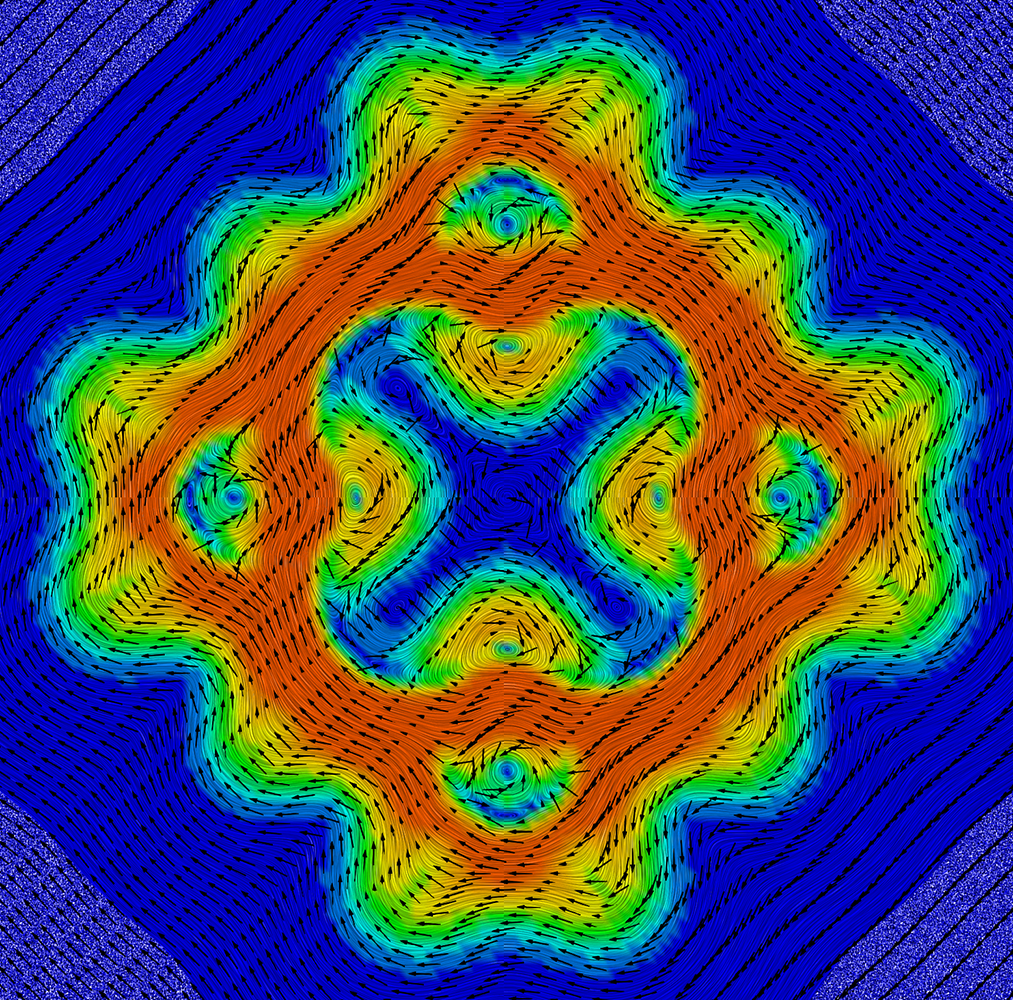
\includegraphics[width=0.6\textwidth]{porph_1bohr}
%	\captionsetup{figurewithin = chapter}
%	\captionsetup{font=small, labelfont=bf}\caption[Ringströme in Porphyrin]{Ringströme in Porphyrin \unit[1]{bohr} oberhalb der Molekülebene, dargestellt zwischen \unit[0]{a.u.} (blau) und \unit[0.07]{a.u.}.}
%\label{abb:porphlic}
%\end{figure}
%
%\begin{figure}[ht!]
%	\centering
%	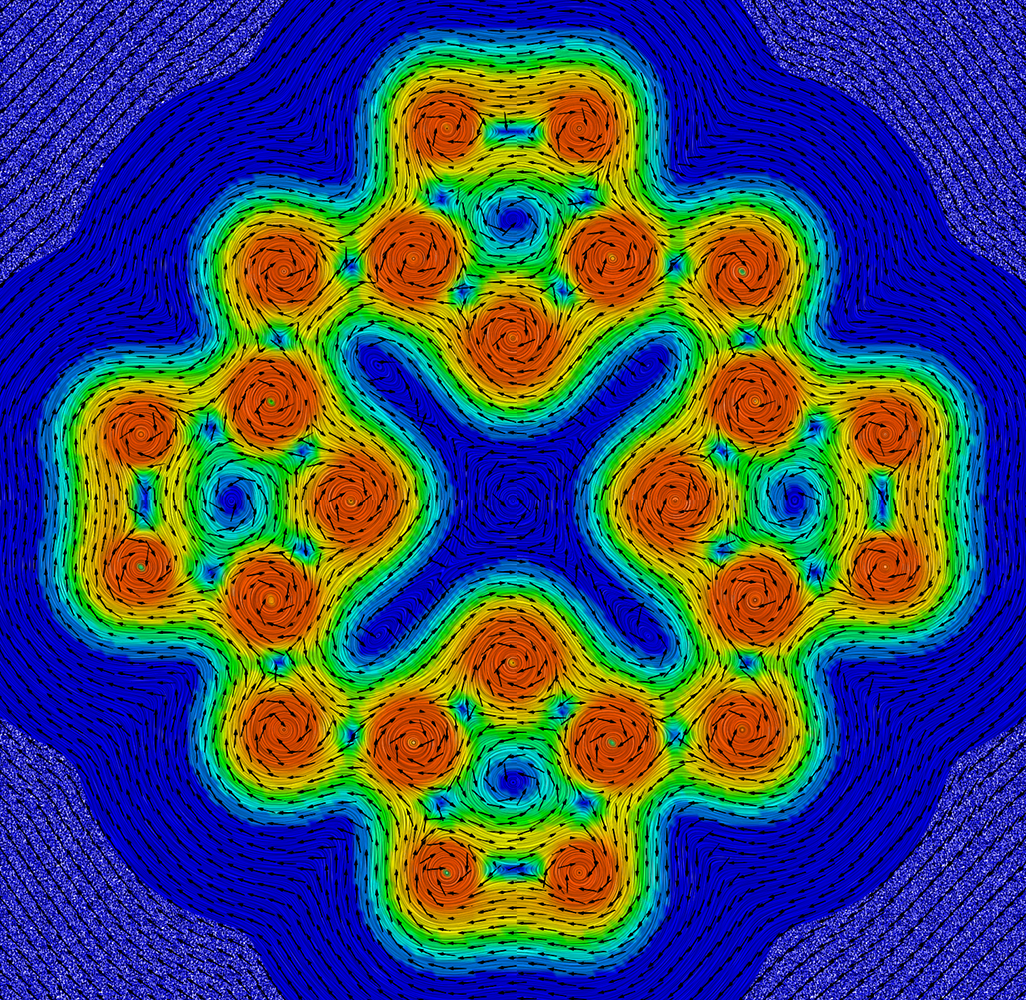
\includegraphics[width=0.6\textwidth]{hgte_1bohr}
%	\captionsetup{figurewithin = chapter}
%	\captionsetup{font=small, labelfont=bf}\caption[{Ringströme in $[$Hg$_8$Te$_8$(Te$_2$)$_4]^{8-}$}]{Ringströme in $[$Hg$_8$Te$_8$(Te$_2$)$_4]^{8-}$ \unit[1]{bohr} oberhalb der Molekülebene, dargestellt zwischen \unit[0]{a.u.} (blau) und \unit[0.07]{a.u.}.}
%\label{abb:hgtelic}
%\end{figure}
%
%\begin{figure}[ht!]
%	\centering
%	\includegraphics[width=0.6\textwidth]{b8s16_1bohr}
%	\captionsetup{figurewithin = chapter}
%	\captionsetup{font=small, labelfont=bf}\caption[Ringströme in B$_8$S$_{16}$]{Ringströme in B$_8$S$_{16}$ \unit[1]{bohr} oberhalb der Molekülebene, dargestellt zwischen \unit[0]{a.u.} (blau) und \unit[0.07]{a.u.}.}
%\label{abb:b8s16hlic}
%\end{figure}
%
%\begin{figure}[ht!]
%	\centering
%	\includegraphics[width=0.6\textwidth]{b8se16_1bohr}
%	\captionsetup{figurewithin = chapter}
%	\captionsetup{font=small, labelfont=bf}\caption[Ringströme in B$_8$Se$_{16}$]{Ringströme in B$_8$Se$_{16}$ \unit[1]{bohr} oberhalb der Molekülebene, dargestellt zwischen \unit[0]{a.u.} (blau) und \unit[0.07]{a.u.}.}
%\label{abb:b8se16hlic}
%\end{figure}
\FloatBarrier
\subsection{\texorpdfstring{$^{119}$Sn-\acs{nmr}-Spektren von [Co@Sn$_6$Sb$_6$]$^{3-}$ und [Co$_2$@Sn$_5$Sb$_7$]$^{3-}$}{119Sn-NMR Spektren von [Co at Sn\_6Sb\_6]3- und [Co\_2 at Sn\_5Sb\_7]3-}}
Wie bereits in der Einleitung dieser Arbeit erwähnt wird, kann die Zuordnung einzelner Signale in experimentell gemessenen \ac{nmr}-Spektren in manchen Fällen eine große Herausforderung darstellen. Zwei Beispiele dafür sind die $^{119}$Sn-\ac{nmr}-Spektren der in der Arbeitsgruppe von Stefanie Dehnen synthetisierten Clusteranionen [Co@Sn$_6$Sb$_6$]$^{3-}$ und [Co$_2$@Sn$_5$Sb$_7$]$^{3-}$.\supercite{wilson2018structure} Die grundlegende Struktur dieser endohedralen Komplexe besteht aus zwei verbundenen quadratischen Antiprismen und ist in Abbildung \ref{abb:coatsnsb} dargestellt. Interessanterweise befindet sich das Cobaltatom im Falle des [Co@Sn$_6$Sb$_6$]$^{3-}$ nicht im Zentrum des gesamten Clusteranions, sondern im Zentrum eines der quadratischen Antiprismen. Mithilfe eines genetischen Algorithmus\supercite{weigend2014extending} konnten diese ungewöhnlichen Strukturen auf \ac{dft}-Niveau bestätigt werden. Die Zuordnung der Atomsorten erfolgt darin über einen störungstheoretischen Ansatz. Für den genetischen Algorithmus wurde das BP86-Funktional\supercite{perdew1986density,becke1988density} und der Basissatz def-SV(P)\supercite{eichkorn1997auxiliary} verwendet. Die Anzahl der Generationen wurde auf 30 und die Anzahl der Strukturen je Generationen auf 25 festgelegt. In jeder Generation wurden die 13 energetisch ungünstigsten Strukturen durch neu generierte ersetzt. Alle 25 Strukturen der letzten Generation weisen das Grundgerüst von zwei verknüpften quadratischen Antiprismen auf, welches für die energetisch höher liegenden Isomere jedoch stärker verzerrt ist. Die Strukturparameter der Clusteranionen aus der letzten Generation wurden  mit dem TPSS-Funktional\supercite{tao2003climbing} und der Basis dhf-TZVP\supercite{weigend2010segmented} sowie den zugehörigen \acp{ecp}\supercite{metz2000small} für Zinn und Antimon nachoptimiert. Die negative Ladung wurde mithilfe des \ac{cosmo}\supercite{klamt1993cosmo} unter Verwendung der Standardeinstellungen kompensiert. Insgesamt unterscheiden sich die Strukturen im Wesentlichen durch die Verteilung der Atomsorten und liegen in einem Energiebereich von \unit[37]{kJ/mol} ([Co@Sn$_6$Sb$_6$]$^{3-}$) und \unit[22]{kJ/mol} ([Co$_2$@Sn$_5$Sb$_7$]$^{3-}$). Für die erste Verbindung wurden zwei nahezu isoenergetische Isomere gefunden (linke Seite und Mitte von Abbildung \ref{abb:coatsnsb}). Die energetisch günstigste Struktur des zweiten Clusteranions ist auf der rechten Seite der Abbildung gezeigt.

\begin{figure}[ht!]
	\centering
	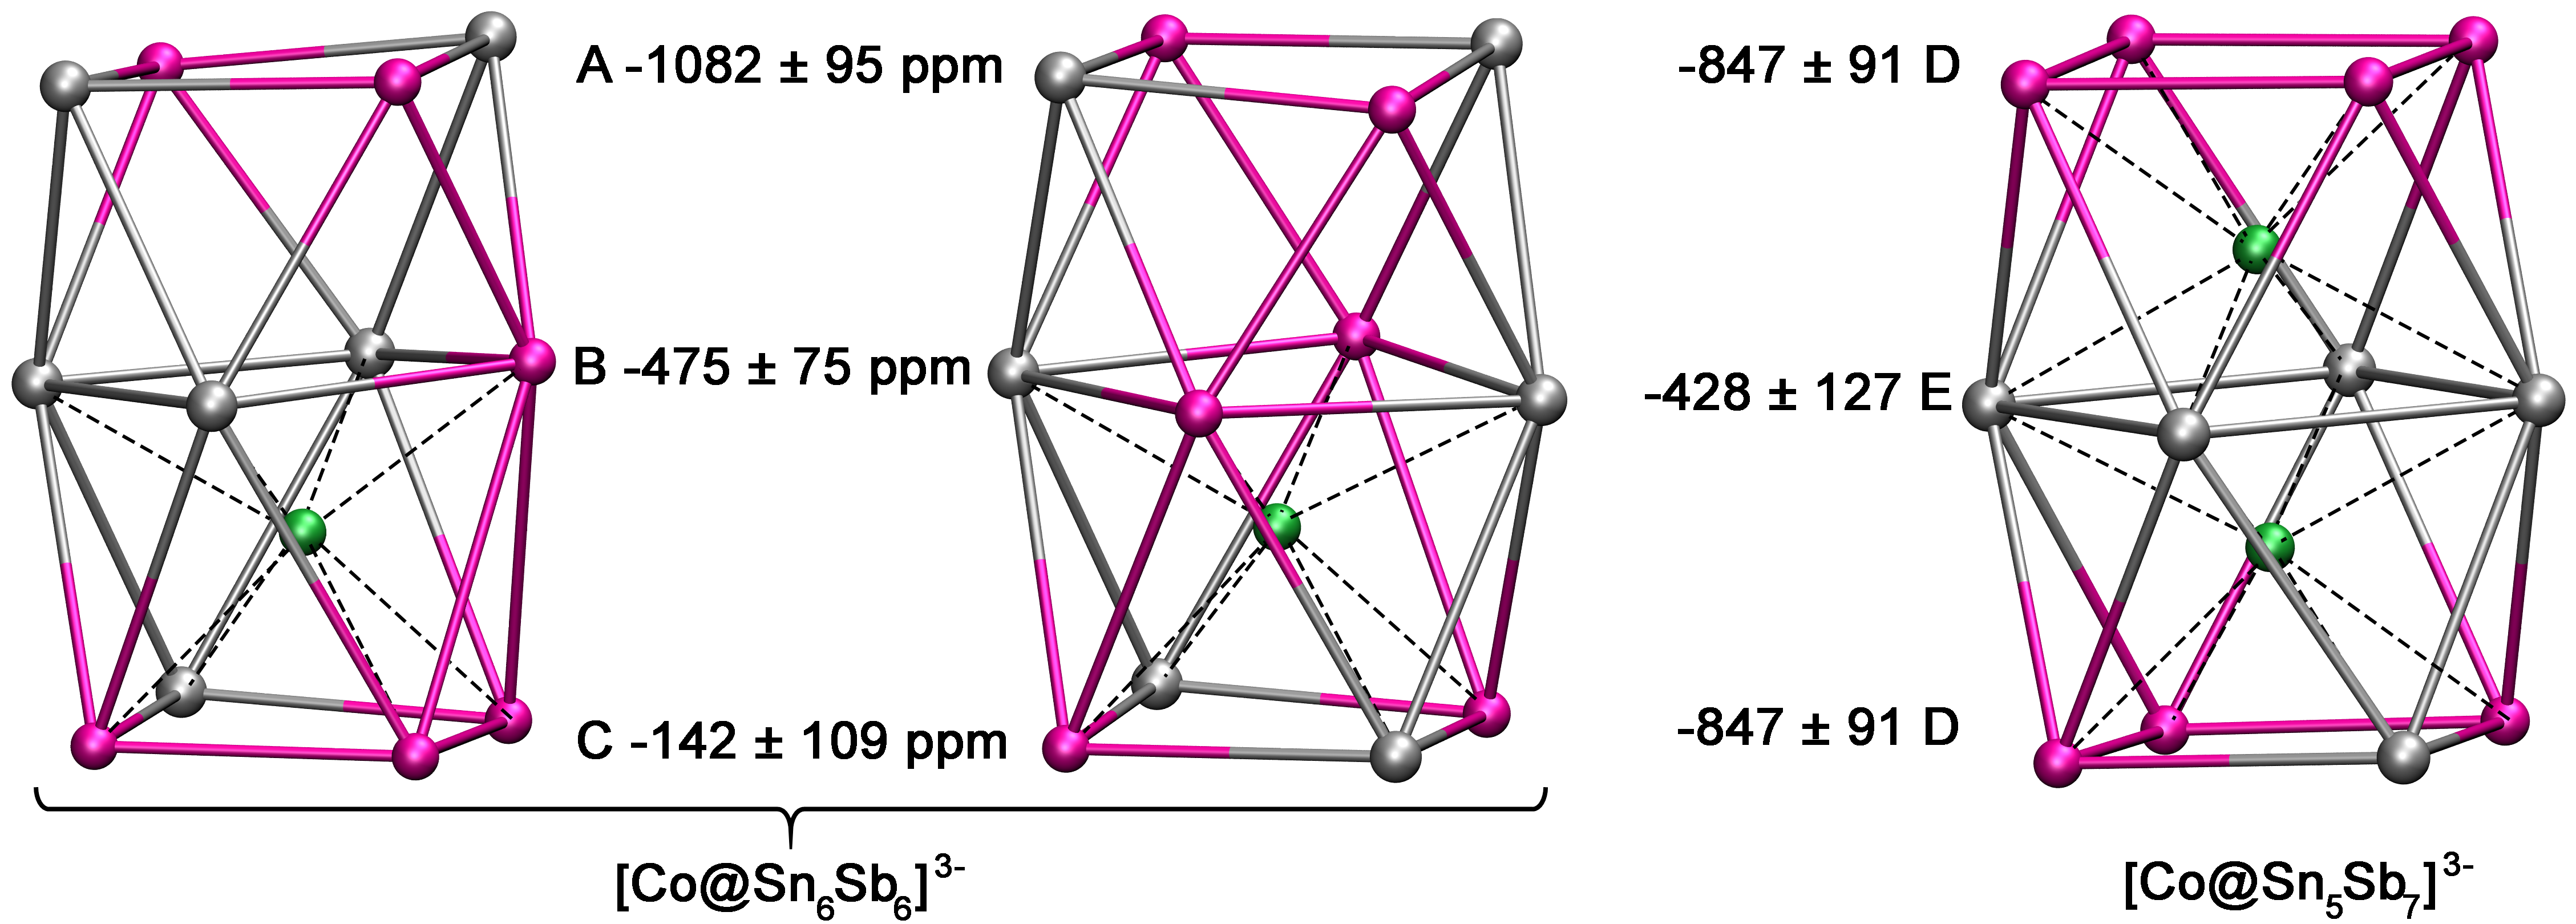
\includegraphics[width=1.0\textwidth]{coatsnsb}
	\captionsetup{figurewithin = chapter}
	\captionsetup{font=small, labelfont=bf}\caption[Strukturen von {[Co@Sn$_6$Sb$_6$]$^{3-}$ und [Co$_2$@Sn$_5$Sb$_7$]$^{3-}$}]{Strukturen der energetisch am tiefsten liegenden Isomere von [Co@Sn$_6$Sb$_6$]$^{3-}$ (links und Mitte) und [Co$_2$@Sn$_5$Sb$_7$]$^{3-}$ (rechts). Zusätzlich sind die gemittelten $^{119}$Sn-chemischen Verschiebungen sowie die zugehörigen Standardabweichungen für die viergliedrigen Ringe A--E in ppm angegeben. Dabei wurden alle Isomere in einem Energiebereich von \unit[10]{kJ/mol} relativ zum energetisch günstigsten Isomer einbezogen (siehe auch Tabelle \ref{tab:snnmrtab1} bis Tabelle \ref{tab:snnmrtab3}, Zinn=hellgrau, Antimon=magenta, Cobalt=grün).}
\label{abb:coatsnsb}
\end{figure}
\FloatBarrier
Aufgrund der vergleichsweise langen Zeitskala bei \ac{nmr}-Experimenten kann die Zuordnung der gemessenen Peaks auf die einzelnen Positionen durch intramolekularen Austausch zusätzlich erschwert werden. Das experimentelle $^{119}$Sn-\ac{nmr}-Spektrum des Einkristalls [K(crypt-222)]$_3$\{[Co@Sn$_6$Sb$_6$]$^{3-}$\}$_{0.83}$\{[Co$_2$@Sn$_5$Sb$_7$]$^{3-}$\}$_{0.17}\cdot$2dmf$\cdot$2tol gelöst in DMF-d$_7$ ist oben und das Spektrum von [K(crypt-222)]$_3$[Co$_2$@Sn$_5$Sb$_7$]$^{3-}$ ist unten in Abbildung \ref{abb:expsnnmr} gezeigt. Beide Spektren weisen mehrere scharfe Linien auf, wodurch hier von einem wenig dynamischen Verhalten in Lösung ausgegangen werden kann. Das obere Spektrum, welches beide Verbindungen beinhaltet, besitzt in den Bereichen D und E Signale, welche im Spektrum des reinen [K(crypt-222)]$_3$[Co$_2$@Sn$_5$Sb$_7$]$^{3-}$ deutlich an Intensität gewinnen und sich somit dieser Verbindung zuordnen lassen. Zusätzlich verschwinden dort die Signale aus den Bereichen A--C, wodurch diese Peaks der anderen Struktur zugeordnet werden können. 
\begin{figure}[ht!]
	\centering
	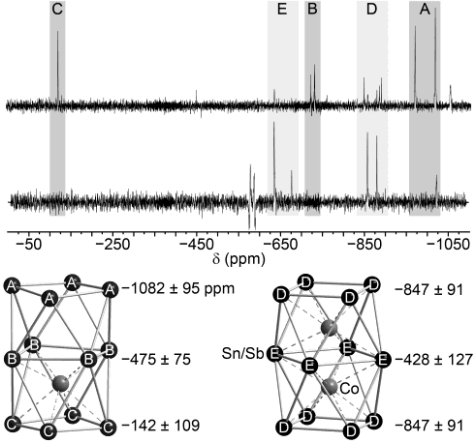
\includegraphics[width=1.0\textwidth]{snnmrspectra}
	\captionsetup{figurewithin = chapter}
	\captionsetup{font=small, labelfont=bf}\caption[{$^{119}$Sn-\ac{nmr}-Spektren von [Co@Sn$_6$Sb$_6$]$^{3-}$ und [Co$_2$@Sn$_5$Sb$_7$]$^{3-}$}]{Experimentelle $^{119}$Sn-\ac{nmr}-Spektren in DMF-d$_7$ von [K(crypt-222)]$_3$\{[Co@Sn$_6$Sb$_6$]$^{3-}$\}$_{0.83}$\{[Co$_2$@Sn$_5$Sb$_7$]$^{3-}$\}$_{0.17}\cdot$2dmf$\cdot$2tol \textsf{(a)} und [K(crypt-222)]$_3$[Co$_2$@Sn$_5$Sb$_7$]$^{3-}$ \textsf{(b)}.}
\label{abb:expsnnmr}
\end{figure}
\FloatBarrier

Für die Zuordnung der Peaks auf die atomaren Positionen wurden die $^{119}$Sn-chemischen Verschiebungen für die Isomere beider Clusteranionen mit einer relativen Energie von bis zu \unit[10]{kJ/mol} berechnet (siehe Tabelle \ref{tab:snnmrtab1} und \ref{tab:snnmrtab2}). Die Berechnungen wurden mit denselben Einstellungen wie bei der Optimierung der Strukturparameter durchgeführt, mit der Ausnahme, dass für Zinn die TZVPPall-Basis\supercite{ahlrichs2000contracted} verwendet wurde. Zur Vereinfachung wurden die chemischen Verschiebungen in den jeweiligen viergliedrigen Ringen A--E (siehe Abbildung \ref{abb:coatsnsb}) gemittelt. Die Nummerierung der Kohlenstoffatome ist in Abbildung \ref{abb:numbering} dargestellt. Da die einzelnen chemischen Verschiebungen sowohl innerhalb eines Ringes in einem Isomer als auch zwischen den einzelnen Isomeren variieren können, können mehrere Signale aus dem Spektrum einem Ring zugehörig sein. Wie deutlich zu erkennen ist, wird durch die \ac{dft}-Rechnung eine erhebliche Aufspaltung zwischen den äußeren Ringen A (\unit[$-$1082 $\pm$ 95]{ppm}) und C (\unit[$-$142 $\pm$ 109]{ppm}) erhalten. Der am höchsten gelegene Peak bei \unit[$-$119]{ppm} korreliert daher am besten mit Ring C, die beiden Peaks bei \unit[$-$970]{ppm} und \unit[$-$1018]{ppm} mit Ring A. Der verbleibende Peak bei \unit[$-$731]{ppm} kann folglich dem zentralen Ring B zugeordnet werden. Aus der Berechnung der chemischen Verschiebungen für [Co$_2$@Sn$_5$Sb$_7$]$^{3-}$ ergibt sich eine stärkere Abschirmung der Zinnatome in den äußeren Ringen D (\unit[$-$847 $\pm$ 91]{ppm}) als für die Zinnatome im zentralen Ring E (\unit[$-$428 $\pm$ 127]{ppm}). Dadurch erfolgt die Zuordnung der Peaks bei \unit[$-$634]{ppm} und \unit[$-$676]{ppm} zu Ring E und die der Peaks zwischen \unit[$-$849]{ppm} und \unit[$-$890]{ppm} zu den äußeren Ringen D. 
\vspace{20pt}
\begin{figure}[ht!]
	\centering
	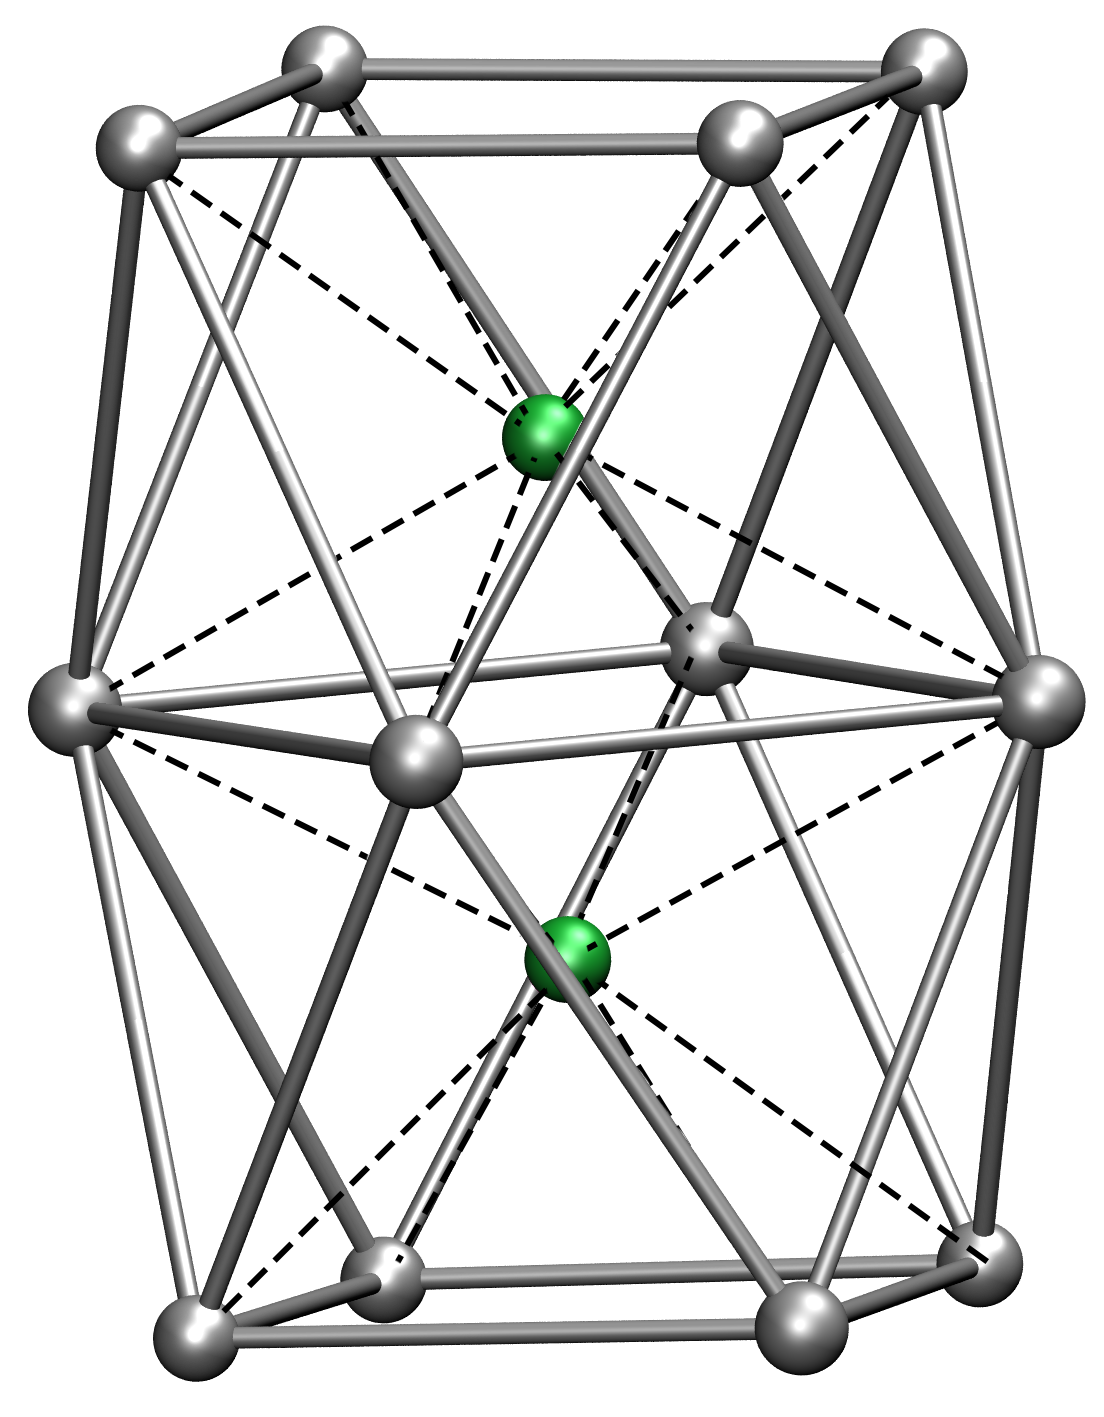
\includegraphics[width=0.4\textwidth]{numbering}
	\captionsetup{figurewithin = chapter}
	\captionsetup{font=small, labelfont=bf}\caption[Nummerierung der Atome in {[Co@Sn$_6$Sb$_6$]$^{3-}$} und {[Co$_2$@Sn$_5$Sb$_7$]$^{3-}$} ]{Nummerierung der Atome in den Clusteranionen [Co@Sn$_6$Sb$_6$]$^{3-}$ und [Co$_2$@Sn$_5$Sb$_7$]$^{3-}$. Für ersteres muss das Cobaltatom aus der oberen Hälfte entfernt werden.}
\label{abb:numbering}
\end{figure}
\vfill
\newpage

\begin{table}[ht!]
\captionsetup{tablewithin = chapter}
\captionsetup{font=small, labelfont=bf}
\captionabove[{$^{119}$Sn-chemische Verschiebungen von [Co@Sn$_6$Sb$_6$]$^{3-}$}]{Relative Energien $E$ und $^{119}$Sn-chemische Verschiebungen in Bezug auf SnMe$_4$ in ppm für die 10 stabilsten Isomere \textbf{A}--\textbf{J} von [Co@Sn$_6$Sb$_6$]$^{3-}$. Alle Berechnungen wurden mit TPSS/COSMO (mit Standardeinstellungen), der Basis dhf-TZVP für Co und Sb und der All-Elektronen-Basis TZVPPall für Sn durchgeführt. Die Nummerierungen beziehen sich auf Abbildung \ref{abb:numbering}.}
\resizebox{\textwidth}{!}{%
\begin{tabular}{crrrrrrrrrrrrr}
\hline \hline
  & $E$\text{\;\;\;\;} & \textbf{1} & \textbf{2} & \textbf{3} & \textbf{4} & \textbf{5} & \textbf{6} & \textbf{7} & \textbf{8} & \textbf{9} & \textbf{10} & \textbf{11} & \textbf{12} \\
  & kJ/mol  & & & & & & & & & & & &\\
  \hline
  \textbf{A} & 0 & & $-$1089 & & $-$1088 & & $-$538 & $-$522 & $-$404 & & & $-$335 &\\
  \textbf{B} & 2.6 & & $-$1122 & & $-$1125 & $-$542 & & $-$539 & & $-$137 & & $-$132 &\\
  \textbf{C} & 3.2 & & $-$1087 & $-$1153 & & $-$337 & $-$578 & & $-$462 & & & $-$117 &\\
  \textbf{D} & 3.9 & $-$1194 & & $-$960 & & $-$413 & $-$453 & $-$463 & & & & $-$147 &\\
  \textbf{E} & 4.2 & $-$1185 & & $-$943 & & & $-$436 & $-$466 & $-$426 & & & $-$165 &\\
  \textbf{F} & 8.1 & $-$1131 & & $-$904 & & $-$447 & $-$567 & & $-$349 & & & 40 &\\
  \textbf{G} & 11.2 & $-$1046 & & $-$1044 & & & $-$517 & & $-$519 & 99 & & 105 &\\
  \textbf{H} & 14.1 & & $-$1020 & & $-$1289 & $-$456 & $-$456 & & & $-$184 & & $-$184 &\\
  \textbf{I} & 16.6 & & & $-$1229 & $-$1476 & $-$241 & $-$591 & & $-$523 & & & 148 &\\
  \textbf{J} & 17.4 & $-$996 & & $-$999 & & $-$407 & $-$404 & & & 23 & & 35 &\\
\end{tabular}}
\label{tab:snnmrtab1}
\end{table}

\begin{table}[ht!]
\captionsetup{tablewithin = chapter}
\captionsetup{font=small, labelfont=bf}
\captionabove[{$^{119}$Sn-chemische Verschiebungen von [Co$_2$@Sn$_5$Sb$_7$]$^{3-}$}]{Relative Energien $E$ und $^{119}$Sn-chemische Verschiebungen in Bezug auf SnMe$_4$ in ppm für die 15 stabilsten Isomere \textbf{A}--\textbf{O} von [Co$_2$@Sn$_5$Sb$_7$]$^{3-}$. Alle Berechnungen wurden mit TPSS/COSMO (mit Standardeinstellungen), der Basis dhf-TZVP für Co und Sb und der All-Elektronen-Basis TZVPPall für Sn durchgeführt. Die Nummerierungen beziehen sich auf Abbildung \ref{abb:numbering}.}
\resizebox{\textwidth}{!}{%
\begin{tabular}{crrrrrrrrrrrrr}
\hline \hline
  & $E$\text{\;\;\;\;} & \textbf{1} & \textbf{2} & \textbf{3} & \textbf{4} & \textbf{5} & \textbf{6} & \textbf{7} & \textbf{8} & \textbf{9} & \textbf{10} & \textbf{11} & \textbf{12} \\
  & kJ/mol  & & & & & & & & & & & &\\
  \hline
  \textbf{A} & 0 & & & & & $-$387 & $-$527 & $-$523 & $-$383 & & & $-$993 &\\
  \textbf{B} & 3.7 & & & $-$715 & & $-$238 & $-$628 & & $-$302 & & & $-$715 &\\
  \textbf{C} & 6.5 & & $-$930 & & & $-$373 & $-$615 & & $-$305 & & & $-$807 &\\
  \textbf{D} & 7.0 & & $-$853 & & & $-$483 & & $-$482 & $-$219 & & & $-$852 &\\
  \textbf{E} & 8.9 & & & $-$875 & & & $-$567 & $-$463 & $-$347 & & & $-$875 &\\
  \textbf{F} & 10.3 & & & & & $-$467 & $-$367 & $-$455 & & $-$727 & & $-$777 &\\
  \textbf{G} & 10.6 & & & & $-$945 & & $-$475 & $-$498 & $-$481 & & & $-$938 &\\
  \textbf{H} & 11.8 & & $-$619 & & $-$693 & & $-$635 & & $-$416 & & & $-$764&\\
  \textbf{I} & 12.0 & $-$968 & & & & $-$493 & $-$365 & $-$422 & & & & $-$1026 &\\
  \textbf{J} & 15.1 & $-$857 & & $-$537 & & & $-$589 & & $-$439 & & & $-$890 &\\
  \textbf{K} & 15.4 & & $-$670 & & $-$676 & & $-$488 & $-$486 & & & & $-$837 &\\
  \textbf{L} & 15.7 & & $-$648 & & $-$648 & $-$341 & & & $-$341 & & & $-$689 &\\
  \textbf{M} & 16.2 & $-$850 & & $-$508 & & $-$342 & $-$486 & & & & & $-$902 &\\
  \textbf{N} & 17.7 & & $-$654 & & $-$723 & $-$335 & $-$527 & & & & & $-$816 &\\
  \textbf{O} & 21.6 & & $-$616 & & $-$552 & & & & $-$497 & $-$545 & & $-$624 &\\
\end{tabular}}
\label{tab:snnmrtab2}
\end{table}
\vfill
\newpage
\begin{table}[ht!]
\captionsetup{tablewithin = chapter}
\captionsetup{font=small, labelfont=bf}
\captionabove[{Statistische Werte der chemischen Verschiebungen von [Co@Sn$_6$Sb$_6$]$^{3-}$ und [Co$_2$@Sn$_5$Sb$_7$]$^{3-}$}]{Statistische Werte (Minimum, Maximum, Mittelwert (MW) und Standardabweichung (SA)) der chemischen Verschiebungen für die Isomere von [Co@Sn$_6$Sb$_6$]$^{3-}$ und [Co$_2$@Sn$_5$Sb$_7$]$^{3-}$. Einbezogen wurden alle Isomere mit relativen Energien kleiner als \unit[10]{kJ/mol}. Die Nummerierungen beziehen sich auf Abbildung \ref{abb:numbering}.}
\resizebox{\textwidth}{!}{%
\begin{tabular}{cc|cccc|cccc|cccc}
\hline \hline
  & & \multicolumn{4}{c|}{\textbf{1--4}} & \multicolumn{4}{c|}{\textbf{5--8}} & \multicolumn{4}{c}{\textbf{9--12}} \\
  & Strukturen  & Min & Max & MW & SA & Min & Max & MW & SA & Min & Max & MW & SA\\
  \hline
  [Co@Sn$_6$Sb$_6$]$^{3-}$ & A--F & $-$1194 & $-$904 & $-$1082 & 95 & $-$578 & $-$357 & $-$475 & 75 & $-$335 & 40 & $-$142 & 109\\
  & & & & & & & & & & & & & \\
  & & & & & & \multicolumn{4}{c|}{\textbf{5--8}} & \multicolumn{4}{c}{\textbf{1--4, 9--12}}\\
  \hline
  [Co$_2$@Sn$_5$Sb$_7$]$^{3-}$ & A--E & & & & & $-$628 & $-$219 & $-$428 & 127 & $-$993 & $-$715 & $-$847 & 91\\
\end{tabular}}
\label{tab:snnmrtab3}
\end{table}
\subsection{\texorpdfstring{$^{31}$P}{31P}-chemische Verschiebungen in Phospor-NHCs}
Um ein besseres Verständnis der chemischen Verschiebung in einer Reihe von Phosphor-N-Heterocyclischen-Carben-(\acs{nhc}-)Verbindungen \supercite{lemp2017nhc} zu erhalten, wurden die chemischen Abschirmungskonstanten für die in den Abbildung \ref{abb:cvhabc} bis \ref{abb:cvhfg} gezeigten Verbindungen auf \ac{dft}-Niveau berechnet. Die in Tabelle \ref{tab:cvhtab1} gelisteten Werte wurden unter Verwendung des PBE-Funktionals\supercite{perdew1996generalized} und der Basis def2-TZVP\supercite{weigend2005balanced} erhalten. Zuvor wurden die Strukturparameter der entsprechenden Verbindungen auf demselben Niveau optimiert, wobei zusätzlich Grimmes Dispersionskorrektur D3\supercite{grimme2010consistent,grimme2011effect} verwendet wurde. Weiterhin wurde das \ac{cosmo}\supercite{klamt1993cosmo} mit einer Dielektrizitätskonstante von 2.28 verwendet, um das experimentelle Lösungsmittel Benzol zu simulieren. Zusätzlich zu den berechneten absoluten Abschirmungskonstanten sind in Tabelle \ref{tab:cvhtab1} sowohl die experimentellen $^{31}$P- und $^{13}$C-(Carben-Kohlenstoffatom-)chemische Verschiebungen als auch simulierte chemische Verschiebungen aus den berechneten Werten angegeben: $\delta=\sigma_0-\sigma$. $\sigma_0$ wurde durch Minimieren der Abweichung zwischen den experimentellen Verschiebungen und den berechneten Abschirmungskonstanten bestimmt. Für die $^{13}$C-chemischen Verschiebungen wird damit eine Übereinstimmung zwischen Experiment und Rechnung bis auf etwa \unit[2]{ppm} erhalten und die Reihenfolge korrekt wiedergegeben. Die $^{31}$P-chemischen Verschiebungen sind aufgrund ihres größeren Bereichs der chemischen Verschiebung deutlich problematischer. Fehler von \unit[30]{ppm} sind keine Seltenheit, wie bereits gezeigt wurde.\supercite{latypov2015quantum,reiter2017calculation} Abgesehen von der Verbindung $[$SIMesPGa$^\textit{t}$Bu$_2]_2$ ( SIMes=1,3-bis(2,4,6-tri\-me\-thyl\-phe\-nyl)imi\-da\-zo\-lin-2-yli\-den) liegen die anderen Verbindungen damit also in einem akzeptablen Bereich. Die Trends in der $^{31}$P-chemischen Verschiebung werden korrekt wiedergegeben und auch die vergleichsweise niedrige Abschirmung in K(SIMesP)$_3$Al$^\textit{t}$Bu wird durch die Berechnung bestätigt. Diese Befunde sind vom verwendeten Funktional unabhängig, wie Tabelle \ref{tab:cvhtab2} zeigt. Neben den berechneten Werten mit dem PBE-Funktional sind dort auch die Ergebnisse mit den Funktionalen PBE0\supercite{adamo1999toward}, BP86\supercite{perdew1986density,becke1988density} und B3LYP\supercite{becke1993density,lee1988development,stephens1994ab} sowie einer Hartree-Fock-Rechnung aufgelistet. Grundlage für diese Berechnungen waren jedoch die experimentellen Strukturen.

\begin{table}[ht!]
\captionsetup{tablewithin = chapter}
\captionsetup{font=small, labelfont=bf}
\captionabove[Vergleich spektroskopischer und struktureller Daten für Phosphor-\\NHCs]{Vergleich spektroskopischer und struktureller Daten für SIMesPH, IMesPH, $[$SIMesPGa$^\textit{t}$Bu$_2]_2$, SIMesP(Ga$^\textit{t}$Bu$_2$)$_2$Cl, K(SIMesP)$_3$Al$^\textit{t}$Bu, SIMesPH$^\textit{t}$Bu$_2$GaCl und SIMesPH$^\textit{t}$Bu$_2$AlCl.}
\resizebox{\textwidth}{!}{%
\begin{tabular}{lrrrrrrrr}
\hline \hline
Verbindung & \multicolumn{3}{c}{$^{31}$P / ppm} & \multicolumn{3}{c}{$^{13}$C (Carbenkohlenstoff) / ppm} & \multicolumn{2}{c}{P--C Abstand/ pm}\\
 & gemessen & \multicolumn{2}{c}{berechnet} & gemessen & \multicolumn{2}{c}{berechnet} &Röntgenstruktur & berechnet\\
 & & sim. $\delta ^{31}$P & $\sigma ^{31}$P & & sim. $\delta ^{13}$C & $\sigma ^{13}$C & & \\
 \hline
 SIMesPH & $-$127.2 & $-$157 & 433 & 191.0 & 192 & $-$3 & 174.6(2) & 175.3\\
 IMesPH & $-$147.3 & $-$178 & 454 & 180.0 & 178 & 11 & 174.7(2) & 176.1\\
 $[$SIMesPGa$^\textit{t}$Bu$_2]_2$ & $-$113.2 & $-$57 & 333 & & 182 & 7 & 174.4(2) & 175.6\\
 SIMesP(Ga$^\textit{t}$Bu$_2$)$_2$Cl & $-$122.6 & $-$104 & 380 & 183.3 & 181 & 8 & 175.4(1) & 175.3\\
 K(SIMesP)$_3$Al$^\textit{t}$Bu & $-$61.2 & $-$54 & 330 & & 185 & 4 & 175.3(2) & 175.8\\
 SIMesPH$^\textit{t}$Bu$_2$GaCl & $-$148.8 & $-$163 & 439 & 188.5 & 191 & $-$2 & 179.8(2) & 179.4\\
 SIMesPH$^\textit{t}$Bu$_2$AlCl & $-$151.0 & $-$157 & 433 & 187.9 & 190 & $-$1 & 180.1(2) & 179.5
\end{tabular}}
\label{tab:cvhtab1}
\end{table}

\begin{table}[ht!]
\captionsetup{tablewithin = chapter}
\captionsetup{font=small, labelfont=bf}
\captionabove[$^{31}$P-chemische Verschiebungen/Abschirmungen für Phosphor-NHCs mit unterschiedlichen Funktionalen]{$^{31}$P-chemische Verschiebungen/Abschirmungen für SIMesPH, IMesPH, $[$SIMesPGa$^\textit{t}$Bu$_2]_2$, SIMesP(Ga$^\textit{t}$Bu$_2$)$_2$Cl, K(SIMesP)$_3$Al$^\textit{t}$Bu, SIMesPH$^\textit{t}$Bu$_2$GaCl und SIMesPH$^\textit{t}$Bu$_2$AlCl mit unterschiedlichen Funktionalen. Die Spalte \glqq PBE, opt\grqq{} enthält die berechneten Werte für optimierte Strukturparameter. Alle Werte in den darauf folgenden Spalten wurden auf Grundlage der experimentellen Strukturparametern berechnet und sind in ppm angegeben.}
\resizebox{\textwidth}{!}{%
\begin{tabular}{lrrrrrrrrrrrrr}
\hline \hline
Verbindung &gemessen &\multicolumn{2}{c}{PBE, opt} &\multicolumn{2}{c}{PBE} &\multicolumn{2}{c}{BP86} &\multicolumn{2}{c}{B3-LYP} &\multicolumn{2}{c}{PBE0} &\multicolumn{2}{c}{HF}\\
& & $\delta ^{31}$P & $\sigma ^{31}$P & $\delta ^{31}$P & $\sigma ^{31}$P & $\delta ^{31}$P & $\sigma ^{31}$P & $\delta ^{31}$P & $\sigma ^{31}$P & $\delta ^{31}$P & $\sigma ^{31}$P & $\delta ^{31}$P & $\sigma ^{31}$P\\
\hline
SIMesPH &$-$127.2 &$-$157 &433 &$-$164 &455 &$-$165 &450 &$-$163 &443 &$-$155 &465 &$-$140 &491\\
IMesPH &$-$147.3 &$-$178 &454 &$-$137 &428 &$-$138 &423 &$-$136 &416 &$-$133 &443 &$-$121 &472\\
$[$SIMesPGa$^\textit{t}$Bu$_2]_2$ &$-$113.2 &$-$57  &333 &$-$59  &350 &$-$58  &343 &$-$61  &341 &$-$68  &378 &$-$94  &445\\
SIMesP(Ga$^\textit{t}$Bu$_2$)$_2$Cl &$-$122.6 &$-$104 &380 &$-$109 &400 &$-$107 &392 &$-$111 &391 &$-$117 &427 &$-$137 &488\\
K(SIMesP)$_3$Al$^\textit{t}$Bu &$-$61.2  &$-$54  &330 &$-$77  &368 &$-$77  &362 &$-$79  &359 &$-$83  &393 &$-$99  &450\\
SIMesPH$^\textit{t}$Bu$_2$GaCl &$-$148.8 &$-$163 &439 &$-$162 &453 &$-$162 &447 &$-$162 &442 &$-$160 &470 &$-$144 &495\\
SIMesPH$^\textit{t}$Bu$_2$AlCl &$-$151.0   &$-$157 &433 &$-$163 &454 &$-$164 &449 &$-$161 &441 &$-$158 &468 &$-$137 &488\\
\end{tabular}}
\label{tab:cvhtab2}
\end{table}

\FloatBarrier

Es zeigte sich, dass die Unterschiede in den chemischen Abschirmungskonstanten der einzelnen Verbindungen im Wesentlichen aufgrund des paramagnetischen Beitrages zustande kommen. In diesem Beitrag ist die Response der Elektronendichte auf das äußere Magnetfeld enthalten, im diamagnetischen Beitrag hingegen die Elektronendichte selbst. Erwartungsgemäß ist der diamagnetische Beitrag in allen untersuchten Verbindungen sehr ähnlich und liegt zwischen \unit[960]{ppm} und \unit[967]{ppm}. Dieser Befund führt zu der Schlussfolgerung, dass alle weiteren Untersuchungen, welche auf der Elektronendichte basieren (wie beispielsweise Populationsanalysen), nicht dafür geeignet sind, die Unterschiede in den einzelnen Abschirmungskonstanten zu erklären. Eine erhöhte Elektronendichte und eine damit einhergehende stärker negative Partialladung am Phosphoratom führt also nicht zwangsläufig zu einer stärkeren Abschirmung. Der paramagnetische Beitrag hingegen ist anfällig auf Änderungen in der Geometrie und der elektronischen Struktur der jeweiligen Verbindung. Dies wird beispielsweise beim Vergleich von SIMesPH und IMesPH deutlich, welche eine chemische Verschiebung von etwa \unit[20]{ppm} zueinander aufweisen. Die beiden Strukturen unterscheiden sich lediglich durch die Anzahl der Wasserstoffatome an den Kohlenstoffatomen im fünfgliedrigen Ring. Die große Änderung der elektronischen Struktur wird auch bei der Rotation der C--P-Bindung offensichtlich. Die $^{31}$P-Abschirmungskonstante in den jeweiligen Übergangszuständen liegt um ca. \unit[60]{ppm} höher als die des zugehörigen Grundzustandes. Um den rein elektronischen Einfluss auf die Abschirmungskonstanten der Grundzustände von SIMesPH und IMesPH (IMes=1,3-bis(2,4,6-tri\-me\-thyl\-phe\-nyl)imi\-da\-zol-2-yli\-den) weiter zu untersuchen, wurde in der Verbindung SIMesPH jeweils ein Wasserstoffatom an den Kohlenstoffatomen entfernt und die Positionen aller anderen Atome beibehalten. Die erhaltene Abschirmungskonstante liegt bei etwa \unit[444]{ppm} und damit genau in der Mitte der beiden Verbindungen. All diese Unterschiede basieren allein auf dem paramagnetischen Beitrag. Der diamagnetische Beitrag liegt in allen Fällen bei \unit[962]{ppm}.
Diese hohe Sensibilität mag der ausschlaggebende Grund für den Unterschied zwischen der experimentellen und berechneten chemischen Verschiebung in $[$SIMesPGa$^\textit{t}$Bu$_2]_2$ sein. Diese Verbindung unterscheidet sich von SIMesP(Ga$^\textit{t}$Bu$_2$)$_2$Cl nur durch das Ersetzen eines SIMesP-Restes durch ein Chloratom. Wird erneut die Geometrie von $[$SIMesPGa$^\textit{t}$Bu$_2]_2$ genommen und dieser Austausch durchgeführt, so wird bei der Nachoptimierung der Position des Chloratoms unter Beibehaltung der restlichen Strukturparameter eine $^{31}$P-Abschirmungskonstante von \unit[336]{ppm} erhalten. Dieser Wert ist fast identisch mit dem aus der Verbindung $[$SIMesPGa$^\textit{t}$Bu$_2]_2$ und unterscheidet sich daher deutlich vom Wert der Verbindung mit optimierten Strukturparametern (SIMesP(Ga$^\textit{t}$Bu$_2$)$_2$Cl, \unit[380]{ppm}). Die Änderung der Strukturparameter hat daher eindeutig einen großen Einfluss auf den paramagnetischen Beitrag. Die Ähnlichkeit in der gemessenen Abschirmung von $[$SIMesPGa$^\textit{t}$Bu$_2]_2$ und SIMesP(Ga$^\textit{t}$Bu$_2$)$_2$Cl ist daher überraschender als die vergleichsweise kleine gemessene und berechnete Verschiebung in der Verbindung K(SIMesP)$_3$Al$^\textit{t}$Bu.

Zur weiteren Untersuchung dieser Erkenntnisse wurde eine Zerlegung des diamagnetischen und paramagnetischen Teils der chemischen Abschirmungskonstante in einzelne Orbitalbeiträge exemplarisch für SIMesP(Ga$^\textit{t}$Bu$_2$)$_2$Cl unternommen, wie es beispielsweise von Wiberg \textit{et al.}\supercite{wiberg1998nmr} vorgeschlagen wurde. Im Detail sind die Werte in Tabelle \ref{tab:cvhzerlegung} im Anhang zu finden. Zusätzlich sind dort in Abbildung \ref{abb:modec} die \acp{mo} gezeigt, welche den größten Beitrag liefern. Erwartungsgemäß dominieren die inneren Orbitale des Phosphoratoms den diamagnetischen Beitrag. Hauptsächlich sind dies das 1$s$ mit ca. \unit[500]{ppm} aber auch die 2$s$- und 2$p$-Orbitale, welche jeweils einen Beitrag von ca. \unit[100]{ppm} liefern. Der größte Beitrag für den paramagnetischen Anteil kommt mit ca. \unit[$-$180]{ppm} von der C--P$\pi$-Bindung. Allerdings gibt es viele Orbitale, welche ebenfalls einen Beitrag von mehr als \unit[10]{ppm} liefern. Die vergleichsweise kleinen Unterschiede in der chemischen Abschirmung der untersuchten Verbindungen lassen sich damit daher nicht weiter auflösen.

\begin{figure}[ht!]
	\centering
	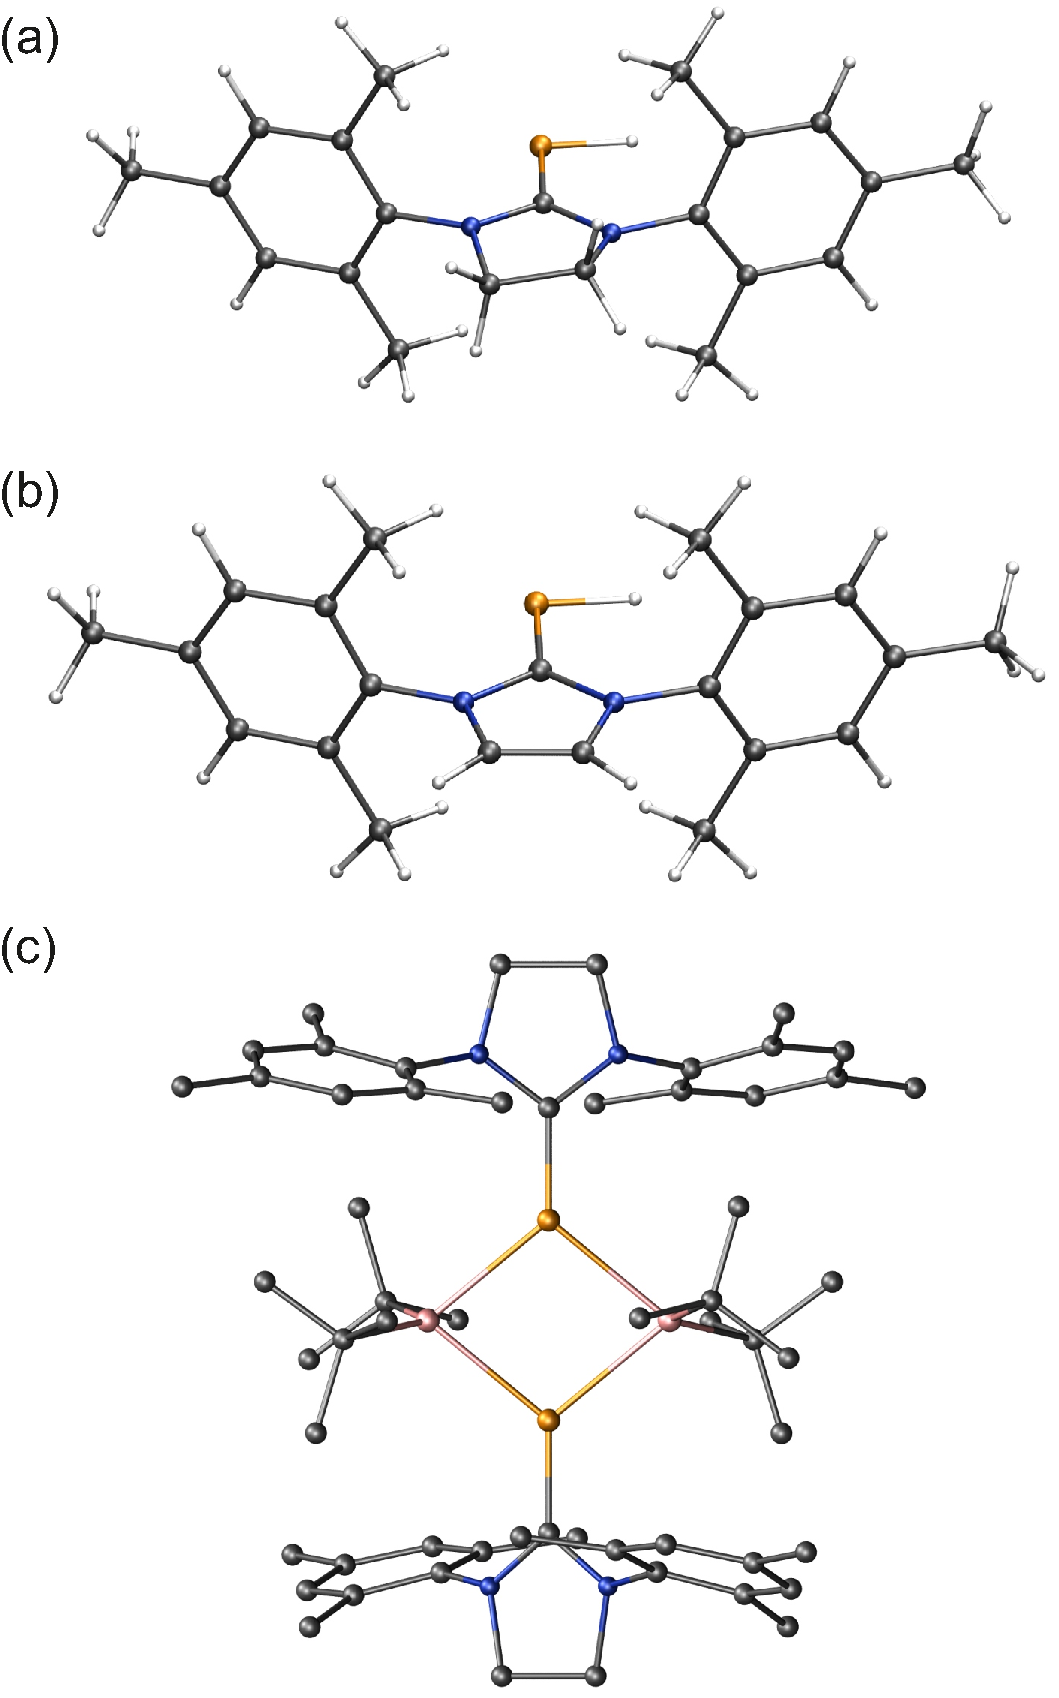
\includegraphics[width=0.65\textwidth]{cvhabc}
	\captionsetup{figurewithin = chapter}
	\captionsetup{font=small, labelfont=bf}\caption[{Abbildung von SIMesPH, IMesPH und $[$SIMesPGa$^\textit{t}$Bu$_2]_2$}]{ SIMesPH, SIMes=1,3-bis(2,4,6-tri\-me\-thyl\-phe\-nyl)imi\-da\-zo\-lin-2-yli\-den \textsf{(a)}. IMesPH, IMes=1,3-bis(2,4,6-tri\-me\-thyl\-phe\-nyl)imi\-da\-zol-2-yli\-den \textsf{(b)}. $[$SIMesPGa$^\textit{t}$Bu$_2]_2$ \textsf{(c)} (Kohlenstoff=grau, Wasserstoff=weiß, Stickstoff=blau, Phosphor=orange und Gallium=rosa). Die Wasserstoffatome wurden bei \textsf{(c)} zur besseren Veranschaulichung weggelassen.}
\label{abb:cvhabc}
\end{figure}

\begin{figure}[ht!]
	\centering
	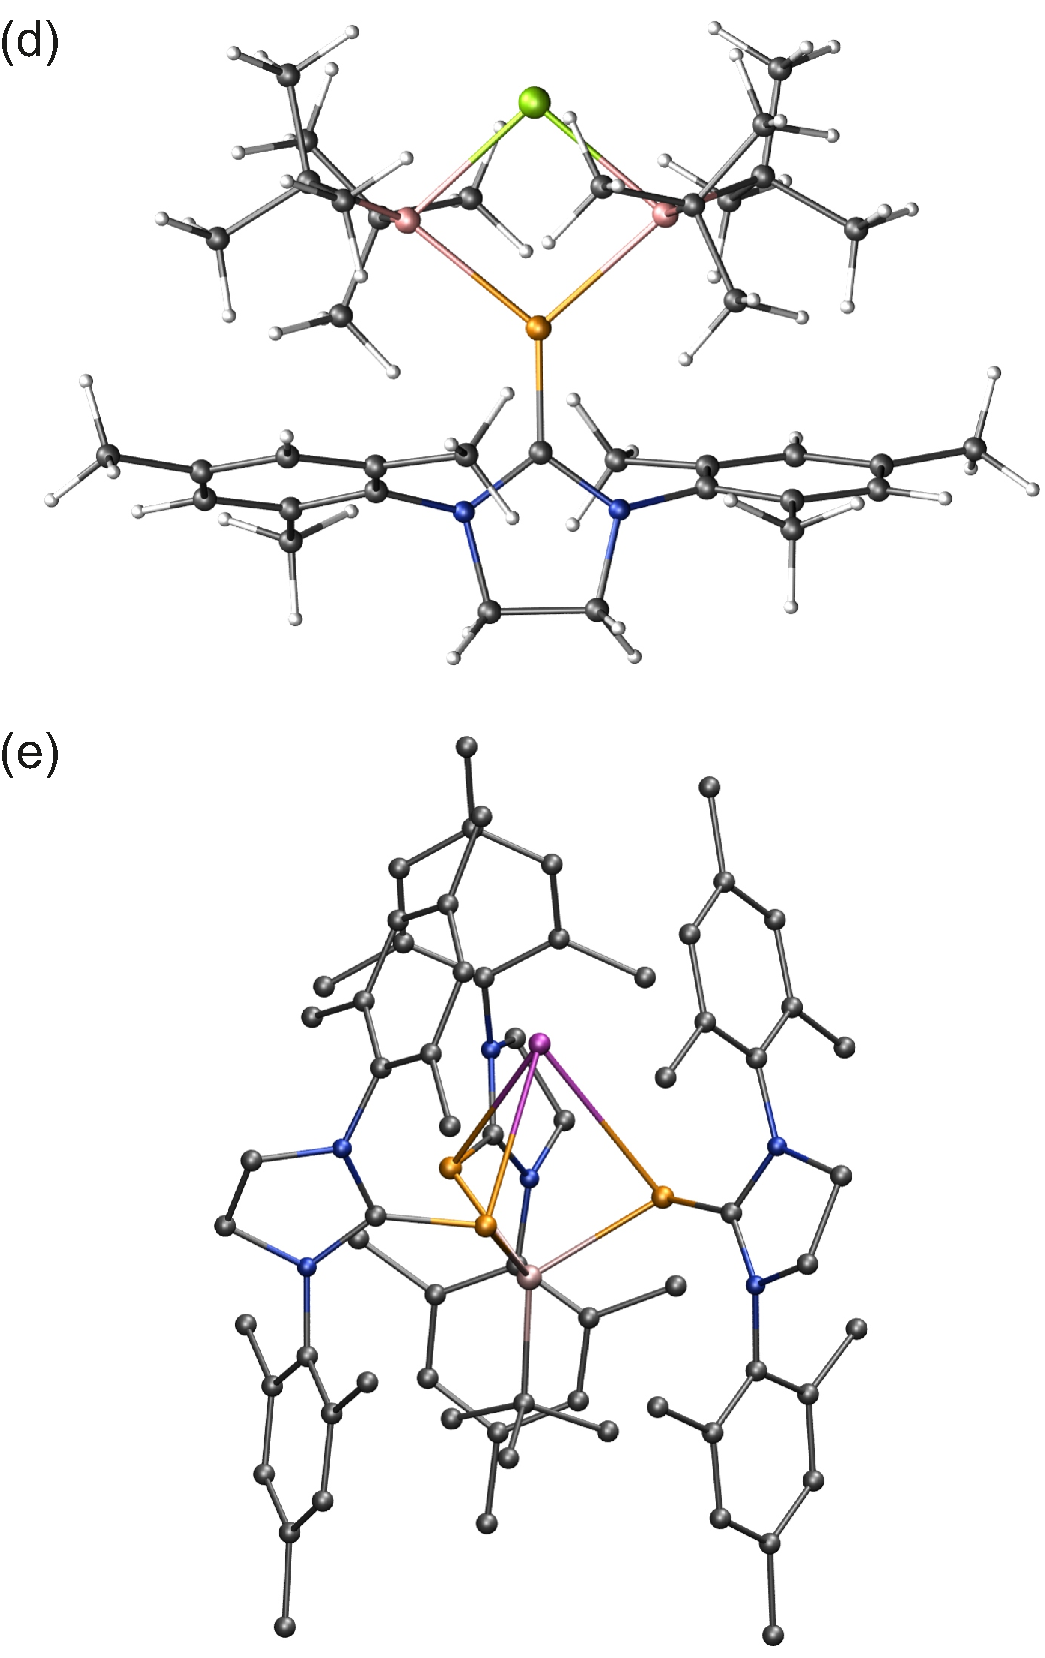
\includegraphics[width=0.65\textwidth]{cvhde}
	\captionsetup{figurewithin = chapter}
	\captionsetup{font=small, labelfont=bf}\caption[{Abbildung von SIMesP(Ga$^\textit{t}$Bu$_2$)$_2$Cl und K(SIMesP)$_3$Al$^\textit{t}$Bu}]{SIMesP(Ga$^\textit{t}$Bu$_2$)$_2$Cl \textsf{(d)}. K(SIMesP)$_3$Al$^\textit{t}$Bu \textsf{(e)} (Kohlenstoff=grau, Wasserstoff=weiß, Stickstoff=blau, Phosphor=orange, Gallium=rosa, Chlor=grün, Kalium=lila und Aluminium=hellrosa). Die Wasserstoffatome wurden bei \textsf{(e)} zur besseren Veranschaulichung weggelassen.}
\label{abb:cvhde}
\end{figure}

\begin{figure}[ht!]
	\centering
	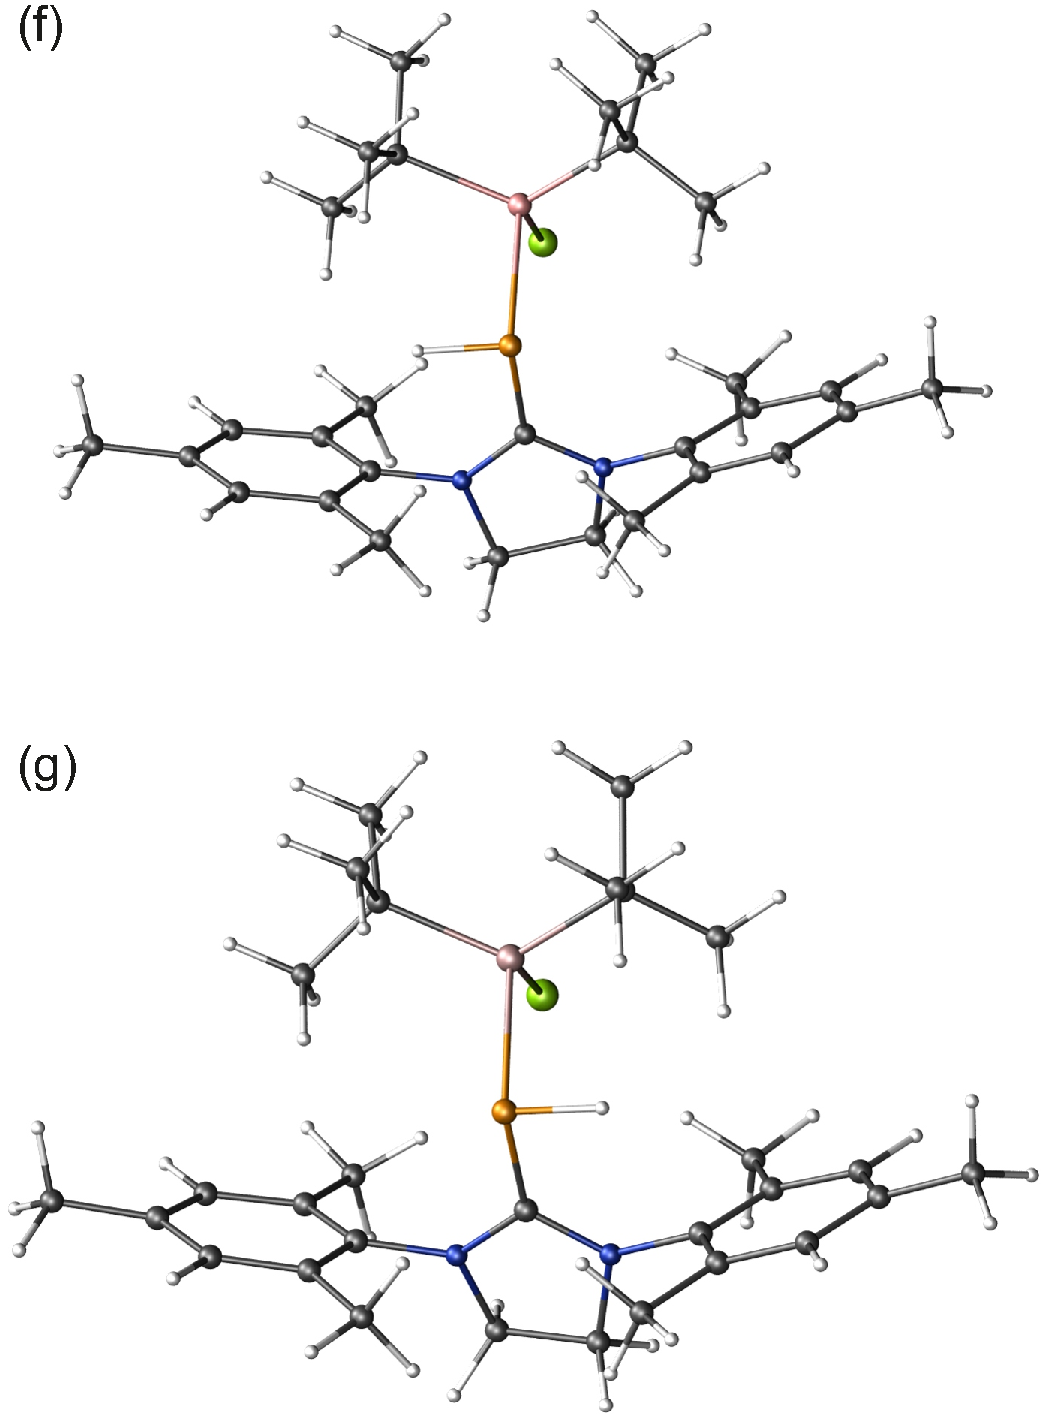
\includegraphics[width=0.6\textwidth]{cvhfg}
	\captionsetup{figurewithin = chapter}
	\captionsetup{font=small, labelfont=bf}\caption[{Abbildung von SIMesPH$^\textit{t}$Bu$_2$GaCl und SIMesPH$^\textit{t}$Bu$_2$AlCl}]{SIMesPH$^\textit{t}$Bu$_2$GaCl \textsf{(f)}. SIMesPH$^\textit{t}$Bu$_2$AlCl \textsf{(g)} (Kohlenstoff=grau, Wasserstoff=weiß, Stickstoff=blau, Phosphor=orange, Gallium=rosa, Aluminium=hellrosa und Chlor=grün).}
\label{abb:cvhfg}
\end{figure}


%\begin{figure}[ht!]
%	\centering
%	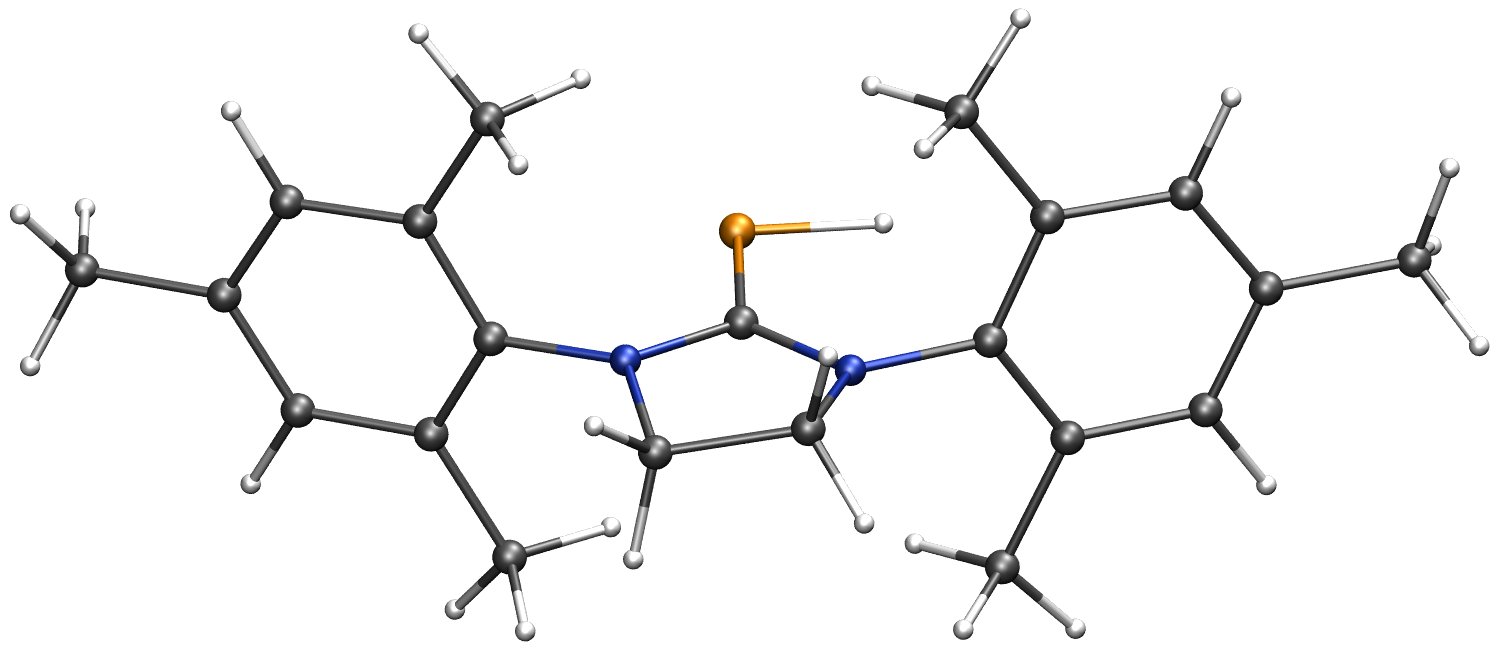
\includegraphics[width=0.6\textwidth]{1}
%	\captionsetup{figurewithin = chapter}
%	\captionsetup{font=small, labelfont=bf}\caption[Abbildung von SIMesPH]{Abbildung von SIMesPH, SIMes=1,3-bis(2,4,6-tri\-me\-thyl\-phe\-nyl)imi\-da\-zo\-lin-2-yli\-den (Kohlenstoff=grau, Wasserstoff=weiß, Stickstoff=blau und Phosphor=orange).}
%\label{abb:cvh1}
%\end{figure}
%
%\begin{figure}[ht!]
%	\centering
%	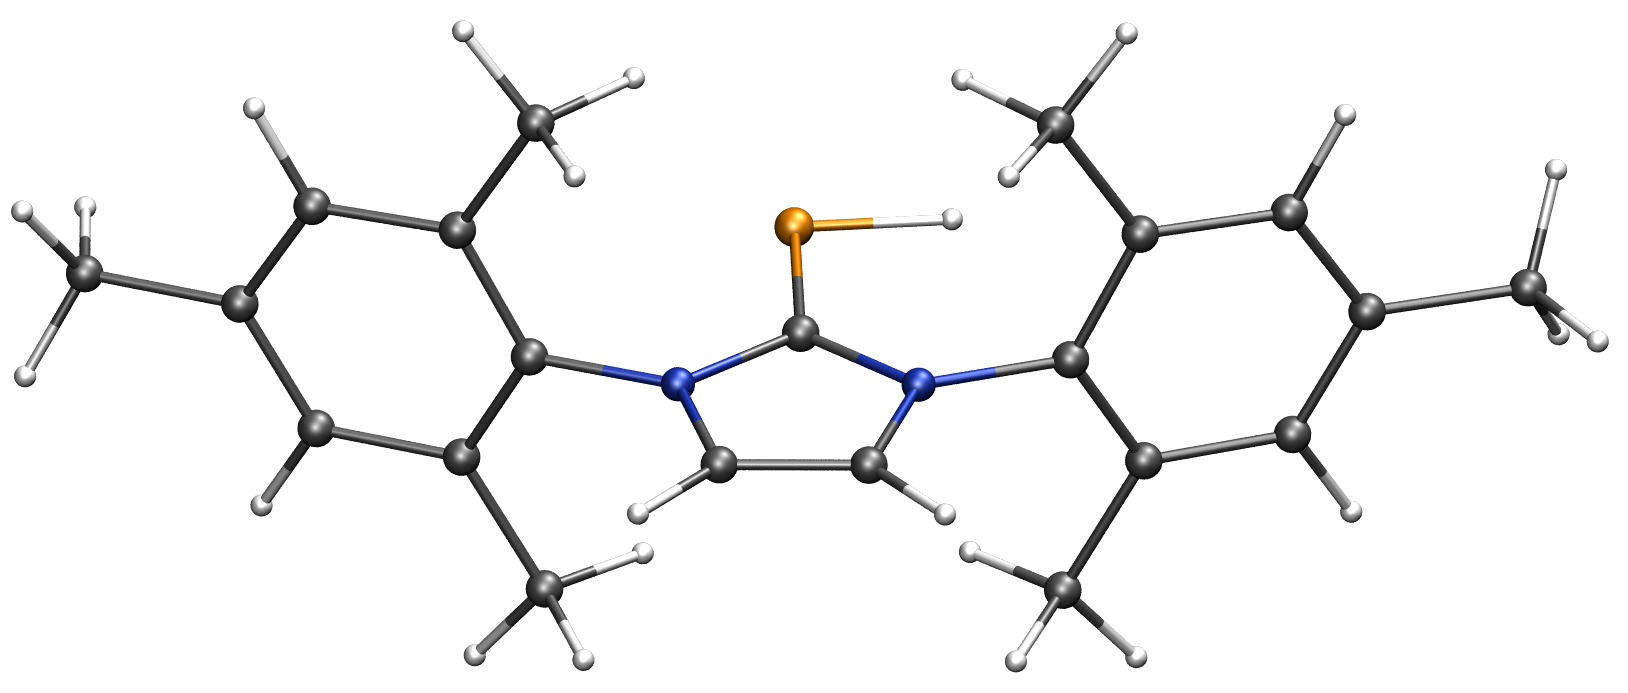
\includegraphics[width=0.6\textwidth]{2}
%	\captionsetup{figurewithin = chapter}
%	\captionsetup{font=small, labelfont=bf}\caption[Abbildung von IMesPH]{Abbildung von IMesPH, IMes=1,3-bis(2,4,6-tri\-me\-thyl\-phe\-nyl)imi\-da\-zol-2-yli\-den (Kohlenstoff=grau, Wasserstoff=weiß, Stickstoff=blau und Phosphor=orange).}
%\label{abb:cvh2}
%\end{figure}
%
%\begin{figure}[ht!]
%	\centering
%	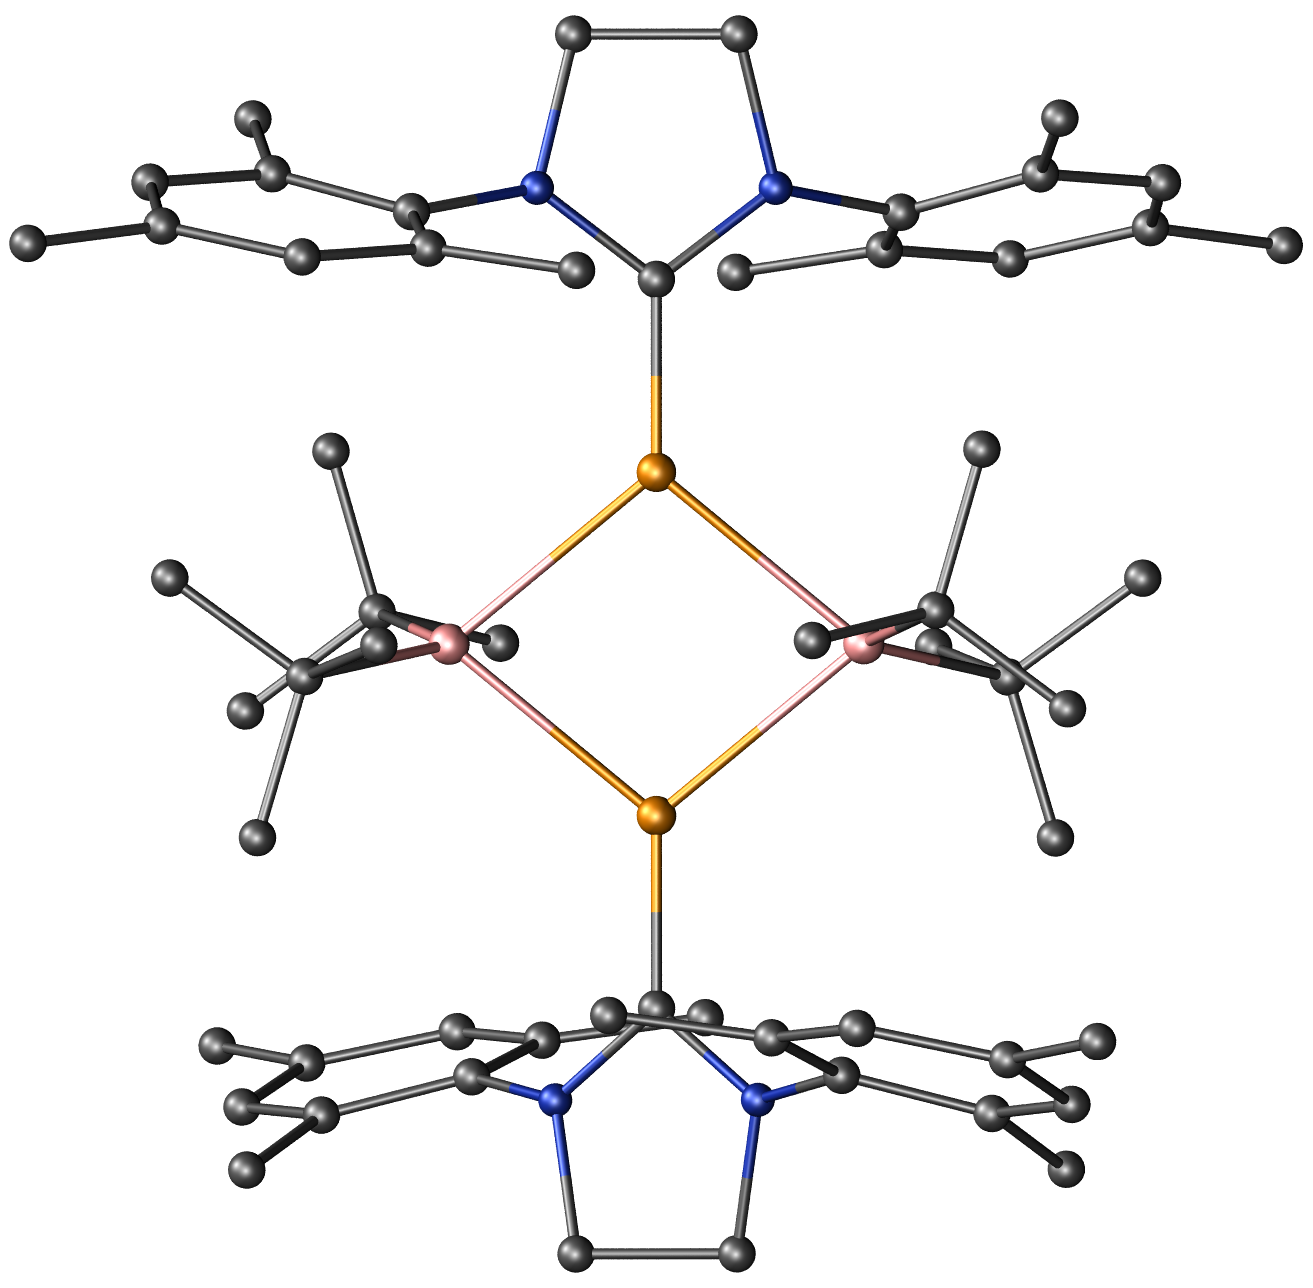
\includegraphics[width=0.6\textwidth]{3}
%	\captionsetup{figurewithin = chapter}
%	\captionsetup{font=small, labelfont=bf}\caption[{Abbildung von $[$SIMesPGa$^\textit{t}$Bu$_2]_2$}]{Abbildung von $[$SIMesPGa$^\textit{t}$Bu$_2]_2$, SIMes=1,3-bis(2,4,6-tri\-me\-thyl\-phe\-nyl)imi\-da\-zo\-lin-2-yli\-den (Kohlenstoff=grau, Stickstoff=blau, Phosphor=orange und Gallium=rosa). Die Wasserstoffatome wurden zur besseren Veranschaulichung bei der Abbildung weg gelassen.}
%\label{abb:cvh3}
%\end{figure}

%\begin{figure}[ht!]
%	\centering
%	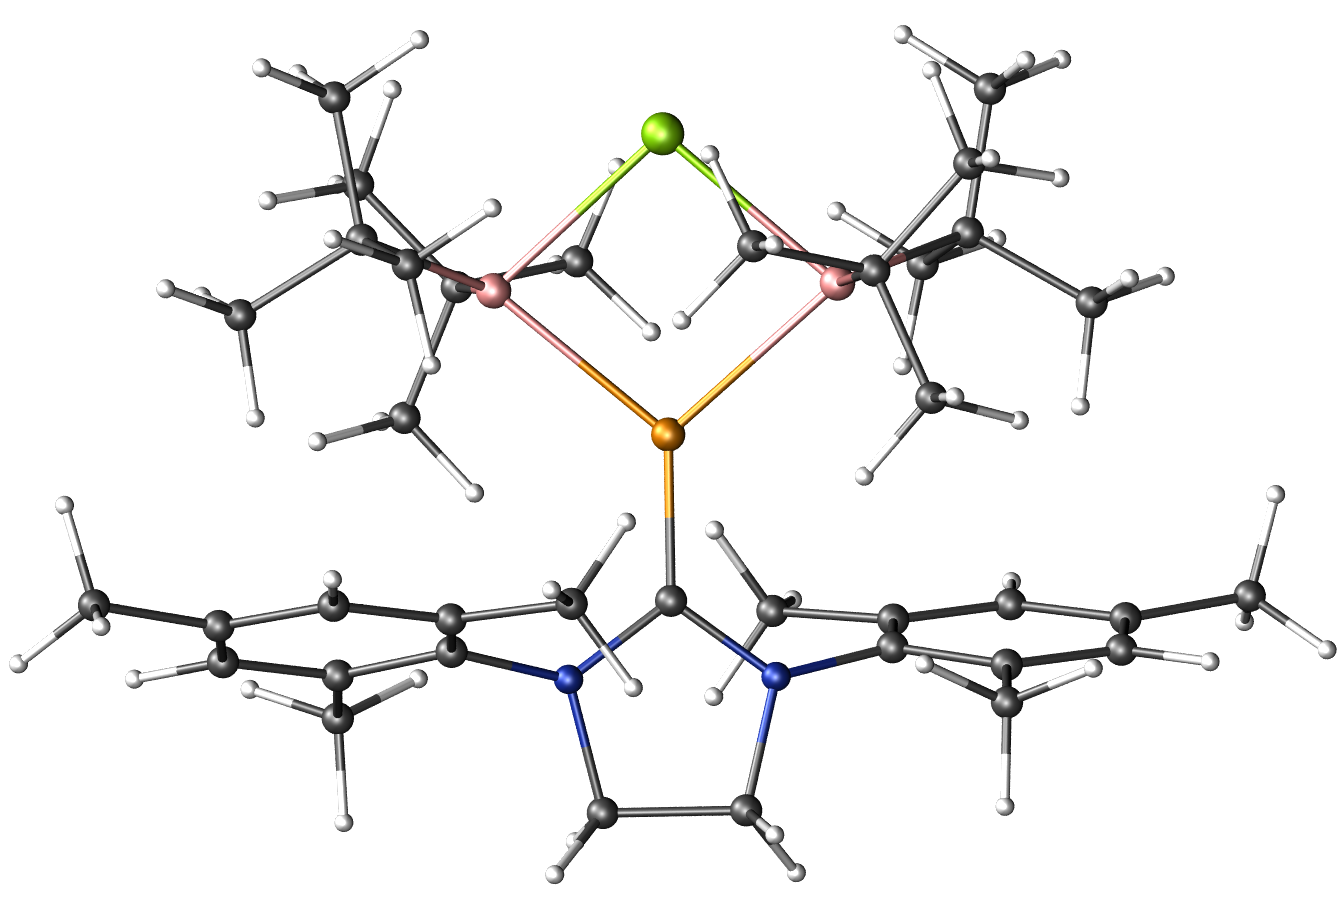
\includegraphics[width=0.6\textwidth]{4}
%	\captionsetup{figurewithin = chapter}
%	\captionsetup{font=small, labelfont=bf}\caption[Abbildung von SIMesP(Ga$^\textit{t}$Bu$_2$)$_2$Cl]{Abbildung von SIMesP(Ga$^\textit{t}$Bu$_2$)$_2$Cl, SIMes=1,3-bis(2,4,6-tri\-me\-thyl\-phe\-nyl)imi\-da\-zo\-lin-2-yli\-den (Kohlenstoff=grau, Wasserstoff=weiß, Stickstoff=blau, Phosphor=orange, Gallium=rosa und Chlor=grün).}
%\label{abb:cvh4}
%\end{figure}
%
%\begin{figure}[ht!]
%	\centering
%	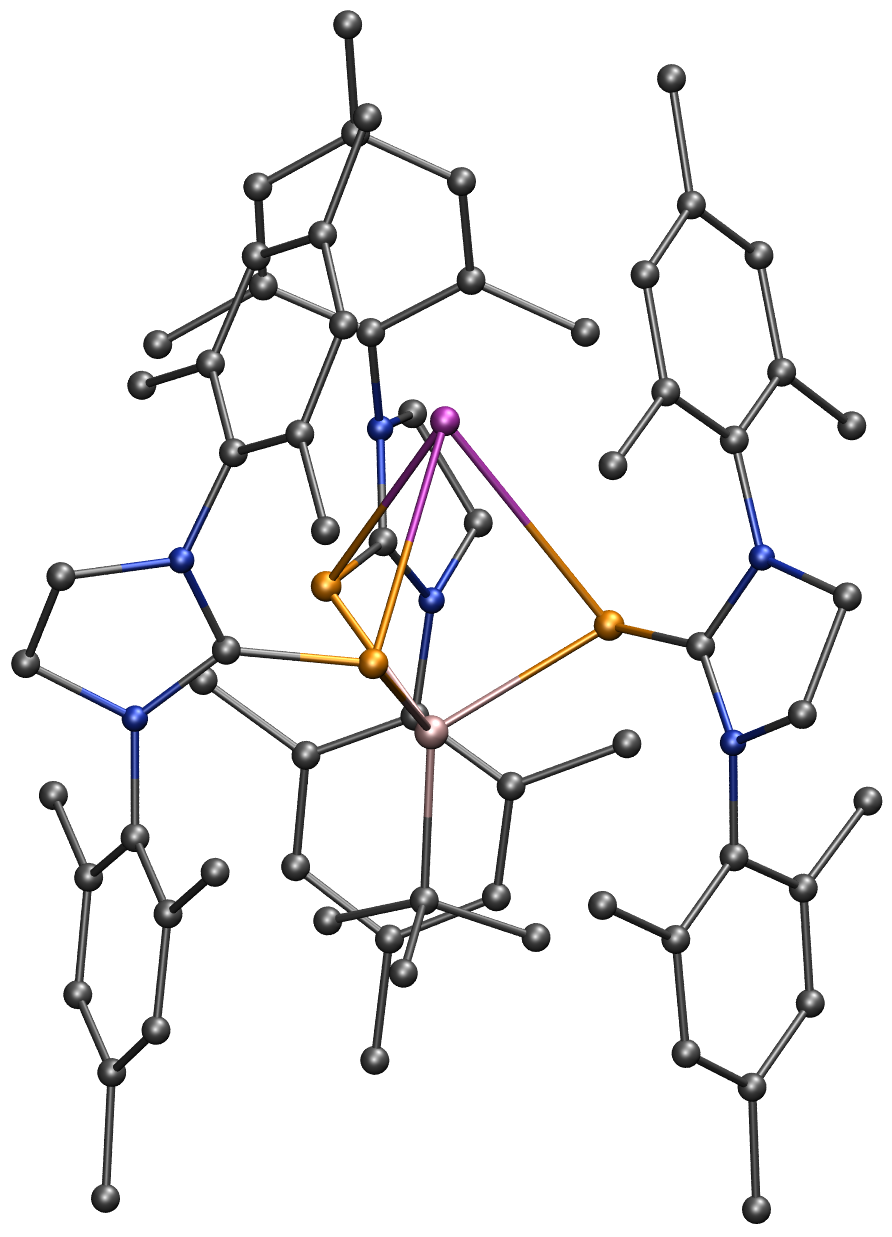
\includegraphics[width=0.5\textwidth]{5}
%	\captionsetup{figurewithin = chapter}
%	\captionsetup{font=small, labelfont=bf}\caption[Abbildung von K(SIMesP)$_3$Al$^\textit{t}$Bu]{Abbildung von K(SIMesP)$_3$Al$^\textit{t}$Bu, SIMes=1,3-bis(2,4,6-tri\-me\-thyl\-phe\-nyl)imi\-da\-zo\-lin-2-yli\-den (Kohlenstoff=grau, Stickstoff=blau, Phosphor=orange, Kalium=lila und Aluminium=hellrosa). Die Wasserstoffatome wurden zur besseren Veranschaulichung bei der Abbildung weg gelassen.}
%\label{abb:cvh5}
%\end{figure}

%\begin{figure}[ht!]
%	\centering
%	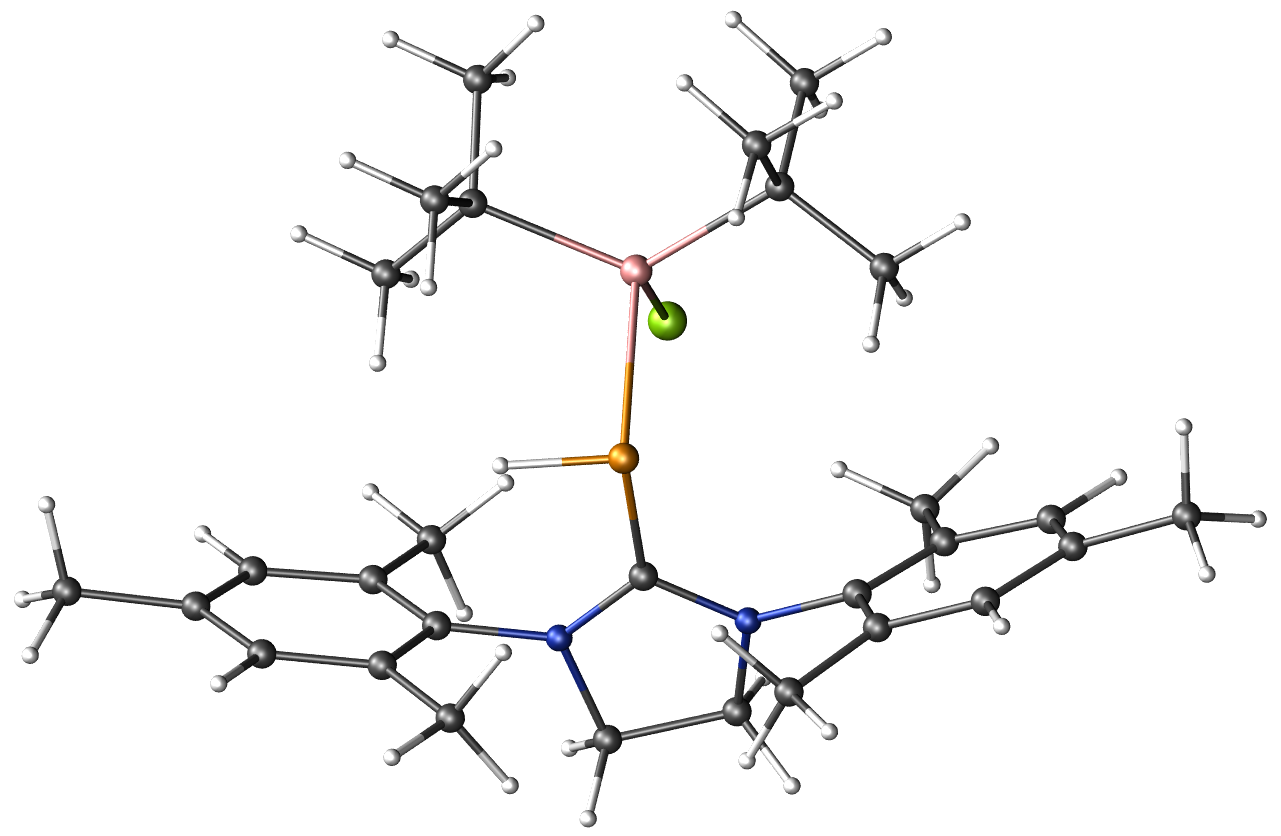
\includegraphics[width=0.6\textwidth]{6}
%	\captionsetup{figurewithin = chapter}
%	\captionsetup{font=small, labelfont=bf}\caption[Abbildung von SIMesPH$^\textit{t}$Bu$_2$GaCl]{Abbildung von SIMesPH$^\textit{t}$Bu$_2$GaCl, SIMes=1,3-bis(2,4,6-tri\-me\-thyl\-phe\-nyl)imi\-da\-zo\-lin-2-yli\-den (Kohlenstoff=grau, Wasserstoff=weiß, Stickstoff=blau, Phosphor=orange, Gallium=rosa und Chlor=grün).}
%\label{abb:cvh6}
%\end{figure}
%
%\begin{figure}[ht!]
%	\centering
%	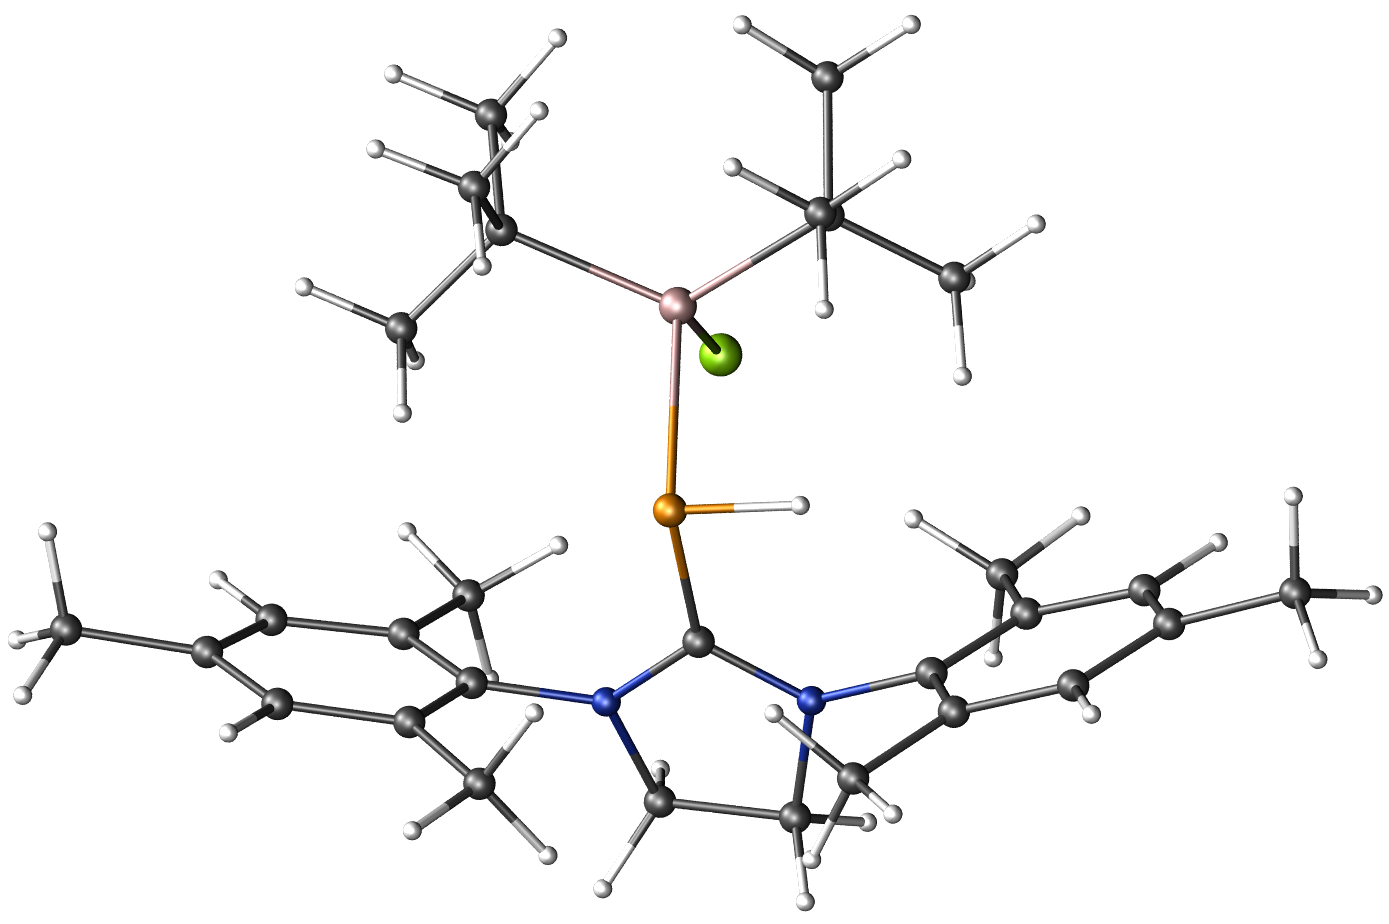
\includegraphics[width=0.6\textwidth]{7}
%	\captionsetup{figurewithin = chapter}
%	\captionsetup{font=small, labelfont=bf}\caption[Abbildung von SIMesPH$^\textit{t}$Bu$_2$AlCl]{Abbildung von SIMesPH$^\textit{t}$Bu$_2$AlCl, SIMes=1,3-bis(2,4,6-tri\-me\-thyl\-phe\-nyl)imi\-da\-zo\-lin-2-yli\-den (Kohlenstoff=grau, Wasserstoff=weiß, Stickstoff=blau, Phosphor=orange, Aluminium=hellrosa und Chlor=grün).}
%\label{abb:cvh7}
%\end{figure}

%\begin{figure}[ht!]
%	\centering
%	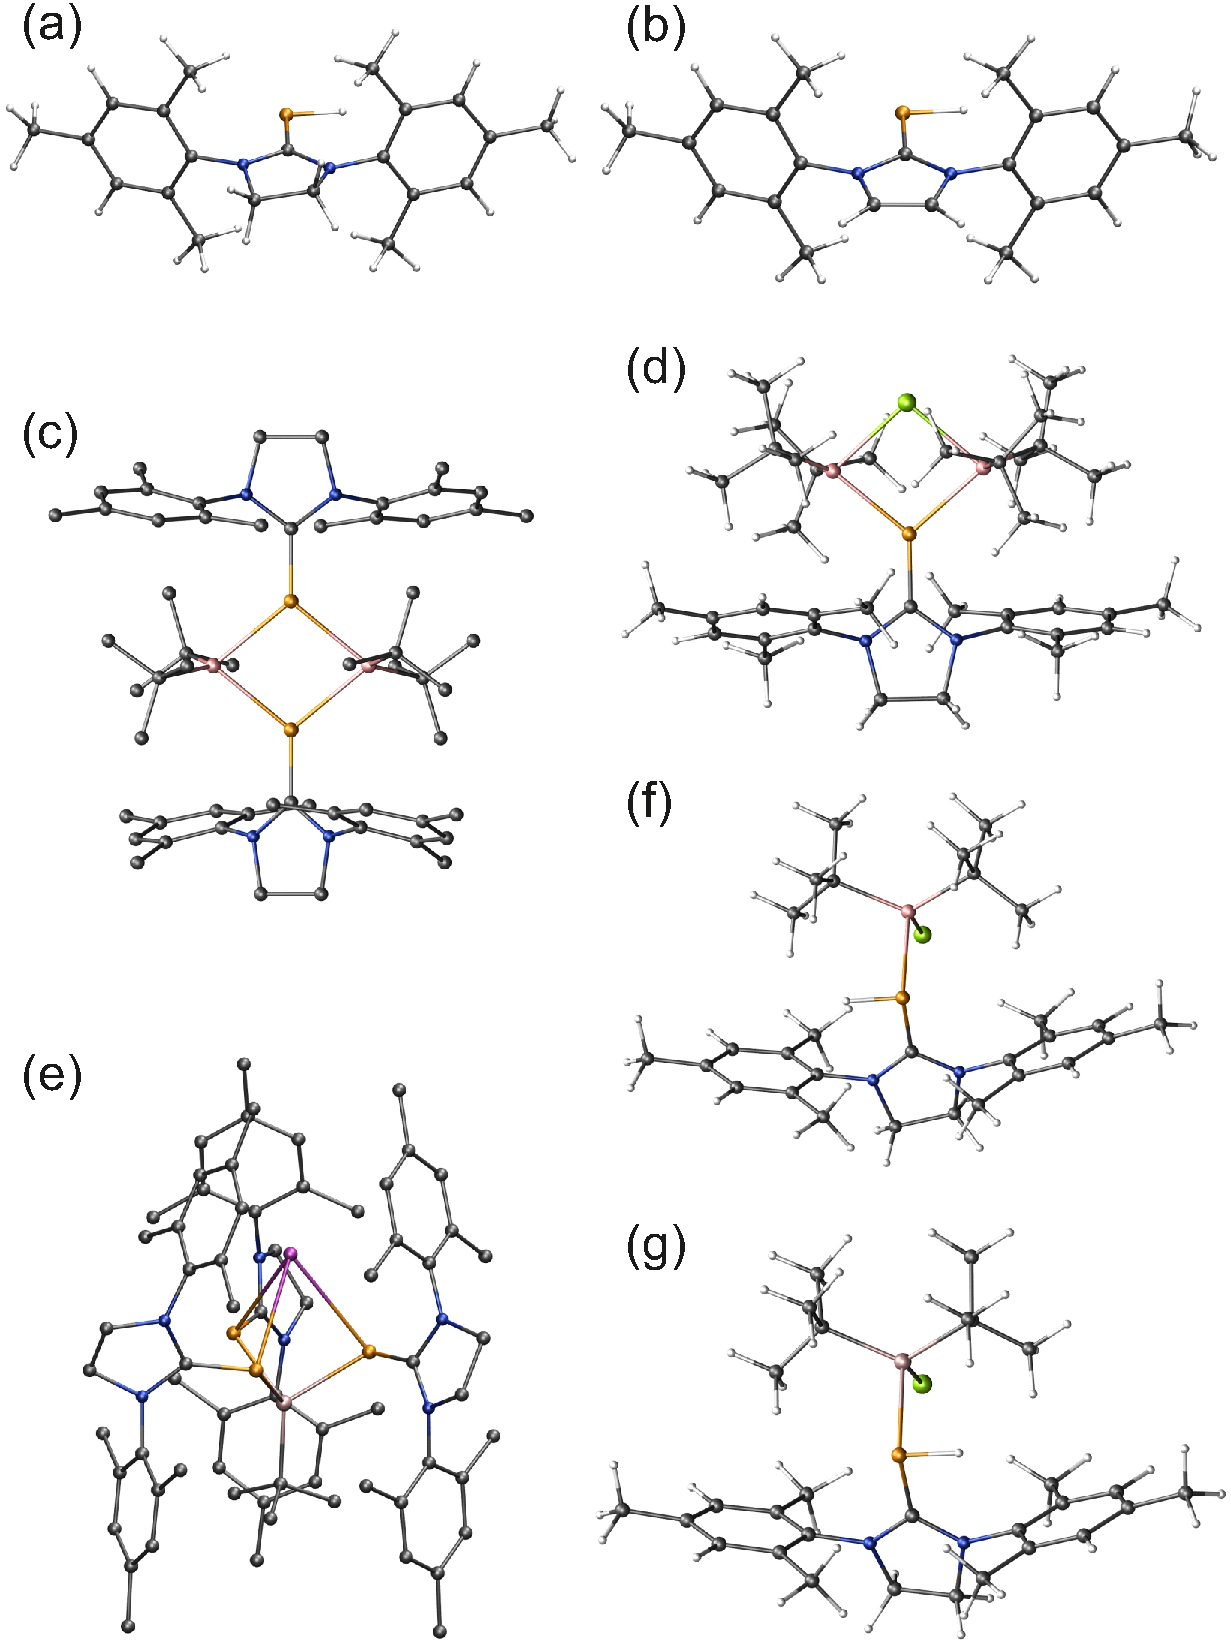
\includegraphics[width=1.0\textwidth]{cvhmols}
%	\captionsetup{figurewithin = chapter}
%	\captionsetup{font=small, labelfont=bf}\caption[Abbildung von SIMesPH$^\textit{t}$Bu$_2$AlCl]{Abbildung von SIMesPH$^\textit{t}$Bu$_2$AlCl, SIMes=1,3-bis(2,4,6-tri\-me\-thyl\-phe\-nyl)imi\-da\-zo\-lin-2-yli\-den (Kohlenstoff=grau, Wasserstoff=weiß, Stickstoff=blau, Phosphor=orange, Aluminium=hellrosa und Chlor=grün).}
%\label{abb:cvh8}
%\end{figure}